\documentclass[a4paper]{book}
\usepackage{mathematics}
\hypersetup{
	pdftitle={Geometria 1},
	pdfauthor={Davide Ferracin},
	pdflang={it},
	pdfsubject={Appunti del corso di Geometria 1},
	pdfcreator={Davide Ferracin},
	pdfcaptionwriter={Davide Ferracin}
	pdfcopyright={Creative Commons Attribution-ShareAlike 4.0 International},
	pdflicenseurl={http://creativecommons.org/licenses/by-sa/4.0/},
	pdfmetalang={it}
}

\title{
	{\sffamily\fontsize{35}{42}\selectfont Geometria 1}
}
\author{
	{\small a cura di}\\
	Davide Ferracin
}
\date{}

\pagestyle{headings}

\begin{document}
\frontmatter

% Frontespizio
\maketitle

% Colophon (informazioni sulla licenza)
\null % Bisogna scrivere qualcosa prima di \vfill, altrimenti non funziona
\vfill % Riempie lo spazio verticale della pagina
\hspace*{-1.5em}
\includegraphics[scale=.7]{by-sa-icon.pdf}
\begin{flushleft}
	Quest'opera è stata rilasciata con licenza \emph{Creative Commons} Attribuzione - Condividi allo stesso modo 4.0 Internazionale. Per leggere una copia della licenza visita il sito web \url{http://creativecommons.org/licenses/by-sa/4.0/}.\\
	2015, Davide Ferracin (\href{mailto:davide.ferracin@studenti.unimi.it}{\ttfamily davide.ferracin@studenti.unimi.it})\\[1cm]
	Versione aggiornata al \today.
\end{flushleft}

\mainmatter

\chapter{Gruppi e anelli}
\section{Gruppi} \label{sec:gruppi}
\begin{definizione} \label{d:gruppo}
Si definisce \emph{gruppo} un insieme $G$ non vuoto munito di un'operazione binaria interna $*\colon G\times G\to G$, ossia tale per cui sono rispettati gli assiomi seguenti:
\begin{enumerate}
\item vale la proprietà associativa, cioè $\forall g_1,g_2,g_3\in G$ vale $g_1*(g_2*g_3)=(g_1*g_2)*g_3$;
\item esiste l'elemento neutro, cioè $\exists e\in G\colon\forall g\in G$, $g*e=e*g=g$;
\item esiste l'inverso, ossia $\forall g\in G$ $\exists g'\in G\colon g*g'=g'*g=e$.
\end{enumerate}
\end{definizione}
Dove non ci saranno ambiguità, d'ora in poi indicheremo l'operazione interna del gruppo come una moltiplicazione, omettendo il simbolo $*$: scriveremo dunque $x*y=xy$. L'inverso di un elemento $x$ sarà indicato, coerentemente, con $x^{-1}$.

La struttura di gruppo si compone sempre di un insieme e di un'operazione, perciò si identifica convenzionalmente con la coppia $(G,*)$; uno insieme può formare gruppi differenti in base all'operazione associata.
Il gruppo è detto \emph{commutativo} (o \emph{abeliano}) se vale anche la proprietà commutativa, cioè $\forall x,y\in G$, $xy=yx$.

L'elemento neutro di un gruppo è sempre unico: se $e$ ed $e'$ rispettano la seconda proprietà, allora $e'=ee'=e$ quindi coincidono.
Lo stesso vale per l'inverso, dato $x\in G$: se $a$ e $b$ sono due inversi di $x$, allora
\begin{equation}
	b=eb=(ax)b=a(xb)=ae=a.
	\label{eq:unicita-inverso}
\end{equation}

Elenchiamo di seguito alcuni esempi, più o meno immediati, di gruppi.
\begin{itemize}
	\item Gli insiemi $\Z$, $\Q$, $\R$, $\C$ con l'usuale operazione di addizione. Più in generale, gli elementi di un campo qualsiasi formano un gruppo rispetto all'addizione.
	\item Gli insiemi $\Q$, $\R$, e $\C$, privati dello zero, con l'usuale moltiplicazione. Lo stesso accade per gli elementi non nulli di un campo qualsiasi: dato un campo $K$, saremo soliti indicare il gruppo moltiplicativo $(K\setminus\{0\},\cdot)$ con il simbolo $K^\times$.
	\item Le rotazioni in un piano, con l'operazione di composizione, che è anche abeliano.
	\item Le rotazioni in $\R^3$, sempre con la composizione, sono ancora un gruppo. Esso però non è abeliano, perch\'e due rotazioni effettuate rispetto ad assi differenti in generale non commutano.
	\item L'insieme $\{-1,1\}$ forma un gruppo rispetto alla moltiplicazione.
\end{itemize}

\begin{definizione} \label{d:sottogruppo}
	Un sottoinsieme $H$ di un gruppo $G$ è detto \emph{sottogruppo} di $G$ se è a sua volta un gruppo con l'operazione di $G$.
\end{definizione}
In altre parole, $H$ è un gruppo contenuto in un gruppo più grande.
Questa definizione equivale alle richieste:
\begin{enumerate}
	\item $H$ deve essere chiuso rispetto all'operazione del gruppo $G$, ossia se $a,b\in H$ allora $ab,ba\in H$;
	\item ogni elemento di $H$ deve avere il suo inverso in $H$.
\end{enumerate}
Di conseguenza, $H$ deve anche contenere l'elemento neutro (lo stesso!) di $G$, poich\'e se $x\in H$, allora anche $x^{-1}$ vi appartiene, dunque anche $xx^{-1}=e$.

Ogni gruppo ammette sempre due sottogruppi: il gruppo stesso e il \emph{sottogruppo banale} $\{e\}$ del suo elemento neutro.
Gli altri sottogruppi, se esistono, sono detti \emph{propri}.
Se un gruppo è abeliano, allora anche tutti i suoi sottogruppi lo sono.
Alcuni esempi di sottogruppi sono i seguenti.
\begin{itemize}
	\item L'insieme $\T=\{z\in\C\colon \abs{z}=1\}$, detto \emph{gruppo circolare}, è un sottogruppo di $\C^\times$.
		Poich\'e $\C^\times$ è abeliano, lo è anche $\T$.
	\item In $\R^2$, sia $R(\theta)$ la rotazione antioraria di un angolo $\theta$.
		L'insieme $\{R(0), R(\pi/2), R(\pi), R(3\pi/2)\}$ è un sottogruppo del gruppo delle rotazioni nel piano.
\end{itemize}

\section{Relazioni di equivalenza} \label{sec:relazioni-equivalenza}
Una relazione binaria su un insieme $X$ lega due elementi dell'insieme.
Essa si definisce come un sottoinsieme di $X\times X$, intendendo che due elementi $a,b$ sono messi in relazione da $R$ se $(a,b)\in R$.
Solitamente una relazione di questo tipo si indica con il simbolo $\sim$, cioè $a\sim b$.
\begin{definizione} \label{d:relazione-equivalenza}
	La relazione $\sim$ è una relazione di equivalenza su $X$ se è binaria e valgono le seguenti proprietà:
	\begin{enumerate}
		\item è riflessiva: $a\sim a$;
		\item è simmetrica: se $a\sim b$, allora $b\sim a$;
		\item è transitiva: se $a\sim b$ e $b\sim c$, allora anche $a\sim c$.
	\end{enumerate}
\end{definizione}
Con questa relazione di equivalenza possiamo ``raggruppare'' gli elementi di $X$ in vari insiemi di elementi tutti in relazione tra loro.
Vediamo se questa suddivisione è buona, cioè se un elemento è categorizzato in uno solo di questi insiemi o meno.
\begin{definizione}
	Si chiama \emph{classe di equivalenza} di un elemento $a\in X$, rispetto alla relazione $\sim$, l'insieme
	\begin{equation*}
		[a]=\{b\in X\colon b\sim a\}.
	\end{equation*}
	L'elemento $a$ è detto \emph{rappresentante} della classe $[a]$.
\end{definizione}
\begin{teorema}
	Due classi di equivalenza, rispetto alla relazione $\sim$, $[a]$ e $[a']$ coincidono se e solo se $a\sim a'$.
\end{teorema}
\begin{proof}
	Siano le due classi $[a]=\{x\in X\colon x\sim a\}$ e $[a']=\{y\in X\colon y\sim a'\}$.
	Sia $[a]\subseteq[a']$: preso un elemento $x\in[a]$, si ha ovviamente che $x\sim a$.
	Poiché $a\sim a'$, per la proprietà transitiva $x\sim a'$ quindi $x\in[a']$, e viceversa per simmetria: allora $[a]\equiv[a']$.
	Poniamo ora le due classi coincidenti, siccome $a\in[a]$ e $a'\in[a']$, poichè le due classi coincidono si ha che $a$ appartiene anche ad $[a']$ e $a'$ appartiene anche ad $[a]$, quindi $a\sim a'$.
\end{proof}

\begin{teorema}
	Due classi di equivalenza sono distinte se e solo se sono disgiunte: se $[a]\neq[b]$ allora $[a]\cap[b]=\emptyset$.
\end{teorema}
\begin{proof}
	Sia per assurdo che esista un elemento $c\in[a]\cap[b]$.
	Allora esso è in relazione sia con $a$ che con $b$, ma allora per la proprietà transitiva $a\sim b$, quindi le due classi coincidono, il che è una contraddizione.
	Le due classi devono quindi essere disgiunte.
\end{proof}

Le classi distinte individuate da una relazione di equivalenza in $X$ costituiscono una partizione di $X$.
\begin{definizione} \label{d:partizione}
	Sia $\{S_i\}_{i\in I}$ una famiglia di sottoinsiemi di un insieme $X$. Tale famiglia si dice \emph{partizione} di $X$ se:
	\begin{itemize}
		\item $S_i\neq\emptyset$ $\forall i\in I$;
		\item $S_i\cap S_j=\emptyset$ per ogni $i\neq j$;
		\item $\bigcup_{i\in I}S_i\equiv X$.
	\end{itemize}
\end{definizione}
Sia $\{S_i\}_{i\in I}$ una partizione di un insieme $X$: si può sempre definire una relazione di equivalenza $\sim$ su $X$, ponendo che $\forall a,b\in X$, $a\sim b$ se e solo se $\exists i\in I\colon a,b\in S_i$.
Una tale relazione soddisfa la definizione di relazione di equivalenza:
\begin{enumerate}
	\item Qualsiasi $a\in X$ sta in almeno uno dei sottoinsiemi $S_i$, per il terzo punto della \ref{d:partizione}, quindi $a\sim a$.
	\item Se esiste un $i\in I$ per cui $a,b\in S_i$, certamente scambiando l'ordine di $b$ e $a$ entrambi appartengono comunque a $S_i$, quindi se $a\sim b$ anche $b\sim a$.
	\item Se $a\sim b$ e $b\sim c$, allora esiste $i\in I$ per il quale $a,b\in S_i$ ed esiste un altro indice $j\in I$ per cui $b,c\in S_j$.
		Se $i\neq j$, però, $b$ non potrebbe appartenere ad entrambi perché la loro intersezione sarebbe vuota.
		Allora $i=j$, e per tale indice $a,b,c\in S_i$ (o $S_j$), quindi $a\sim c$.
\end{enumerate}



\section{Anelli} \label{sec:anelli}
\begin{definizione} \label{d:anello}
Un insieme non vuoto $A$, dotato di due operazioni binarie interne $*$ e $\diamond$, si dice anello se valgono le seguenti proprietà:
\begin{enumerate}
\item $(A,*)$ è un gruppo abeliano;
\item $(A,\diamond)$ è un semigruppo, cioè è solo associativo;
\item $\forall a,b,c\in A$ valgono $(a* b)\diamond c=(a\diamond c)*(b\diamond c)$ e $a\diamond(b* c)=(a\diamond b)*(a\diamond c)$.
\end{enumerate}
\end{definizione}
Intenderemo sempre che la seconda operazione avrà sempre la precedenza sulla prima, se non diversamente specificato: vale a dire, $x* y\diamond z$ significherà $x*(y\diamond z)$; in caso contrario si usano le parentesi dove necessario.
D'ora in poi, per mantenere una notazione più familiare e semplice, ci riferiremo all'operazione $*$ come ad un'\emph{addizione} (e la indicheremo con $+$), e all'operazione $\diamond$ come ad una \emph{moltiplicazione}.
Infatti l'addizione e la moltiplicazione che tutti conosciamo soddisfano questi assiomi, che comunque possono essere generalizzati ad operazioni differenti, come il prodotto tra polinomi o matrici.

L'anello si dice \emph{commutativo} se anche $(A,\cdot)$ è commutativo, cioè $ab=ba$ $\forall a,b\in A$; la commutatività dell'addizione è sempre garantita dal fatto che $(A,+)$ è abeliano.
L'elemento neutro dell'addizione in un anello esiste sempre, dato che $(A,+)$ è un gruppo: indicheremo tale elemento con $0$, o con $0_A$ se ci sarà bisogno di specificare l'anello al quale appartiene.
L'esistenza dell'elemento neutro della moltiplicazione, invece, non è data per certa: se esiste, l'anello si dice \emph{dotato di unità}, e la indicheremo con $1$ o $1_A$.

Ecco alcuni esempi di anelli.
\begin{itemize}
\item $\Z$ è un anello con le usuali operazioni di addizione e moltiplicazione, come del resto $\Q$, $\R$, $\C$ e ogni altro campo.
%\item Fissato un numero $n$ intero e non nullo, si stabilisce la relazione $\sim$ definita come $a\sim b\iff n\divides a-b$, ossia $n$ divide la differenza $a-b$. Si scrive anche che $a\equiv b\mod n$.
%Si dimostra che $\sim$ così definita è una relazione di equivalenza e congruenza.
%L'insieme delle classi di equivalenza distinte, indicato con $\Z_n$, è un anello rispetto alle operazioni di somma e prodotto definite come segue: $\forall [a]_n,[b]_n\in\Z_n$, $[a]_n+[b]_n=[a+b]_n$ e $[a]_n[b]_n=[ab]_n$. La classe $[1]_n$ è l'unità (per qualsiasi $n$) per il prodotto; inoltre, $[a]_n\equiv[b]_n$ se e solo se $a\sim b$ cioè $b=a+kn$, quindi $[a]_n=\{a+kn,\ k\in\Z\}$.
\item L'insieme $K[x]$ dei polinomi (di grado qualunque) con termini presi da un campo $K$ forma un anello con le note operazioni di somma e prodotto tra polinomi.
\end{itemize}

Definiamo per $n\in\Z$ l'addizione di $a$ con se stesso $n-1$ volte come
\begin{equation}
	na=\underbracket[.5pt]{a+a+\cdots+a}_\textup{$n$ volte},
\end{equation}
per $n\in\N$, e con $0a=0_A$; per $n<0$, basta porre $na=-(-n)a$ per ricondursi ai casi precedenti.
Definiamo poi $a$ moltiplicato con se stesso $n-1$ volte come
\begin{equation}
	a^n=\underbracket[.5pt]{a\cdot a\cdot a\cdots a}_\textup{$n$ volte}
\end{equation}
con $n>0$, e (se esiste l'unità) $a^0=1_A$.
Per $n<0$ questa operazione non è definita.

Ricaviamo alcune semplici proprietà delle due operazioni.
\begin{itemize}
	\item $0_Aa=a0_A=0_A$.
		Possiamo infatti scrivere sempre $0_Aa=(0_A+0_A)a$, e per la proprietà distributiva abbiamo $0_Aa=0_Aa+0_Aa$, per cui aggiungendo l'opposto $-0_Aa$ ai due membri (esiste sempre, essendo $(A,+)$ un gruppo) troviamo $0_aa=0$.
		La dimostrazione è analoga per $a0_A$.
	\item $(na)b=a(nb)=n(ab)$, che di dimostra facilmente sfruttando la proprietà distributiva partendo da $(a+a+\dots+a)b$.
	\item $a(-b)=(-a)b=-(ab)$, ponendo $n=-1$ nella precedente.
\end{itemize}

\begin{definizione} \label{d:divisore-zero}
Un elemento $a\neq 0_A$ di un anello $A$ si dice \emph{divisore dello zero} se esiste un elemento $b\in A$ tale che $ab=0_A$ oppure $ba=0_A$.
\end{definizione}
Ovviamente i due casi coincidono se l'anello è commutativo, ma in generale non lo si può affermare.
\paragraph{Esempi}
\begin{itemize}
	\item L'insieme $\cont{}(-1,1)$ delle funzioni $f\colon(-1,1)\to\R$ continue è un anello con addizione e moltiplicazione.
			In esso, definiamo le funzioni
			\begin{equation*}
				f(x)=
				\begin{cases}
					0& -1<x<0\\
					x^2&0\le x<1
				\end{cases}\qquad\text{e}\qquad
				g(x)=
				\begin{cases}
					x^2& -1<x<0\\
					0&0\le x<1
				\end{cases}
			\end{equation*}
			La $f$ è un divisore dello zero, in quanto $g$ non è la funzione identicamente nulla di $\cont{}(-1,1)$, ma $fg=0$ per ogni $x\in(-1,1)$.
			Per lo stesso motivo, ovviamente, anche $g$ è divisore dello zero.
\begin{comment}
		\item Nell'anello $\mat_{2,2}(\R)$, la matrice $\begin{psmallmatrix}1&0\\0&0\end{psmallmatrix}$ è un divisore dello zero perché
		\begin{equation*}
			\begin{pmatrix}1&0\\0&0\end{pmatrix}\begin{pmatrix}0&0\\1&0\end{pmatrix}=\begin{pmatrix}0&0\\0&0\end{pmatrix}.
		\end{equation*}
	Tale proprietà può essere estesa alle matrici $2\times 2$ in un campo $K$ generico, utilizzando l'unità e lo zero $1_K$ e $0_K$.
		\item In $\Z_{10}$, si prendano le classi $[2]_{10}$ e $[5]_{10}$. Entrambe non sono nulle, perché 2 e 5 non sono divisibili per 10 (non valgono le relazioni $2\equiv 0\mod 10$ e $5\equiv 0\mod 10$). Moltiplicandole, però, risulta $[2]_{10}[5]_{10}=[10]_{10}=[0]_{10}$, perché ovviamente 10 è divisibile per se stesso, quindi $[2]_{10}$ è un divisore dello zero in $\Z_{10}$. Per la commutatività dell'anello, anche $[5]_{10}$ lo è.
	Più in generale, in un anello $\Z_n$ sono divisori dello zero le classi $[a]_n$ dove $a$ è un divisore non banale di $n$.
\end{comment}
\end{itemize}

\begin{teorema}
	Un anello $A$ è privo di divisori dello zero se e solo se valgono le leggi di cancellazione per il prodotto.\footnote{Ossia se per ogni $a,x,y\in A$ con $a\ne 0$ le relazioni $ax=ay$ e $xa=ya$ implicano $x=y$.}
\end{teorema}
\begin{proof}
	Supponiamo che $A$ sia un anello privo di divisori dello zero, e prendiamo l'ipotesi $ax=ay$: dalla proprietà distributiva si ha $a(x-y)=0$.
	Dato che non esistono divisori dello zero in $A$, se $a\ne 0$ deve necessariamente essere $x-y=0$, ossia $x=y$.
	La dimostrazione per $xa=ya\then x=y$ è del tutto analoga.
	
	Partiamo ora dalle relazioni $ax=ay\then x=y$ e $xa=ya\then x=y$.
	Se esistessero $x,y\ne 0$ tali che $xy=0$ (ossia $x$ e $y$ divisori dello zero), allora risulterebbe anche $xy=0=x0$ da cui $y=0$, poich\'e valgono le leggi di cancellazione del prodotto.
	Ma ciò contraddice l'ipotesi che $x,y\ne 0$ quindi tali $x$ e $y$ non possono esistere: allora $A$ è privo di divisori dello zero.
\end{proof}

\begin{definizione} \label{d:elemento-invertibile}
	Sia $A$ un anello con unità.
	Un elemento $a\in A$ si dice \emph{invertibile} se esiste $b\in A$ tale per cui $ab=ba=1$.
	Tale $b$ si indica con $a^{-1}$.
\end{definizione}

\begin{teorema}
	Se $A$ è un anello dotato di unità, i suoi elementi invertibili non sono divisori dello zero.
\end{teorema}
\begin{proof}
	Se esistesse un elemento $a\in A$ invertibile e divisore dello zero, allora esisterebbe un elemento $b\in A\setminus\{0\}$ tale che $ab=0$.
	Si ottiene però che
	\begin{equation}
		b = 1b = a^{-1}ab = a^{-1}0 = 0
	\end{equation}
	ossia $b=0$, che contraddice l'ipotesi $b\ne 0$ legata all'esistenza di $b$.
	Dunque non può esistere un tale $b$: vale a dire, $a$ non è un divisore dello zero.
\end{proof}

\begin{definizione} \label{d:dominio-integrita}
	Un anello si dice \emph{dominio d'integrità} se è commutativo ed è privo di divisori dello zero.
\end{definizione}
Sono domini d'integrità gli anelli di $\Z$, $\Q$, $\R$, $\C$ con le usuali operazioni di somma e prodotto.

\begin{definizione}
Si chiama \emph{corpo} un anello dotato di unità in cui ogni elemento non nullo è invertibile.
\end{definizione}

\begin{definizione} \label{d:campo1}
Si dice \emph{campo} un corpo commutativo con almeno due elementi.
\end{definizione}
Il piccolo teorema di Wedderburn afferma, inoltre, che ogni corpo finito è un campo.
Possiamo dare una definizione alternativa di campo, equivalente alla precedente, basata su degli assiomi.
\begin{definizione} \label{d:campo2}
Si definisce \emph{campo} la terna $(K,+,\cdot)$ in cui $K$ è un insieme non vuoto e $+$ e $\cdot$ sono operazioni interne $K\times K\to K$, per le quali:
\begin{itemize}
\item $(K,+)$ è un gruppo abeliano, con elemento neutro $0_K$;
\item $(K\setminus\{0_K\},\cdot)$ è un gruppo abeliano, con elemento neutro $1_K$;
\item vale la proprietà distributiva, per cui $\forall a,b,c\in K$ vale $a\cdot(b+c)=a\cdot b+a\cdot c$.
\end{itemize}
\end{definizione}
Questa definizione è in sostanza una generalizzazione della struttura di $(\R,+,\cdot)$. È quindi, ovviamente, un campo $(\R,+,\cdot)$, e lo sono anche $(\Q,+,\cdot)$ e $(\C,+,\cdot)$.


\section{Ideali} \label{sec:ideali}
\begin{definizione} \label{d:ideale}
	Sia $A$ un anello e $I$ un suo sottoinsieme.
	Se $(I,+)$ è un sottogruppo di $(A,+)$ e per ogni $x\in I$ e $a\in A$:
	\begin{itemize}
		\item $ax\in I$, allora $I$ è detto \emph{ideale sinistro};
		\item $xa\in I$, allora $I$ è detto \emph{ideale destro};
		\item $ax,xa\in I$, allora $I$ è detto \emph{ideale bilatero}.
	\end{itemize}
\end{definizione}
In altre parole, preso un elemento di un ideale sinistro (destro) possiamo moltiplicarlo a sinistra (destra) per qualsiasi elemento dell'anello e ottenere ancora un elemento dell'ideale.
Nel caso di un anello commutativo, le tre definizioni naturalmente coincidono, e parleremo semplicemente di \emph{ideale}.

Dalla chiusura di $I$ rispetto alla somma otteniamo inoltre che qualsiasi ideale deve sempre contenere lo zero dell'anello.
Ogni anello ammette sempre due ideali detti \emph{banali}: $\{0\}$ e l'anello $A$ stesso.
Gli ideali non banali sono detti \emph{propri}.
Se l'anello è dotato di unità, allora un ideale è proprio se e solo se non la contiene: se infatti $I\ni 1$, allora poich\'e il prodotto $1a$ per qualsiasi $a$ nell'intero anello deve essere incluso in $I$, tale ideale contiene tutti gli elementi di $A$, ma allora $I=A$.

Degli esempi importanti di ideali, che incontreremo in seguito, sono i seguenti.
\begin{itemize}
	\item Dato $p\in\Z$, chiamiamo $p\Z$ l'insieme $\{x\in\Z\colon x=np, n\in\Z\}$ ossia l'insieme dei multipli interi di un certo intero $p$.
		Se $x,y\in p\Z$, siano essi $x=np$ e $y=mp$, allora $x+y=(n+m)p$ e poich\'e $n+m\in\Z$ allora $x+y\in p\Z$.
		Per un qualunque $z\in\Z$, inoltre, $xz=npz=(nz)p$ e $nz\in\Z$ quindi $xz\in p\Z$.
		L'insieme $p\Z$ è dunque un ideale di $\Z$, per qualunque $p$.
	\item I numeri pari formano l'insieme $2\Z$, che è un ideale per il punto precedente.
		I numeri dispari, invece, non formano un ideale, in quanto non comprendono lo zero.
	\item Nell'anello delle funzioni continue $\cont{}(\R)$, è un ideale l'insieme delle funzioni che si annullano in un dato punto, ad esempio per cui $f(1)=0$.
\end{itemize}

Definiamo ora alcuni tipi particolari di ideali (per semplicità, le daremo per anelli commutativi).
\begin{definizione} \label{d:ideale-primo}
	Un ideale $I$ di un anello $A$ è detto \emph{primo} se:
	\begin{itemize}
		\item è un sottoinsieme proprio di $A$;
		\item se $a,b\in A$ sono tali che $ab\in I$, allora almeno uno dei due appartiene a $I$.
	\end{itemize}
\end{definizione}
Questo concetto ricalca la definizione di \emph{numeri primi}: se un numero $p\in\Z$ è primo, ogni volta che divide un prodotto $xy$ con $x,y\in\Z$ allora $p$ divide $a$ oppure $b$.
Le due definizioni sono in effetti collegate: un numero intero (positivo) $n$ è primo se e solo se $n\Z$ è un ideale primo.
 
\begin{definizione} \label{d:ideale-massimale}
	Un ideale $A$ si dice \emph{massimale} se $I\neq A$, per ogni ideale $J\supseteq I$ si ha o che $J=I$ oppure $J=A$.
\end{definizione}
Gli ideali massimali sono dunque degli elementi massimali rispetto all'operazione di inclusione insiemistica tra gli \emph{ideali propri} di un anello (escludendo quindi dalle opzioni l'anello stesso).
Essi non sono contenuti propriamente in nessun altro ideale proprio dell'anello.

Se ogni elemento $x$ di un ideale $I$, di un anello $A$, può essere scritto come
\begin{equation*}
	x=\sum_{i=1}^na_ki_k
\end{equation*}
con $a_k\in A$ e $i_k\in I$, ossia come combinazione lineare di un numero finito di suoi elementi $\{i_k\}_{k=1}^n$, diciamo che l'ideale è \emph{generato} da tali elementi, e si indica solitamente come $I=(i_1,\dots,i_n)$.
Il caso in cui l'ideale è generato da un solo elemento è di particolare importanza, e merita una sua definizione.
\begin{definizione} \label{d:ideale-principale}
	Un ideale $I$ di un anello $A$ si dice \emph{principale} se è generato da un solo elemento.
\end{definizione}
In linea con la notazione precedente, l'ideale principale generato da $a$ si indica con $(a)$.
Si può dimostrare che l'ideale principale $(a)$ è il più piccolo ideale che comprende $a$.

\section{Anelli quoziente} \label{sec:anelli-quoziente}
Riprendiamo ora le relazioni di equivalenza, introdotte nel capitolo \ref{sec:relazioni-equivalenza}.
Dati un ideale (bilatero) $I$ di un anello $A$ e due elementi $a,b\in A$, stabiliamo la relazione
\begin{equation*}
	a\sim b\iff a-b\in I.
\end{equation*}
È facile vedere, con le proprietà degli ideali, che tale relazione è anche di congruenza.
Se $a\sim b$ si dice anche che $a$ e $b$ sono \emph{congruenti modulo $I$}.
Da essa possiamo costruire le classi di equivalenza nell'anello: la classe $[a]_I$ (indichiamo con il pedice $[\cdot]_I$ il fatto che la relazione è basata sull'ideale $I$, per maggiore chiarezza) consiste in tutti quegli elementi $x$ di $A$ che ``distano $a$ dall'ideale $I$'', ossia tali per cui $x-a\in I$.
Alternativamente, gli elementi $x\in[a]_I$ sono la somma di $a$ e di un elemento dell'ideale $I$, e per questo motivo si indica la classe di equivalenza come $I+a$.
Formalmente, dunque,
\begin{equation*}
	[a]_I=I+a=\{x\in A\colon x=a+i, i\in I\}.
\end{equation*}
Possiamo definire delle operazioni su queste classi come di seguito:
\begin{itemize}
	\item l'addizione di $[a]_I=I+a$ e $[b]_I=I+b$ come la classe di rappresentante $a+b$, ossia $I+(a+b)$;
	\item analogamente, la moltiplicazione di due classi $[a]_I[b]_I=(I+a)(I+b)$ come la classe che ha come rappresentante il prodotto dei due rappresentanti, ossia $I+ab$.
\end{itemize}
Si può verificare che queste operazioni sono ben definite, ossia che non dipendono dalla scelta dei rappresentanti.
Con queste due operazioni, l'insieme delle classi di equivalenza forma un anello, detto \emph{anello quoziente} (rispetto alla relazione stabilita).

\begin{definizione} \label{d:anello-quoziente}
	Dato un ideale bilatero $I$ di un anello $A$, si chiama \emph{anello quoziente} l'insieme, indicato con $A\quot I$, delle classi di equivalenza $[a]_I=\{x\in A\colon x=a+i, i\in I\}$, con le operazioni
	\begin{equation}
		\begin{gathered}
			(I+a)+(I+b)=I+(a+b)\\ (I+a)(I+b)=I+ab.
		\end{gathered}
		\label{eq:operazioni-anello-quoziente}
	\end{equation}
\end{definizione}
Lo zero dell'anello quoziente è indicato come $I+0$, ed è chiaramente l'ideale $I$ stesso.
Notiamo che se $a\in I$, allora $I+a$ è ancora lo zero di $A\quot I$: infatti, essendo $I$ chiuso rispetto alla somma, l'addizione di un elemento dell'ideale (cioè $I$) con $a$ (che è in $I$) produce ancora un elemento nell'ideale, vale a dire un elemento di $I=I+0$.
L'identità moltiplicativa, se esiste, sarà indicata con $I+1$.

Proviamo a prendere il quoziente di $A$ con gli ideali banali.
\begin{itemize}
	\item Per $I=\{0\}$, scelto un $a\in A$ abbiamo che $b\in [a]=I+a$ se $b-a\in I$, cioè $b-a=0$: ma ciò è possibile solo se $b=a$, dunque $I+a=\{a\}$ per qualsiasi $a\in A$.
	\item Per $I=A$, se $b\in I+a$ dovrà essere $b-a\in A$: questo è sempre vero qualsiasi sia $b$, quindi $I+a=A$ per qualsiasi $a$!
		Ciò significa che $A\quot A$ è composto da un solo elemento.
\end{itemize}

L'ideale $I=2\Z$ di $\Z$ è massimale: infatti se un ideale $J$ contiene $I$, allora $J=k\Z$ per un $k\in N$ che sia divisore di 2.
Ma allora $k\in\{1,2\}$, cioè $k\Z$ è ancora $2\Z$ oppure è tutto $\Z$.
Perciò $2\Z$ è un ideale massimale; lo stesso di dimostra per qualsiasi $p\Z$ con $p$ primo.
Questo risultato si generalizza nel seguente teorema.
\begin{teorema} \label{t:ideale-primo-quoziente-integro}
	Sia $A$ un anello commutativo con unità e sia $I\subset A$ un ideale proprio: allora $I$ è primo se e solo se $A/I$ è un dominio d'integrità.
\end{teorema}
\begin{proof}
	Supponiamo che $A\quot I$ sia un dominio di integrità, per cui prese due classi $I+a$ e $I+b$, se $I+ab=I+0$ deve necessariamente risultare $I+a=I+0$ oppure $I+b=I+0$.
	Passando dalle classi di $A\quot I$ agli elementi di $A$, il fatto che $I+ab$ sia $I+0$ significa che $ab$ è nell'ideale $I$.
	Analogamente se $I+a=I+0$ significa che $a\in I$.
	Ma ciò vuol dire che se $ab\in I$ allora uno dei due tra $a$ e $b$ è necessariamente nell'ideale: questa è proprio la definizione di ideale primo, quindi $I$ è primo.

	Sia ora $I$ un ideale primo: se $ab\in I$, almeno uno tra $a$ e $b$ deve appartenere a $I$.
	Nel linguaggio delle classi di equivalenza ciò significa che se $(I+a)(I+b)=I+ab=I+0$, allora $I+a=I+0$ oppure $I+b=0$.
	Queste affermazioni sono equivalenti a dire che non esistono $a,b\notin I$ tali che $ab\in I$, cioè
	\begin{equation*}
		\nexists I+a, I+b\in A\quot I\colon (I+a)(I+b)=I+0
	\end{equation*}
	quindi $A\quot I$ è un dominio di integrità.
\end{proof}

\begin{teorema} \label{t:ideale-massimale-quoziente-campo}
	Sia $A$ un anello commutativo con unità e sia $I\subset A$ un ideale proprio: $I$ è massimale se e solo se $A/I$ è un campo.
\end{teorema}
\begin{proof}
	Sia $I$ un ideale massimale: allora non può esistere un ideale $J$ tale che $I\subset J\subset A$.
	Dimostriamo che $A\quot I$ è un campo mostrando che ogni suo elemento non nullo è invertibile.
	Sia $I+a$ un elemento non nullo di $A\quot I$, ossia deve essere $a\notin I$.
	Fissato questo elemento, costruiamo l'insieme $J_a=\{j\in A\colon j=i+ax, i\in I, x\in A\}$.
	Sicuramente, poich\'e $A$ è commutativo, lo è anche $J_a$.
	Inoltre è anche un ideale: infatti, dati $j_1=i_1+ax_1$, $j_2=i_2+ax_2$ e $b\in A$ abbiamo
	\begin{equation}
		\begin{gathered}
			j_i+j_2=\underbracket[.5pt]{i_1+i_2}_{\in I}+a(\underbracket[.5pt]{x_1+x_2}_{\in A})\in J_a;\\
			j_1b=(i_1+ax_1)b=\underbracket[.5pt]{i_1b}_{\in I}+a(\underbracket[.5pt]{x_1b}_{\in A})\in J_a.
		\end{gathered}
	\end{equation}
	Tutti gli elementi $i\in I$ sono della forma $i+a0$, dunque $I\subseteq J$.
	Esistono anche elementi di $J$ che non appartengono a $I$?
	Dato che $I$ è proprio, non può contenere l'unità, come avevamo già visto.
	Allora l'elemento $i+a1=i+a$ appartiene a $J$, ma non a $I$.\footnote{Se $i+a\in I$, ossia $i+a=i'$ per qualche $i'\in I$, allora seguirebbe che $a=i'-i$, cioè $a\in I$.}
	Di conseguenza $I\subset J$: per la massimalità di $I$, però, ciò implica $J\equiv A$.
	Perciò $J$ deve contenere l'unità, che potremo dunque scrivere come $i^*+ax^*$ per qualche $i^*\in I$ e $x^*\in A$.
	Preso questo $x^*$, vediamo che la classe $I+x^*\in A\quot I$ è l'inverso di $I+a$:
	\begin{equation}
		(I+x^*)(I+a)=I+ax^*=I+(1-i^*)=I+1
	\end{equation}
	poich\'e se $i^*+ax^*=1$ allora $ax^*=1-i^*$, e $I-i^*= I$.
	Ma $I+1$ è l'unità di $A\quot I$, dunque ogni elemento non nullo (ossia con $a\notin I$) di $A\quot I$ ammette un inverso: ciò prova che $A\quot I$ è un campo.

	Sia ora $A\quot I$ un campo: allora, poich\'e deve possedere almeno due elementi, $I$ non può essere uguale ad $A$, perch\'e come abbiamo già visto $A\quot A$ contiene un solo elemento.
	Dunque $I$ è un ideale proprio.
	Prendiamo ora un ideale $J$ tale che $I\subseteq J\subseteq A$ con $I\ne J$.
	Esiste dunque un $x$ che appartiene a $J$ ma non a $I$, di conseguenza $I+x\ne I+0$.
	Non essendo l'elemento nullo di $A\quot I$, che per ipotesi è un campo, $I+x$ è invertibile: esiste una classe $I+y\in A\quot I$ tale per cui
	\begin{equation*}
		I+1=(I+y)(I+x)=I+xy,
	\end{equation*}
	quindi $xy=1+i^*$ per qualche $i^*\in I$.
	Ora, $I\subseteq J$, perciò $i^*\in J$, e analogamente $x\in J$ quindi anche $xy\in J$: ma allora anche $1=xy-i^*$ appartiene a $J$.
	Dato che $J$ contiene l'unità, segue necessariamente che $J=A$, perciò $I$ è massimale.
\end{proof}
\begin{corollario} \label{c:ideale-massimale-primo}
	In un anello commutativo con unità, ogni ideale massimale è primo.
\end{corollario}
\begin{proof}
	Se $I$ è massimale, per il teorema \ref{t:ideale-massimale-quoziente-campo} $A\quot I$ è un campo, quindi in particolare è anche un dominio di integrità: ma allora dal teorema \ref{t:ideale-primo-quoziente-integro} $I$ è primo.
\end{proof}
L'implicazione inversa, ossia che ogni ideale primo è massimale, in generale è falsa (il problema sta nell'affermazione ``un campo è un dominio d'integrità'', che non si può invertire).
Vedremo in che ambito essa è vera quando introdurremo i domini \emph{a ideali principali}.

\section{Omomorfismi di anelli}
\begin{definizione} \label{d:omomorfismo-anelli}
	Siano $(A,+,\cdot)$ e $(B,*,\diamond)$ due anelli: un \emph{omomorfismo} di anelli è un'applicazione $\phi\colon A\to B$ che preserva le operazioni, cioè tale che per ogni $a,b\in A$ si ha 
	\begin{equation}
		\phi(a+b)=\phi(a)*\phi(b)\text{ e }\phi(ab)=\phi(a)\diamond\phi(b).
	\end{equation}
	Se gli anelli sono dotati di unità, si richiede che l'omomorfismo, oltre alle operazioni, preservi anche l'unità, ossia $\phi(1_A)=1_B$.
\end{definizione}
Ad esempio la funzione da $\Z$ in s\'e definita come $\phi(a)=0$ per qualsiasi $a\in\Z$, cioè che porta qualsiasi elemento nello zero, chiaramente preserva le operazioni, ma non è un omomorfismo d'anelli in quanto $\phi(1)=0$ che ovviamente non è l'unità di $\Z$.

\begin{definizione} \label{d:nucleo-omomorfismo-anelli}
	Sia $\psi\colon A\to B$ un omomorfismo di anelli. Si definisce \emph{nucleo} di $\psi$ e si denota con $\Ker\psi$ l'insieme
	\begin{equation*}
		\Ker\psi=\{a\in A\colon\psi(a)=0_B\},
	\end{equation*}
	ossia l'insieme degli elementi di $A$ che hanno lo zero di $B$ come immagine.
\end{definizione}

\begin{teorema} \label{t:nucleo-ideale}
	Se $\psi\colon A\to B$ è un omomorfismo di anelli, allora il suo nucleo è un ideale di $A$.
\end{teorema}
\begin{proof}
	Verifichiamo le proprietà di ideale: per $x,y\in\Ker\psi$ e $a\in A$, si ha
	\begin{equation}
		\psi(x+y)=\psi(x)+\psi(y)=0_B+0_B=0_B
	\end{equation}
	quindi $x+y\in\Ker\psi$, e
	\begin{equation}
		\psi(ax)=\psi(a)\psi(x)=\psi(a)0_B=0_B
	\end{equation}
	quindi anche $ax\in\Ker\psi$, e analogamente per $xa$.
	Allora $\Ker\psi$ è proprio un ideale di $A$.
\end{proof}
Come già visto negli omomorfismi tra gruppi, anche un omomorfismo tra gli anelli $A$ e $B$ è iniettivo se e solo se il suo nucleo è $\{0_A\}$.
Se l'anello è commutativo, i suoi ideali sono tutti anche nuclei di omomorfismi di anelli.

\section{Anelli dei polinomi}
Passiamo ora a trattare un tipo di anelli molto importante: gli anelli composti da polinomi.
\begin{definizione} \label{d:polinomio}
	Si dice \emph{polinomio} a coefficienti in un anello $A$ una successione di elementi di $A$ definitivamente nulla:
	\begin{equation*}
		p=(a_0,a_1,a_2,\dots,a_n,0,0,\dots).
	\end{equation*}
\end{definizione}
I polinomi si rappresentano anche, più comunemente, indicando il posto di ogni elemento della successione con delle potenze di un'incognita, come ad esempio
\begin{equation}
	p(x)=a_0+a_1x+a_2x^2+\dots+a_nx^n.
\end{equation}
Generalmente, indicheremo i polinomi semplicemente con delle lettere, senza usare la notazione ``funzionale'' $p(x)$ ma solo $p$.
Useremo $p(x)$ invece quando esprimeremo il polinomio tramite le potenze di $x$, per evitare di confonderlo con i termini noti.

L'ultimo coefficiente non nullo del polinomio, $a_n$, che nella scrittura predecente è il coefficiente assegnato alla potenza di grado massimo, si dice \emph{coefficiente direttivo}.
Il termine $a_0$ è invece il \emph{termine noto}.

Tra polinomi definiamo la somma come
\begin{multline}
	(a_0,a_1,a_2,\dots,a_n,0,0,\dots)+(b_0,b_1,b_2,\dots,b_m,0,0,\dots)=\\
	(a_0+b_0,a_1+b_1,a_2+b_2,\dots,a_m+b_m,a_{m+1}+0,a_{m+2}+0,\dots,a_n,0,0,\dots),
\end{multline}
dove in questo caso $n>m$, e il prodotto come il polinomio che ha come componente di posto $k$ il coefficiente
\begin{equation}
	c_k=\sum_{i=0}^ka_ib_{k-i}.
\end{equation}
Con queste due operazione è facile vedere che $A[x]$, l'insieme dei polinomi a coefficienti in $A$, è a sua volta un anello.
Il polinomio unità di $A[x]$ è il polinomio avente come primo coefficiente l'unità di $A$, $1_A$, e tutti i successivi nulli; il polinomio nullo è il polinomio con tutti i coefficienti nulli.

Possiamo definire un'applicazione lineare $j\colon A\to A[x]$ che porta un elemento di $A$ nel polinomio avente come termine noto tale elemento, ossia la mappa
\begin{equation*}
	j(a)=(a,0,0,\dots).
\end{equation*}
Tale applicazione è un omomorfismo di anelli, in quanto preserva le operazioni e l'unità: infatti dati $a,b\in A$ risulta
\begin{gather*}
	j(a+b)=(a+b,0,0,\dots)=(a,0,0,\dots)+(b,0,0,\dots)=j(a)+j(b)\\
	j(ab)=(ab,0,0,\dots)=(a,0,0,\dots)(b,0,0,\dots)=j(a)j(b),
\end{gather*}
mentre porta l'unità $1_A$ nel polinomio $(1_A,0,0,\dots)$ che è l'unità di $A[x]$.
Si nota facilmente anche che tale omomorfismo $j$ è iniettivo, dato che $\Ker j=\{0_A\}$.

Ordinando gli elementi del polinomio in ordine di indici crescenti, la posizione del coefficiente direttivo indica il \emph{grado} del polinomio, che quando scritto come combinazione lineare di potenze è anche il grado della potenza massima che appare.

Un polinomio non nullo $p(x)=a_nx^n+\dots+a_0\in A[x]$, con $a_n\neq 0$, si dice di grado $n$, e si indica con $\deg p=\deg p(x)=n$.
Convenzionalmente si assegna al polinomio (identicamente) nullo il grado $-1$.
Se $a_n=1$, il polinomio si dice \emph{monico}.

\begin{proprieta} \label{pr:gradi-polinomi-operazioni}
Si hanno le seguenti proprietà tra i gradi dei polinomi e le operazioni:
\begin{itemize}
	\item $\deg(a+b)\leq\max\{\deg a,\deg b\}$;
	\item $\deg(ab)\leq\deg a+\deg b$.\footnote{Contrariamente a ciò che ci si aspetterebbe, non è un'uguaglianza perché pur essendo i coefficienti direttivi dei due polinomi non nulli, potrebbero esistere divisori dello zero in $A$, dunque non è detto che se $a,b\in A$ non sono nulli si abbia necessariamente $ab\neq 0$.}
\end{itemize}
\end{proprieta}

Ad esempio, nell'anello $\Z\quot 12\Z$, si considerino i due polinomi $a(x)=[6]x^2$ e $b(x)=[2]x$: si ha che $\deg a=2$ e $\deg b=1$.
La loro somma è un polinomio di grado 2, ma per il prodotto si vede che sebbene nell'anello $[6]$ e $[2]$ non siano nulli, lo è il loro prodotto perché $12$ appartiene alla stessa classe di equivalenza di $0$, quindi $a(x)b(x)=[6][2]x^3=[12]x^3=[0]x^3=[0]$; di conseguenza $\deg\big(ab\big)=-1\neq\deg a+\deg b=3$.
Le due proprietà precedenti sono in ogni caso rispettate.

Il caso dell'uguaglianza accade quindi soltanto se non esistono divisori dello zero nell'anello, vale a dire che esso è un dominio d'integrità: in questo caso il prodotto di due elementi non nulli non è mai nullo.

Siano $A$ e $B$ due anelli con unità, e $f\colon A\to B$ un omomorfismo d'anelli con unità.
Anche $\tilde{f}\colon A[x]\to B[x]$ definito come $\tilde{f}\big(p(x)\big)=f(a_n)x^n+\dots+f(a_0)$, con $f(a_i)\in B$, allora, è un omomorfismo di anelli con unità.
Non è detto però che sia $\deg\tilde{f}(p)=\deg p$: potrebbe accadere infatti che il coefficiente direttivo di $p$ appartenga al nucleo di $f$.
Infine, come richiesto dalla definizione, $\tilde{f}(1_{A[x]})=\big(f(1_A),0,0,\dots\big)=(1_B,0,0,\dots)=1_{B[x]}$.

\section{Divisione tra polinomi}
Sia $K[x]$ l'anello dei polinomi su un campo $K$: non avendo divisori dello zero, $ab\neq 0_K$ se $a$ e $b$ (elementi di $K$) non sono nulli.
Vale sempre, allora, l'uguaglianza $\deg(fg)=\deg f+\deg g$.

\begin{teorema}[Algoritmo euclideo delle divisioni successive]
	Sia $K$ un campo, e $a,b\in K[x]$, con $b$ diverso dal polinomio nullo.
	Esistono sempre, e sono unici, due polinomi $r$ e $q$ tali che
	\begin{equation}
		a=qb+r,\text{ con }\deg r<\deg b.
		\label{eq:algoritmo-divisione-polinomi}
	\end{equation}
\end{teorema}
\begin{proof}
	Dimostriamo l'esistenza dei due polinomi, per induzione, su $n=\deg a$.
	Se $n=-1$, allora $q=r=0$, cioè $qb+r=0$, e poiché per ipotesi $\deg b\ne -1$ perché non è nullo, si ha automaticamente che $\deg b>-1=\deg r$.
	I due polinomi cercati quindi sono entrambi dei polinomi identicamente nulli.
	Sia ora $n>-1$, e siano $a(x)=a_nx^n+\dots+a_0$, $b(x)=b_mx^m+\dots+b_0$.
	\begin{itemize}
		\item se $m>n$, allora poniamo $a=0\cdot b+a$ (scegliamo cioè $q=0$ nella \eqref{eq:algoritmo-divisione-polinomi}), e ciò significa che il resto è proprio $a$.
			Dunque $\deg r=n<m=\deg b$.
		\item se $m\leq n$, definiamo $\tilde{a}=\tilde{a}(x)=a(x)-b_m^{-1}a_nx^{n-m}b(x)$.
			Il coefficiente di grado massimo dell'ultimo termine è $-b_m^{-1}a_nx^{n-m}b_mx^m=-b_m^{-1}b_ma_nx^{n-m+m}=-a_nx^n$, quindi $\deg\tilde{a}\leq n-1$ poiché il coefficiente di grado $n$, che è il grado massimo di $a$, è cancellato.
		Per l'ipotesi di induzione, quindi, esistono due polinomi $\tilde{q}$ e $\tilde{r}$ tali che $\tilde{a}=\tilde{q}b+\tilde{r}$, per cui $\deg\tilde{r}<\deg b$.
		Risulta quindi
		\begin{align*}
			a(x)&=\tilde{q}(x)b(x)+b_m^{-1}a_nx^{n-m}b(x)+\tilde{r}(x)=\\
			&=\big(\tilde{q}(x)+b_m^{-1}a_nx^{n-m}\big)b(x)+\tilde{r}(x).
		\end{align*}
		Scelti $q(x)=\tilde{q}(x)+b_m^{-1}a_nx^{n-m}$ e $r(x)=\tilde{r}(x)$, si ha dunque l'uguaglianza $a=qb+r$ con $\deg r=\deg\tilde{r}<\deg b$.
	\end{itemize}
	Abbiamo trovato dunque che $q$ e $r$ secondo la \eqref{eq:algoritmo-divisione-polinomi} esistono sempre, qualunque sia il grado di $a$.

	Siano $q,r$ e $\overline{q},\overline{r}\in A[x]$ tali da soddisfare entrambe (le coppie) la \eqref{eq:algoritmo-divisione-polinomi}, ossia che $a=\overline{q}b+\overline{r}$ e $a=qb+r$, con $\deg\overline{r}<\deg b$ e $\deg r<\deg b$.
	Allora risulta
	\begin{equation}
		0=a-a=(q-\overline{q})b+r-\overline{r}
		\label{eqdim:unicita-quoziente-resto}
	\end{equation}
	Per la prima delle \ref{pr:gradi-polinomi-operazioni} risulta $\deg(r-\overline{r}\big)<\max\{\deg r,\deg\overline{r}\}<\deg b$.
	Se $\overline{q}\neq q$, poich\'e la loro differenza non sarebbe un polinomio nullo, si avrebbe $\deg(q-\overline{q})\ge 0$, e il prodotto $(\overline{q}-q)b$ darebbe un polinomio di grado sicuramente maggiore di quello di $b$, poiché $K$ non ha divisori dello zero: dunque $\deg\big((q-\overline{q})b\big)>\deg b$.
	Ma se dalla \eqref{eqdim:unicita-quoziente-resto} risulta $(\overline{q}-q)b=r-\overline{r}$, quindi i loro gradi devono essere uguali.
	Troviamo allora
	\begin{equation}
		\deg(r-\overline{r})=\deg\big((\overline{q}-q)b\big)>\deg b>\deg(r-\overline{r})
	\end{equation}
	che è chiaramente un assurdo.
	Di conseguenza deve essere $\overline{q}=q$ e $\overline{r}=r$, cioè i polinomi quoziente e resto sono unici.
\end{proof}
La dimostrazione di questo teorema è molto rigorosa, ma non è che una trascrizione ``più tecnica'' di quello che dovrebbe già essere noto dalla divisione tra polinomi (ma anche tra numeri naturali!):
\begin{itemize}
	\item Se $a$ è nullo, allora quoziente e resto sono entrambi nulli.
	\item Se $a$ ha un grado minore di $b$, il quoziente è nullo e il resto è $a$ stesso.
	\item Se $a$ ha un grado maggiore di $b$, allora abbiamo una divisione ``non banale'' e ci aspettiamo un quoziente che ha come grado la differenza tra quelli di $a$ e $b$.
\end{itemize}

Quando il resto della divisione è nullo, ossia $a=qb$, diremo che $b$ \emph{divide} $a$, e lo indicheremo con la notazione $a\dvd b$.
Poich\'e gli elementi dell'ideale principale $(a)$ sono della forma $ax$ per $x\in A$, vediamo subito che $a\dvd b$ implica $b\in(a)$, e viceversa.
\begin{definizione} \label{d:mcd}
	Dato un campo $K$, siano $a,b\in K[x]$ due polinomi non nulli.
	Si dice \emph{massimo comune divisore} tra $a$ e $b$ ogni polinomio $d\in K[x]$ tale che:
	\begin{itemize}
		\item $d$ divide sia $a$ che $b$;
		\item se un altro polinomio $c$ divide $a$ e $b$, allora divide anche $d$.
	\end{itemize}
\end{definizione}
Questa definizione ricalca quella del massimo comune divisore tra numeri interi.
Per i numeri in $\Z$, però, è noto che se $z$ è il massimo comune divisore tra $m$ e $n$, allora lo è anche $-z$.
Anche per i polinomi vale un risultato simile: dato un massimo comune divisore in $K[x]$, tutti i suoi multipli per una costante in $K$ lo sono ancora.
\begin{teorema} \label{t:altri-mcd}
	Siano $a,b\in K[x]$ non nulli, e $d$ un massimo comun divisore tra i due.
	Se $d'$ è un altro massimo comune divisore, allora vale la relazione $d'=kd$ per qualche $k\in K\setminus\{0\}$.
\end{teorema}
\begin{proof}
	Per la definizione di massimo comune divisore, $d$ e $d'$ dividono entrambi $a$ e $b$, e si dividono a vicenda, ossia $d\dvd d'$ e $d'\dvd d$.
	Dunque esistono $\alpha,\beta\in K[x]$ tali che $d=\alpha d'$ e $d'=\beta d$.
	Otteniamo da queste due uguaglianze che $d=\alpha\beta d$.
	Poich\'e $d\neq 0$ --- altrimenti dovrebbe essere $a=0$, contro le ipotesi fatte --- per le leggi di cancellazione si ha $\alpha\beta=1$.
	La somma dei gradi di $\alpha$ e $\beta$ deve quindi essere nulla, cioè il grado del polinomio unità: l'unico modo possibile affinché accada è che $\deg\alpha=\deg\beta=0$, ossia che entrambi siano, oltre che polinomi, anche elementi (scalari) del campo $K$, cioè $\alpha=k\in K$ e $\beta=h\in K$.
	Ma allora $hk=1$, cioè $h$ e $k$ sono invertibili, perciò non possono essere nulli.
	Dunque $d'=kd$ con $k\in K\setminus\{0\}$.
\end{proof}
A causa di questa arbitrarietà nella costante moltiplicativa, è conveniente stabilire la seguente definizione.
\begin{definizione}\label{d:mcd-monico}
	Dati $a,b\in K[x]$ non nulli, il massimo comune divisore di $a$ e $b$ con coefficiente direttivo unitario è detto \emph{massimo comune divisore monico}.
\end{definizione}
D'ora in poi, quando ci riferiremo al massimo comune divisore, sottintenderemo che prendiamo quello monico.

\begin{teorema}[Algoritmo di Euclide] \label{t:esistenza-mcd}
	Dato un campo $K$, e $a,b\in K[x]$ non nulli, esiste sempre un massimo comune divisore tra di loro.
\end{teorema}
\begin{proof}
	Dato che $b\neq 0$, esistono $q_1,r_1\in K[x]$ tali da poter scrivere $a=q_1b+r_1$ e per cui $\deg r_1<\deg b$.
	Se $r_1=0$, allora $a=qb$, quindi $b\dvd a$ e ovviamente anche $b\dvd b$; se esiste un $c\in K[x]$ tale che $c\dvd a$, esso è $b$ che è quindi il massimo comune divisore. % Da migliorare...
	
	Se $r_1\ne 0$, dividiamo $b$ per esso: esistono $q_2,r_2\in K[x]$ per cui $\deg r_2<\deg r_1$ e
	\begin{equation}
		b=q_2r_1+r_2.
	\end{equation}
	Se adesso $r_2=0$, troviamo che $r_1$ è il massimo comune divisore.
	Infatti, $r_1\dvd b$ dal fatto che $b=r_1q_2$, inoltre $a=q_1b+r_1=q_1(q_2r_1)+r_1=(q_1q_2+1)r_1$ dunque $r_1\dvd a$.
	Prendiamo dunque un $c\in K[x]$ che divida sia $a$ che $b$: ciò significa che esistono $\alpha,\beta\in K[x]$ tali che $a=c\alpha$ e $b=c\beta$.
	\begin{equation}
		c\alpha=a=q_1b+r_1=q_1c\beta+r_1\then r_1=(\alpha-q_1\beta)c
	\end{equation}
	ossia $c\dvd r_1$.
	Il polinomio $r_1$ soddisfa dunque la definizione \ref{d:mcd} di massimo comune divisore.

	Se invece $r_2\ne 0$, ancora possiamo dividere $r_1$ per $r_2$, dato che esistono $q_3,r_3\in K[x]$ tali che $\deg r_3<\deg r_2$ e
	\begin{equation}
		r_1=q_3r_2+r_3.
	\end{equation}
	Se $r_3=0$, allora esattamente come prima si dimostra che $r_2$ è il massimo comune divisore tra $a$ e $b$.
	Se $r_3\ne 0$, iteriamo ancora una volta dividendo $r_2$ per $r_3$ e distinguendo i casi se il resto di questa divisione è nullo o no.

	Il procedimento deve necessariamente avere un termine, in quanto a partire da $\deg b$ si ha la successione decrescente
	\begin{equation}
		\deg b>\deg r_1>\deg r_2>\dots
	\end{equation}
	e si giunge dopo un numero finito di passi con un resto nullo.
	Sia dunque $r_k=0$: abbiamo che
	\begin{equation}
		\begin{gathered}
			r_{k-3}=q_{k-1}r_{k-2}+r_{k-1}\\
			r_{k-2}=q_kr_{k-1}
		\end{gathered}
	\end{equation}
	perciò $r_{k-1}\dvd r_{k-2}$.
	Dalll'equazione precedente vediamo allora che $r_{k-1}\dvd r_{k-3}$ e cos\`i via per tutti i resti precedenti, fino a dividere anche $b$ e dunque $a$ dalla prima equazione $a=q_1b+r_1$.
	Infine, se un $c\in K[x]$ dividesse $a$ e $b$, allora dividerebbe $r_1$: ma allora divide anche $r_2$ (con un ragionamento analogo al precedente) e cos\`i via si vede che divide tutti i resti fino a $r_{k-1}$.
	Dunque il massimo comun divisore di $a$ e $b$ è proprio $r_{k-1}$.
\end{proof}

\begin{teorema}[Identità di B\'ezout] \label{t:bezout}
	Dato un campo $K$ e $a,b\in K[x]$, se $d$ è il loro massimo comune divisore, allora esistono $\xi,\eta\in K[x]$ tali per cui si ha
	\begin{equation}
		d=\xi a+\eta b.
		\label{eq:bezout}
	\end{equation}
\end{teorema}
\begin{proof}
	La determinazione di tali $\xi$ e $\eta$ si può fare tramite l'algoritmo di Euclide delle divisioni successive.
	Se il massimo comun divisore è uno tra $a$ o $b$, la tesi è ovvia, prendendo $\xi=1$ e $\eta=0$ o viceversa.
	
	Effettuiamo la prima divisione ottenendo $a=q_1b+r_1$, da cui $r_1=a-q_1b$.
	Se $r_1$ è il massimo comune divisore, ci basta porre $\xi=1$ e $\eta=-q_1$.
	Altrimenti, seguendo il teorema precedente dividiamo $b$ (sappiamo che $r_1\ne 0$, altrimenti $b$ sarebbe il massimo comun divisore) come $b=q_2r_1+r_2$.
	Se $r_2$ è il massimo comune divisore,
	\begin{equation}
		r_2=b-q_2r_1=b-q_2(a-q_1b)=-q_2a+(1-q_1q_2)b
	\end{equation}
	perciò poniamo $\xi=-q_2$ e $\eta=1-q_2q_2$ per trovare la \eqref{eq:bezout}.
	Altrimenti dividiamo ancora $r_1$ per $r_2$ (anche stavolta, $r_2\ne 0$ perch\'e $r_1$ non è il massimo comun divisore) e procediamo, una volta trovato il massimo comune divisore, ad esprimerlo tramite i resti delle divisioni precedenti fino a risalire ad $a$ e $b$.
	Anche in questo caso, come nell'algoritmo di Euclide, il numero di iterazioni è finito quindi in un numero finito di passi siamo sicuri di trovare due termini $\xi$ e $\eta$ che soddisfino la \eqref{eq:bezout}.
\end{proof}
Vediamo un esempio pratico: siano $a(x)=x^3-5$ e $b(x)=x^2+4$, due polinomi in $\Q[x]$.
Dividiamo $a$ per $b$ con l'algoritmo di Euclide, ottenendo
\begin{equation*}
	\begin{aligned}
		x^3-5&=x\cdot(x^2+4)+(4x-5)\\
		x^2+4&=\Big(\frac14x+\frac5{16}\Big)(4x-5)+\frac{41}{16}\\
		4x-5&=\Big(\frac{64}{41}x-\frac{80}{41}\Big)\cdot\frac{41}{16}
	\end{aligned}
\end{equation*}
perciò $\frac{41}{16}$, ossia $1$, (se lo prendiamo monico), è il massimo comune divisore di $a$ e $b$.
\begin{comment}
Risaliamo da esso ai polinomi di partenza sostituendo i vari resti dalle equazioni precedenti:
\begin{equation*}
	\begin{split}
		4x-5&=\Big(\frac{64}{41}x-\frac{80}{41}\Big)\cdot\frac{41}{16}=\\
		&=\Big(\frac{64}{41}x-\frac{80}{41}\Big)\Big[x^2+4-\Big(\frac14x+\frac5{16}\Big)(4x-5)\Big]=\\
		&=\Big(\frac{64}{41}x-\frac{80}{41}\Big)\Big\{x^2+4-\Big(\frac14x+\frac5{16}\Big)[x^3-5-x(x^2+4)]\Big\}
	\end{split}
\end{equation*}
da cui si ricava l'identità di B\'ezout per $a$ e $b$
\begin{equation*}
	\begin{split}
		4x-5&=-\Big(\frac{64}{41}x-\frac{80}{41}\Big)\Big(\frac14x+\frac5{16}\Big)(x^3-5)+\Big(\frac{64}{41}x-\frac{80}{41}\Big)\Big[1+x\Big(\frac14x+\frac5{16}\Big)\Big](x^2+4)=\\
		&=\Big(-\frac{16}{41}x^2-\frac{25}{41}\Big)(x^3-5)+\Big(\frac{16}{41}x^3+\frac{39}{41}x-\frac{80}{41}\Big)(x^2+4)		
	\end{split}
\end{equation*}
\end{comment}

\section{Polinomi primi e irriducibili}
\begin{definizione} \label{d:polinomio-primo}
	Dato $a\in K[x]$ con $\deg a>0$, esso si dice \emph{primo} se ogniqualvolta $a\dvd bc$ allora $a\dvd b$ o $a\dvd c$.
\end{definizione}
Il seguente lemma mostra un legame tra i polinomi primi e i corrispettivi ideali principali generati da essi.
\begin{lemma} \label{l:ideale-polinomio-primo}
	Dato $a\in K[x]$ con $\deg a>0$, l'ideale $(a)$ è primo se e solo se $a$ è primo.
\end{lemma}
\begin{proof}
	Siano $b,c\in K[x]$.
	Se $(a)$ è primo e $a\dvd bc$, allora $bc\in(a)$.
	Per la definizione di ideale primo, però, ciò implica che $b\in(a)$ o $c\in(a)$, ossia $a\dvd b$ o $a\dvd c$.
	Dunque $a$ è primo.

	Sia ora $a$ un polinomio primo: se $a\dvd bc$ allora $a\dvd b$ oppure $a\dvd c$.
	Ma $a\dvd bc$ implica $bc\in(a)$, e analogamente $a\dvd x$ implica $x\in(a)$.
	Allora $(a)$ è un ideale primo.
\end{proof}

\begin{definizione} \label{d:polinomio-irriducibile}
	Sia $a\in K[x]$ con $\deg a=n>0$.
	Esso si dice \emph{irriducibile} se è divisibile solo per i polinomi $c\in K[x]$ con $\deg c=0$ e per quelli della forma $\lambda a$, con $\lambda\in K\setminus\{0\}$.
\end{definizione}
Notiamo subito che tutti i polinomi di grado 1, ossia della forma $p(x)=x-\alpha$, sono sempre irriducibili.

\begin{teorema} \label{t:polinomio-irriducibile-primo}
	Dato un campo $K$, un polinomio in $K[x]$ di grado positivo è irriducibile se e solo se è primo.
\end{teorema}
\begin{proof}
	Sia $a\in K[x]$ irriducibile: prendiamo $b,c\in K[x]$ e supponiamo che $a\dvd bc$.
	Mostriamo che se $a$ non divide $b$, allora $a\dvd c$.
	Escludiamo il caso $b=0$, per il quale si avrebbe che $a\dvd b$: abbiamo quindi $a,b\ne 0$.
	Sia dunque $d$ il massimo comune divisore tra $a$ e $b$.
	Essendo $a$ irriducibile, abbiamo che o $d=\lambda$ o $d=\mu a$, per $\lambda,\mu\in K\setminus\{0\}$.
	Il secondo caso non è possibile, perch\'e a quel punto $a=\mu^{-1}d$ quindi dividerebbe $b$.
	Dunque $d=\lambda$, con $\lambda=1$ prendendo il polinomio monico.
	Per l'identità di B\'ezout \ref{t:bezout}, abbiamo allora
	\begin{equation*}
		d=1=\xi a+\eta b
	\end{equation*}
	per qualche $\xi,\eta\in K[x]$.
	Moltiplicando per $c$, otteniamo $c=c\xi a+c\eta b$: poich\'e per ipotesi però $a\dvd bc$, esiste $g\in K[x]$ tale per cui $ga=bc$.
	Allora
	\begin{equation*}
		c=c\xi a+\eta ga=(c\xi+\eta g)a
	\end{equation*}
	ossia $a\dvd c$.

	Sia ora $a\in K[x]$ primo: se fosse riducibile, allora $\exists f,g\in K[x]$ (diversi da multipli scalari di $a$) con $\deg f,\deg g>0$ tali che $a=fg$: allora $a\dvd fg$.
	Essendo primo, però, divide sicuramente uno dei due, sia esso $f$: esiste quindi $\xi\in K[x]$, non nullo, per il quale $f=a\xi$.
	Ma allora
	\begin{equation*}
		a=fg=a\xi g \then (1-\xi g)a=0
	\end{equation*}
	ossia $\xi g=1$: di conseguenza $\deg\xi+\deg g=0$.
	Dato che $\deg g>0$ e $\deg\xi\ge 0$, questo è assurdo: ciò prova che non esistono $f,g$ diversi da multipli scalari di $a$ e di grado positivo che dividono $a$, che quindi non è riducibile.
\end{proof}

\begin{teorema}[di fattorizzazione unica] \label{t:fattorizzazione-unica}
	Ogni polinomio $a\in K[x]$, con $\deg a>0$, può essere scritto come un prodotto
	\begin{equation}
		up_1\cdots p_n
	\end{equation}
	dove $u\in K$ e tutti i $p_i$ sono irridubicili.
	La fattorizzazione è essenzialmente unica, nel senso che se $a=kp_1\cdots p_n=hq_1\cdots q_t$ con $h,k\in K$ e $p_i,q_i$ irriducibili, allora $n=t$ e a meno di permutazioni $p_i=cq_i$ con $c\in K$ per ogni $i$.
\end{teorema}
\begin{proof}
	Dimostriamo per induzione su $n\defeq\deg a$.

	Per prima cosa sia $n=1$: per quanto già detto, essendo di primo grado è già irriducibile, quindi è la fattorizzazione cercata, che è ovviamente anche unica.

	Supponiamo che la tesi sia vera da 1 a $n$.
	Se $a$ è irriducibile, la dimostrazione è conclusa, altrimenti scriviamo $a=gh$ per qualche $g,h\in K[x]$.
	Se $g$ e $h$ sono entrambi irriducibili abbiamo trovato la fattorizzazione; se non è questo il caso, almeno uno tra $g$ e $h$ ha comunque un grado minore di quello di $a$, e per l'ipotesi di induzione è dunque riducibile.
	Procediamo scomponendo $g$ o $h$, fino a trovare $a=p_1p_2\dots p_n$, dove ogni $p_i$ è irriducibile.
	
	Ammettiamo che esistano due fattorizzazioni
	\begin{equation}
		a=up_1p_2\cdots p_n=vq_1q_2\cdots q_t.
	\end{equation}
	con $u,v\in K$.
	Poich\'e $p_1$ divide $a$, divide uno dei fattori $q_i$ al secondo membro, e sicuramente non $v$.
	Riordiniamoli in modo che $p_1\dvd q_1$: poich\'e $q_1$ è irriducibile, ciò significa che $q_1=k_1p_1$, con $k_1\in K$ (l'ipotesi $p_1\in K$ è chiaramente da escludere).
	Troviamo allora 
	\begin{equation}
		up_1\cdots p_n=vk_1p_1q_2\cdots q_t.
	\end{equation}
	ed essendo $K[x]$ un dominio d'integrità e $p_1\ne 0$ possiamo dividere per esso ottenendo
	\begin{equation}
		up_2\cdots p_n=vk_1q_2\cdots q_t.
	\end{equation}
	Ora al primo membro abbiamo $n-1<n$ fattori $p_i$, e proseguendo con lo stesso ragionamento precedente vediamo che al secondo ne abbiamo $t-1=n-1$, dunque per l'ipotesi di induzione abbiamo che $p_i=k_iq_i$ per qualche $k_i\in K$ per ogni $2\le i\le n$, e ciò prova la tesi.
\end{proof}
A questo punto, possiamo dividere tutti i fattori irriducibili per delle costanti opportune in $K$ per renderli monici, come nel seguente corollario.
\begin{corollario} \label{c:fattorizzazione-polinomi-monici}
	Dato $a\in K[x]$, con $\deg a=s>0$, esso si può sempre scrivere univocamente come $a=ka_1\dots a_s$, in cui
	\begin{itemize}
		\item $k\in K\setminus\{0\}$ è il coefficiente direttivo di $a$;
		\item $a_i$, $\forall i\in\{1,\dots,s\}$ è monico e irriducibile.
	\end{itemize}
\end{corollario}
\begin{proof}
	Preso $a\in K[x]$, possiamo esprimerlo come $a=k_1a_1$ con $a_1$ monico.
	Se si esegue lo stesso ragionamento su $a=p_1\dots p_t$, nel teorema precedente, si ottiene $a=k_1k_2\dots k_sa_1\dots a_s$ con i vari $a_i$ monici e irriducibili $\forall i\in\{1,\dots,n\}$, si ha che $k_1k_2\dots k_s\in K$, perciò deve essere il coefficiente direttivo del polinomio corrispondente.
\end{proof}   

\section[Domini a ideali principali]{Domini a ideali principali\footnote{
	Questa sezione è diversa da come è stata affrontata a lezione: cambia il modo in cui si arriva al teorema \ref{t:ideale-massimale-sse-irriducibile}.
	In questa versione è aggiunto il teorema \ref{t:pid-ideale-massimale-sse-primo}, non visto a lezione, e grazie ad esso la dimostrazione del \ref{t:ideale-massimale-sse-irriducibile} diventa facilissima.
	Questo e altro è tratto da \cite{PID}.
	I due teoremi citati sono dunque differenti, mentre il resto dei teoremi e corollari è rimasto sostanzialmente invariato.
}}
\begin{definizione} \label{d:dominio-ideali-principali}
	Un dominio d'integrità $A$ è detto \emph{a ideali principali} se è tutti i suoi ideali propri sono principali, ossia se per ogni ideale $I\subset A$ esiste $a\in A$ per cui $I=(a)$.
\end{definizione}
Dimostriamo subito l'inverso del corollario \ref{c:ideale-massimale-primo} che avevamo anticipato.
\begin{teorema} \label{t:pid-ideale-massimale-sse-primo}
	In un dominio a ideali principali, un ideale è primo se e solo se è massimale.
\end{teorema}
\begin{proof}
	Abbiamo già dimostrato nel corollario \ref{c:ideale-massimale-primo} che se un ideale è primo, allora è anche massimale.
	Sia $A$ un dominio a ideali principali, $I$ un suo ideale primo e $J$ un altro ideale tali che $I\subseteq J\subseteq A$.
	Sappiamo che esistono $a,b\in A$ tali che $I=(a)$ e $J=(b)$.
	Poich\'e $(a)\subseteq(b)$, si ha $a\in(b)$ quindi esiste $x\in A$ tale che $a=xb$: allora $a\dvd xb$.
	L'ideale $I$ è primo, quindi anche $a$ è un polinomio primo, perciò abbiamo che $a\dvd b$ oppure $a\dvd x$.
	Nel primo caso, si ha $b\in(a)$ perciò $(a)=(b)$, ossia $I=J$.
	Nel secondo caso, esiste $y\in A$ tale che $ya=x$, ma allora $x=y(xb)=x(yb)$.
	Poich\'e $A$ è un dominio di integrità, e $x\ne 0$, ciò implica che $yb=1$, e di conseguenza $1\in(b)$.
	Ma un ideale che contiene l'unità coincide con l'anello intero, perciò $(b)=A$.
	Ciò prova che $I$ è massimale.
\end{proof}
Mostriamo ora che possiamo sfruttare molte utili proprietà, come la completa equivalenza tra ``primo'' e ``irriducibile'', nello studio degli anelli di polinomi in una incognita, in virtù del seguente teorema.
\begin{teorema} \label{t:pid-anello-polinomi-su-campo}
	Dato un campo $K$, l'anello $K[x]$ è un dominio a ideali principali.
\end{teorema}
\begin{proof}
	Sia $I$ un ideale di $K[x]$.
	Se $I=\{0\}$, ovviamente $I=(0)$ quindi è un ideale principale.
	Se $I\ne\{0\}$ allora in esso ci sono dei polinomi di grado maggiore di zero.
	Poniamo
	\begin{equation*}
		m\defeq\min\{\deg p\colon p\in I\}
	\end{equation*}
	che esiste per il principio del buon ordinamento.\footnote{Il principio del buon ordinamento afferma che \emph{ogni insieme di numeri naturali non vuoto contiene un numero che è più piccolo di tutti gli altri}.}
	Sia $g\in I\setminus\{0\}$ tale che $\deg g=m$: vogliamo mostrare che $(g)=I$.
	Chiaramente $(d)\subseteq I$ dalla definizione di ideale.
	Prendiamo inolte $y\in I$: certamente esistono $q,r\in K[x]$ tali per cui $\deg r<\deg y$ e $y=qg+r$.
	Di conseguenza, $r=y-qg\in I$: se però $r\ne 0$, avremmo $\deg r<\deg g$ che viola l'ipotesi fatta ($g$ ha il grado minore tra tutti i polinomi di $I$).
	Deve necessariamente essere allora $r=0$, da cui $y=qg$.
	Ma allora $g\dvd y$, e poich\'e questo vale per ogni $y\in I$ risulta $I\subseteq (d)$.
	Ciò prova che $I=(d)$, perciò ogni ideale di $K[x]$ è un ideale principale.
\end{proof}
\begin{corollario} \label{c:unicita-generatore-monico}
	Ogni ideale principale $I\in K[x]$, con $I\ne (0)$, ha un unico generatore monico.
\end{corollario}
\begin{proof}
	Poniamo $I=(g)$ con $g(x) = a_nx^n+\dots+a_0$ con $a_n\ne 0$.
	Possiamo allora moltiplicare $g$ per $a_n^{-1}$, ottenendo che $I$ è anche generato da $\tilde{g} = a_n^{-1}g$ che è monico, cioè $(\tilde{g}) = (g)$: ciò prova l'esistenza di un generatore monico di $I$.
	Dimostriamone l'unicità: sia $I=(h)$, con $h$ monico.
	Poich\'e $(h)=(\tilde{g})$, risulta che $\tilde{g}\dvd h$ e $h\dvd \tilde{g}$ ossia esistono $\alpha,\beta\in K[x]$ per cui $h=\alpha\tilde{g}$ e $\tilde{g}=\beta h(x)$.
	Quindi $h=\alpha\beta h$, e poich\'e $I\ne\{0\}$ e $K[x]$ è un dominio d'integrità risulta $\alpha\beta=1$.
	Dunque $\alpha,\beta\in K\setminus\{0\}$: $h=\alpha\tilde{g}$ per ipotesi è monico, e dato che lo è anche $\tilde{g}$ si ottiene $\alpha=1$.
	Di conseguenza $h=\tilde{g}$, cioè il generatore monico è unico.
\end{proof}
\begin{teorema} \label{t:rappresentazione-laterali-ideale-principale}
	Sia $(g)$ un ideale non nullo di $K[x]$.
	Ogni classe laterale di $(g)\in K[x]\quot g$ si può rappresentare univocamente nella forma $(g)+r$, con $\deg r<\deg g$.
\end{teorema}
\begin{proof}
	Una classe laterale dell'ideale $(g)$ è del tipo $(g)+f$, per $f\in K[x]$.
	Per il teorema \ref{t:esistenza-mcd} esistono sempre $q,r\in K[x]$, con $\deg r<\deg g$ tali che $f=qg+r$.
	Si ha allora
	\begin{equation*}
		(g) + f = (g) + qg + r = (g) + r,
	\end{equation*}
	dato che $qg\in (g)$, quindi un tale $r$ esiste.
	Mostriamo che è unico.
	Supponiamo che esista anche un $r'\in K[x]$ tale che la classe laterale si possa rappresentare come $(g)+r'$, con $\deg r'<\deg g$.
	Dalle proprietà \ref{pr:gradi-polinomi-operazioni} risulta
	\begin{equation*}
		\deg (r'-r)\leq\max\{\deg r',\deg r\}<\deg g.
	\end{equation*}
	Ora, nel caso $\deg(r'-r)\ge 0$, se fosse $r'-r\in(g)$ allora si avrebbe $r'-r=hg$ per qualche $h\in K[x]$, ma allora $\deg(r'-r)=\deg(hg)$ e contemporaneamente
	\begin{equation*}
		\deg(r'-r)<\deg g\ge \deg(hg)
	\end{equation*}
	che porta ad una contraddizione.
	Dunque $\deg(r'-r)=0$, ossia $r'-r=0=0\cdot g$ perciò $r'-r\in(g)$.
	Avendo i due rappresentanti in relazione, le due classi laterali sono equivalenti.
\end{proof}
\begin{corollario}
	Sia $K$ un campo finito e $g\in K[x]$ di grado $n>0$.
	Allora $|K[x]\quot(g)|=|K|^n$.
\end{corollario}
\begin{proof}
	Sapendo che le classi laterali sono scritte come $(g)+r(x)$, ora ipotizziamo due casi, cioè $\deg r(x) = 0$, oppure $\deg r(x) = -1$, ricaviamo:
	\begin{align*}
		\deg r(x) &= 0 \text{ si ha $(g) + r(x) = (g) + a_0$,}\\
		\deg r(x) &= 1 \text{ si ha $(g) + r(x) = (g) + a_1x + a_0$.}
	\end{align*}
	Nel primo caso si ritrovano tutte le possibili combinazioni degli $a_0\in K$, che sono $m$, nel secondo caso le possibili combinazioni sono $m^2$. Si può arrivare dunque a dimostrare la tesi.
\end{proof}
\begin{teorema} \label{t:ideale-massimale-sse-irriducibile}
	Sia $g\in K[x]$ con $\deg g>0$.
	L'ideale $(g)$ è massimale se e solo se $g$ è irriducibile.
\end{teorema}
\begin{proof}
	Non bisogna far altro che applicare dei teoremi già visti in precedenza:
	\begin{equation*}
		(g)\text{ è massimale }\iff (g)\text{ è primo }\iff g\text{ è primo }\iff g\text{ è irriducibile}
	\end{equation*}
	per i teoremi, in ordine, \ref{t:pid-ideale-massimale-sse-primo}, \ref{l:ideale-polinomio-primo} e \ref{t:polinomio-irriducibile-primo}.
\end{proof}
\begin{corollario}
	Dato $g\in K[x]$ con $\deg g>0$, $K[x]\quot(g)$ è un campo se e solo se $g$ è irriducibile.
\end{corollario}
\begin{proof}
	Dal teorema precedente abbiamo che $g$ è irriducibile se e solo se $(g)$ è massimale.
	Collegando anche il teorema \ref{t:ideale-massimale-quoziente-campo} troviamo la tesi.
\end{proof}
Vediamo un esempio concreto delle conseguenze di questi teoremi.
Partiamo dall'anello $\R[x]$ dei polinomi a coefficienti reali, e un polinomio irriducibile di grado maggiore di 1, come $x^2+1$.
Essendo irriducibile, l'ideale $(x^2+1)$ è primo e massimale, e $\R[x]\quot (x^2+1)$ un campo.
I suoi elementi, dal teorema \ref{t:rappresentazione-laterali-ideale-principale}, si scrivono tutti come un elemento di $(x^2+1)$ più un polinomio di primo grado, ossia se $p\in\R[x]\quot(x^2+1)$ allora
\begin{equation}
	p=(x^2+1)+ax+b.
\end{equation}
Prendiamo un'altro elemento $q=(x^2+1)+cx+d$.
La somma di due elementi è definita in modo naturale come
\begin{equation}
	p+q=(x^2+1)+ax+b+(x^2+1)+cx+d=(x^2+1)+(a+c)x+b+d
\end{equation}
e il prodotto come
\begin{equation}
	pq=[(x^2+1)+ax+b]\cdot[(x^2+1)+cx+d]=(x^2+1)+acx^2+(ad+bc)x+bd.
\end{equation}
Il termine $acx^2$ però ha lo stesso grado di $x^2+1$, quindi non deve comparire.
Possiamo in effetti trovare un modo per eliminarlo: aggiungendo e sottraendo $ac$ al risultato, otteniamo
\begin{equation}
	\begin{split}
		pq&=(x^2+1)+acx^2+ac+(ad+bc)x+bd-ac=\\
		&=(x^2+1)+ac(x^2+1)+(ad+bc)x+bd-ac=\\
		&=(x^2+1)+(ad+bc)x+bd-ac
	\end{split}
\end{equation}
dato che $ac(x^2+1)\in(x^2+1)$ quindi viene ``assorbito'' dall'ideale.

Prendiamo ora l'insieme $\R^2$ delle coppie di numeri reali, e dotiamolo delle operazioni
\begin{equation}
	\begin{gathered}
		(b,a)+(\beta,\alpha)=(b+\beta,a+\alpha)\\
		(b,a)(\beta,\alpha)=(a\beta+b\alpha, b\beta-a\alpha).
	\end{gathered}
\end{equation}
Questa struttura individua un ulteriore campo, di cui non è difficile notare il legame con il precedente $\R[x]\quot (x^2+1)$.
Troviamo infatti un isomorfismo $\gamma\colon\R[x]\quot(x^2+1)\to\R^2$, definito come
\begin{equation}
	\gamma\colon (x^2+1)+ax+b\mapsto (b,a)
\end{equation}
che li lega.
Ovviamente quest'ultimo campo $\R^2$, con le operazioni definite, non è altro che il campo complesso come costruito da Hamilton, ma con la coppia $(a,b)$ in ordine contrario.
Per passare alla notazione comune $a+ib$ non dobbiamo far altro che definire un nuovo insieme $\hat{\C}=\{a+ib\colon a,b\in\R\}$ con le note operazioni, e tale che $i^2=-1$.
L'isomorfismo che mette in relazione i due campi è evidentemente un $\phi\colon\C\to\hat{\C}$ per il quale
\begin{equation}
	\phi(b,a)=a+ib.
\end{equation}
\section{Radici di un polinomio}
\begin{definizione} \label{d:radice-polinomio}
	Dato un anello $A$ commutativo e con unità e un polinomio $p\in A[x]$, si dice \emph{radice} di $p$ un elemento $\alpha\in A$ per cui $p(\alpha)=0$.
\end{definizione}

\begin{teorema}[di Ruffini] \label{t:ruffini}
	Dato un campo $K$ e un polinomio $p\in K[x]$, $\alpha$ è una radice di $p$ se e solo se $(x-\alpha)\dvd p$.
\end{teorema}
\begin{proof}
	Sia $\alpha$ una radice di $p$.
	Possiamo dividere $p$ per $x-\alpha$, il cui grado non è nullo, ottenendo che
	\begin{equation*}
		p(x)=q(x)(x-\alpha)+r(x)
	\end{equation*}
	con $\deg r<\deg\big( (x-\alpha)\big)=1$.
	Dato che $\deg r\in\{0,1\}$, quindi, $r(x)=k$ per qualche $k\in K$, eventualmente $k=0$ se $\deg r=-1$.
	Ma essendo $\alpha$ una radice di $p$, valutando $p(\alpha)$ otteniamo
	\begin{equation*}
		0=p(\alpha)=q(\alpha)(\alpha-\alpha)+k=k
	\end{equation*}
	perciò $k=r(x)=0$: di conseguenza $p(x)=q(x)(x-\alpha)$, ossia $(x-\alpha)\dvd p$.
	
	Sia ora $(x-\alpha)\dvd p$: possiamo dunque scrivere $p(x)=g(x)(x-\alpha)$ per qualche $g\in K[x]$.
	Ma allora, valutandolo in $\alpha$, risulta
	\begin{equation*}
		p(\alpha)=g(\alpha)(\alpha-\alpha)=0
	\end{equation*}
	quindi $\alpha$ è una radice di $p$.
\end{proof}
Per esempio, sia $f(x) = a_1 x + a_0 \in K[x]$ con $a_1 \neq 0$.
Si ha che $\alpha = - \frac{a_0}{a_1}$ è sempre una radice.

Si può, visti i teoremi precedenti, porre una relazione tra la presenza di una radice e la possibilità di ridurre un polinomio. Sia $f(x)\in K[x]$ e $\deg f(x) > 1$, se $f(x)$ ammette una radice $\alpha$, allora $f(x)$ deve essere riducibile come $f(x) = (x-\alpha) g(x)$.

Non è detto, in generale, che ogni polinomio riducibile abbia necessariamente una radice: basta prendere in $\R[x]$ il polinomio $x^4+2x^2+1$.
Esso si può scomporre in $(x^2+1)(x^2+1)$, che chiaramente non hanno radici reali.
Se invece il polinomio \emph{è riducibile} e ha grado 2 o 3, allora certamente ha una radice: in fatti almeno uno dei fattori in cui è scomposto deve avere grado 1, cioè sarà della forma $x-\lambda$, perciò tale $\lambda$ è una radice.

Un caso importante è quello dei numeri complessi: in tale campo, si può sempre scomporre un polinomio (non costante) in un prodotto di opportuni polinomi di primo grado, per via del seguente teorema (che non dimostriamo).
\begin{teorema}[Teorema fondamentale dell'algebra] \label{t:fondamentale-algebra}
	Ogni polinomio in $\C[x]$ di grado positivo ammette sempre una radice in $\C$.
\end{teorema}

\begin{definizione} \label{d:molteplicita-algebrica-radice}
	Siano $K$ un campo, $f\in K[x]$ e $\alpha\in K$.
	Si dice che $\alpha$ è una radice di $f$ con \emph{molteplicità algebrica} $r\in \N$ se $(x-\alpha)^r\dvd f$ ma $(x-\alpha)^{r+1}$ non divide $f$.
\end{definizione}
In particolare, una radice di molteplicità algebrica 1 è detta \emph{semplice}.
\begin{teorema} \label{t:somma-molteplicita-algebriche}
	Sia $f\in K[x]$ con $\deg f\ge 0$.
	Date le radici distinte $\alpha_1,\dots,\alpha_k$ di $f$ con molteplicità algebrica rispettivamente $r_1,\dots,r_k$, si ha che $\sum_{i=1}^n r_i\le\deg f$.
\end{teorema}
\begin{proof}\footnote{
		Questa dimostrazione differisce, anche se non troppo, da quella svolta a lezione.
	}
	Secondo il teorema \ref{t:fattorizzazione-unica}, scriviamo $f$ come
	\begin{equation}
		f = p_1p_2\dots p_k,
	\end{equation}
	con ogni $p_i$ primo.
	Data una radice $\alpha_1$, si ha che $(x-\alpha_1)\dvd f$, quindi divide uno dei $p_i$.
	Riordiniamo l'ordine del prodotto in modo che $(x-\alpha_1)\dvd p_1$: poich\'e $p_1$ è primo, quindi irriducibile, dovrà essere della forma $h(x-\alpha_1)$ con $h\in K\setminus\{0\}$.
	Raccogliendo tutti i fattori di questo tipo nel prodotto otteniamo
	\begin{equation}
		f(x)=(x-\alpha_1)^{k_1}u(x)
	\end{equation}
	con ovviamente $k_1\ge r_1$ (altrimenti $r_1$ non sarebbe la molteplicità di $\alpha_1$), e $x-\alpha_1$ che non divide $u$.
	Allo stesso modo, però, $(x-\alpha_1)^{r_1}\dvd f$, dunque
	\begin{equation}
		f(x)=(x-\alpha_1)^{r_1}v(x).
	\end{equation}
	Eguagliando le due espressioni trovate abbiamo
	\begin{equation}
		(x-\alpha_1)^{k_1}u(x)=(x-\alpha_1)^{r_1}v(x)\quad\then\quad (x-\alpha_1)^{r_1-k_1}v(x)=u(x)
	\end{equation}
	dato che $K[x]$ è un dominio d'integrità.
	Se ora $r_1>k_1$, si avrebbe che $x-\alpha_1\dvd u$, ma ciò contrasta la scelta di $k_1$: allora $r_1=k_1$ da cui
	\begin{equation}
		f(x)=(x-\alpha_1)^{r_1}u(x).
	\end{equation}
	Passiamo alla radice $\alpha_2$: poich\'e $\alpha_2\ne\alpha_1$, certamente $x-\alpha_2$ non divide $(x-\alpha_1)^{r_1}$, quindi dovrà dividere $u$.
	Procediamo in questo modo fino ad esaurire le radici $\alpha_i$, giungendo a una forma
	\begin{equation}
		f(x)=(x-\alpha_1)^{r_1}\cdots(x-\alpha_k)^{r_k}g(x).
	\end{equation}
	Allora dalle proprietà \ref{pr:gradi-polinomi-operazioni} otteniamo
	\begin{equation}
		\deg f=\sum_{i=1}^kr_i+\deg g\ge\sum_{i=1}^kr_i
	\end{equation}
	come volevamo dimostrare.
\end{proof}

\begin{corollario}[Principio d'identità dei polinomi] \label{c:principio-identita-polinomi}
	Siano $\alpha_1, \dots, \alpha_{n+1}$ elementi distinti di $K$.
	Se $f,g\in K[x]$, al più di grado $n$, sono tali che $f(\alpha_i)=g(\alpha_i)$ $\forall i\in\{1,\dots,n+1\}$, allora $f=g$.
\end{corollario}
\begin{proof}
	Supponiamo per assurdo che sia $f\ne g$.
	Allora si ha che $f-g\ne 0$, perciò $n\ge\deg (f-g)\ge 0$.
	Se $f(\alpha_i)=g(\alpha_i)$ $\forall i\in\{1,\dots,n+1\}$, allora ogni $\alpha_i$ è radice di $f-g$, che ha quindi $n+1$ radici.
	Per il teorema precedente, però, risulterebbe $\deg(f-g)\ge\sum_{k=1}^{n+1}r_i\ge n+1$ (nel migliore dei casi, $\deg(f-g)=n+1$ se ogni radice è semplice), che è assurdo perch\'e come visto si ha $\deg(f-g)\le n$.
	Dunque deve essere $f-g=0$, ossia $f=g$.
\end{proof}

\chapter{Spazi vettoriali} \label{ch:spazi-vettoriali}
\section{Proprietà principali} \label{sec:proprieta-spazi-vettoriali}
\begin{definizione} \label{d:spazio-vettoriale}
	Dato un campo $K$, un insieme $V$ non vuoto e due operazioni interne $+\colon V\times V\to V$ e $\cdot\colon K\times V\to V$, la terna $(V,+,\cdot)$ si definisce \emph{spazio vettoriale} sul campo $K$ se sono soddisfatte le seguenti proprietà:
	\begin{itemize}
		\item $(V,+)$ è un gruppo abeliano;
		\item $1_K x=x$ per ogni $x\in V$;
		\item la proprietà associativa, ossia se $\forall\lambda,\mu\in K$ e $\forall x\in V$, si ha $\lambda(\mu x)=(\lambda\mu) x$;
		\item la proprietà distributiva, ossia se $\forall\lambda,\mu\in K$ e $\forall x,y\in V$, si ha $(\lambda+\mu)x=\lambda  x+\mu x$ e $\lambda(x+y)=\lambda  x+\lambda  y$.
	\end{itemize}
\end{definizione}
Gli elementi di $V$ si chiamano \emph{vettori} mentre quelli di $K$ \emph{scalari}.
L'elemento neutro della somma, che per le proprietà note dei gruppi esiste ed è unico, sarà indicato con $0$, oppure $0_V$ in caso di ambiguità.
Lo zero e l'unità del campo $K$ seguono la convenzione già usata per la quale saranno indicati con $0$ e $1$, o anche $0_K$ e $1_K$; il fatto che $0$ indichi sia lo zero di $K$ che quello di $V$ sarà spesso chiaro dal contesto.
\paragraph{Esempi}
\begin{itemize}
	\item $(\R^n,+,\cdot)$, l'insieme delle $n$-uple ordinate di numeri reali, è uno spazio vettoriale su $\R$, infatti $\forall\lambda\in\R$ si ha, rappresentando i vettori come colonne,
		\begin{equation*}
			\lambda\cdot
			\begin{pmatrix}
				x_1\\\vdots\\x_n
			\end{pmatrix}
			=
			\begin{pmatrix}
				\lambda x_1\\\vdots\\\lambda x_n
			\end{pmatrix}
		\end{equation*}
		eccetera definendo somma e prodotto per scalare componente per componente.
	\item L'anello dei polinomi $\R[x]$ è uno spazio vettoriale su $\R$ con l'addizione e il prodotto per un numero reale, dove moltiplicare un polinomio per $\lambda\in\R$ equivale a moltiplicare per tale scalare tutti i suoi termini.
	\item L'insieme delle funzioni (qualunque) definite da un insieme $X\ne\emptyset$ e a valori reali forma uno spazio vettoriale, con le operazioni di addizione e prodotto per numero reale ``puntuali'', ossia $(f+g)(x)=f(x)+g(x)$ e $(\lambda f)(x)=\lambda f(x)$.
	\item Ogni campo può essere visto come spazio vettoriale su se stesso: ad esempio $(\R,+,\cdot)$ è uno spazio vettoriale su $\R$, e $(\C,+,\cdot)$ è uno spazio vettoriale su $\C$ ma anche su $\R$ se lo consideriamo come l'insieme delle coppie $(a,b)=a+ib$ con $a,b\in\R$.
\end{itemize}

Elenchiamo ora una serie di proprietà di base sugli spazi vettoriali, in cui assumiamo $V$ come spazio vettoriale su un campo $K$.
\begin{proprieta} \label{p:annullamento-vettore}
	Per ogni vettore $x\in V$, $0_K x=0_V$.
\end{proprieta}
\begin{proof}
	Lo $0_K$ si può sempre scrivere come somma di $0_K$ con se stesso, quindi $0_K x=(0_K+0_K)x=0_K x+0_K x$.
	Poiché $V$ è abeliano, sommando l'inverso di $0_K  x$ ai due membri si ottiene $0_K x=0_V$
\end{proof}
\begin{proprieta} \label{p:scalare-opposto}
	Per ogni scalare $a\in K$ e $\forall x\in V$, $-(ax)=(-a)x$.
\end{proprieta}
\begin{proof}
	Per la proprietà precedente si ha $0_V=0_K x$, e lo zero scalare si scrive come somma degli inversi $a+(-a)$, quindi $0_V=[a+(-a)]x=ax+(-a)x$, che significa che $(-a)x$ è il vettore inverso di $ax$ rispetto alla somma, ossia $(-a)x=-(ax)$.
\end{proof}
\begin{proprieta} \label{p:scalare-per-vettore-nullo}
	Per ogni $a\in K$, $a0_V=0_V$.
\end{proprieta}
\begin{proof}
	Si ha che $a0_V=a(0_V+0_V)=a0_V+a0_V$, e come per la proprietà \ref{p:annullamento-vettore} poiché $V$ è abeliano si somma ai due membri dell'uguaglianza l'inverso di $a0_V$, ottenendo $a0_V=0_V$.
\end{proof}
\begin{proprieta} \label{p:annullamento-prodotto-scalare-vettore}
	Se $ax=0_V$ per $a\in K$ e $x\in V$, allora $a=0_K$ o $x=0_V$.
\end{proprieta}
\begin{proof}
	Se $a=0_K$ è ovvia, se invece $a\neq 0_K$ allora esiste il suo inverso, $a^{-1}\in K$, rispetto al prodotto in $K$ (cioè tale che $aa^{-1}=1_K$).
	Quindi $0_V=a^{-1}0_V$, e poiché per per ipotesi $ax=0$ segue che $0_V=a^{-1}(ax)=(aa^{-1})x=1_K x=x$, perciò $x=0_V$.
\end{proof}
\begin{proprieta} \label{p:cancellazione-vettore}
	Per ogni $a,b\in K$ e per ogni $x\in V$, se $ax=bx$ allora $a=b$ oppure $x=0_V$.
\end{proprieta}
\begin{proof}
	Se vale che $ax=bx$, allora aggiungendo l'inverso di $bx$ per la somma si ottiene $ax-(bx)=0_V$.
	Inoltre per la proprietà distributiva questo è uguale ad $ax+(-b)x=(a-b)x=0_V$.
	Per la proprietà \ref{p:annullamento-prodotto-scalare-vettore}, infine, $a+(-b)=0_K$ oppure $x=0_V$.
	Sommando $b$ alla prima delle due risulta $a=b$ o $x=0_V$.
\end{proof}
\begin{proprieta} \label{p:cancellazione-scalare}
	Per ogni scalare $\lambda\in K$ e $\forall x,y\in V$, se $\lambda x=\lambda y$ allora $\lambda=0_K$ o $x=y$.
\end{proprieta}
\begin{proof}
	Da $\lambda x=\lambda y$ risulta $\lambda x+\big(-(\lambda y)\big)=\lambda x+\lambda(-y)=0_V$.
	Per la proprietà distributiva equivale a $\lambda\big(x+(-y)\big)=0_V$, da cui sempre per la \ref{p:annullamento-prodotto-scalare-vettore} $\lambda=0_K$ oppure $  x+(-y)=0_V$, da cui sommando $y$ ai due membri risulta $\lambda=0_K$ oppure $x=y$.
\end{proof}

\section{Sottospazi vettoriali} \label{ref:sottospazi-vettoriali}
\begin{definizione} \label{d:sottospazio-vettoriale}
	Sia $V$ uno spazio vettoriale sul campo $K$.
	Un suo sottoinsieme $W\subseteq V$ non vuoto si dice \emph{sottospazio} vettoriale se $(W,+,\cdot)$, con le operazioni indotte da $V$, è a sua volta uno spazio vettoriale.
\end{definizione}
In altre parole un sottospazio (ometteremo spesso l'attributo ``vettoriale'' per brevità) è un sottoinsieme che risulta chiuso rispetto alle due operazioni dello spazio vettoriale che lo contiene.
Per verificare che un insieme $W$ sia un sottospazio bisogna dunque provare che le combinazioni lineari di elementi di $W$ siano ancora in $W$: una condizione necessaria facile da verificare è che $W$ deve contenere lo $0_V$.

Ogni spazio vettoriale $V$ contiene sempre due spazi vettoriali, che sono banalmente $\{0_V\}$ e $V$ stesso.
Vediamone altri esempi.
\begin{itemize}
	\item Preso lo spazio vettoriale $\R^n$, l'insieme
		\begin{equation*}
			N=\left\{
			\begin{pmatrix}
				x_1\\\vdots\\x_{n-1}\\0
			\end{pmatrix}
			\colon x_1,\dots,x_{n-1}\in\R\right\}
		\end{equation*}
		è un sottospazio vettoriale, perché ognuna delle due operazioni dà sempre come risultato un vettore con l'$n$-esima componente nulla.
	\item Dato $\R[x]$, l'insieme dei polinomi di grado non maggiore di $n$, indicato con $\R_n[x]=\{p(x)=a_0+a_1x+\dots+a_nx^n\colon a_0,a_1,\dots,a_n\in\R\}$, formano un sottospazio vettoriale di $\R[x]$.
		Infatti la somma di due poliniomi di grado massimo $n$ è ancora un polinomio di grado massimo $n$, mentre moltiplicando un polinomio per uno scalare non nullo si moltiplicano i coefficienti di ogni termine per tale scalare, quindi il grado rimane immutato.
		Moltiplicando per zero si ottiene invece un polinomio nullo, che ha ancora ovviamente grado minore di $n$.
		Lo stesso vale per $\C_n[x]\leq \C[x]$.
	\item L'insieme $\cont{}(\R)$ delle funzioni definite da $\R$ a $\R$ e continue è un sottospazio vettoriale dello spazio delle funzioni $f\colon\R\to\R$.
		Infatti sommando due funzioni continue si ottiene una funzione continua, e ovviamente anche moltiplicando una funzione continua per uno scalare.
\end{itemize}

\begin{teorema} \label{t:intersezione-sottospazi}
	Sia $V$ uno spazio vettoriale su un campo $K$ e sia $\{W_i\}_{i\in I}$ un insieme di sottospazi vettoriali di $V$.
	Allora la loro intersezione	$\bigcap_{i\in I}W_i$ è ancora un sottospazio vettoriale di $V$.
\end{teorema}
\begin{proof}
	Siano $w_1,w_2\in\bigcap_{i\in I}W_i$.
	Allora $\forall i\in I$, $w_1$ e $w_2$ appartengono a $W_i$ (appartengono a tutti i sottospazi).
	Poiché i $W_i$ sono sottospazi vettoriali, allora accade sempre che $\forall i\in I$, $w_1+w_2\in W_i$, quindi appartengono anche a $\bigcap_{i\in I}$.
	Un ragionamento analogo si effettua per il prodotto per scalare.
	Quindi $\bigcap_{i\in I}$ è un sottospazio vettoriale di $V$.
\end{proof}
Il teorema non vale se al posto dell'intersezione si effettua l'unione dei $W_i$: ad esempio le due rette $x=0$ e $y=x$, rappresentate in forma vettoriale come $\big\{\big(\begin{smallmatrix} x\\0 \end{smallmatrix}\big)\colon x\in\R\big\}$ e $\big\{\big(\begin{smallmatrix} x\\x \end{smallmatrix}\big)\colon x\in\R\big\}$, sono banalmente due sottospazi vettoriali di $\R^2$.
Prendendo però un elemento del primo e uno del secondo, $\big(\begin{smallmatrix} 1\\0 \end{smallmatrix}\big)$ e $\big(\begin{smallmatrix} 1\\1 \end{smallmatrix}\big)$, sommandoli si ottiene $\big(\begin{smallmatrix} 2\\1 \end{smallmatrix}\big)$ che non appartiene all'unione dei due sottospazi.

\begin{definizione} \label{d:sottospazio-generato}
	Siano $V$ uno spazio vettoriale su $K$ e $S\subseteq V$ un insieme non vuoto.
	Si dice \emph{sottospazio generato} di $V$, e si indica con $\gen{S}$, un sottospazio vettoriale che soddisfa le seguenti due proprietà:
	\begin{itemize}
		\item $S\subseteq\gen{S}$;
		\item se $W\leq V$ tale che $S\subseteq W$, allora $\gen{S}\leq W$.
	\end{itemize}
\end{definizione}
\begin{teorema} \label{t:unicità-span}
	Siano $V$ uno spazio vettoriale su $K$ e $S\subseteq V$ un insieme non vuoto, esiste sempre $\gen{S}$ ed è unico.
\end{teorema}
\begin{proof}
	Mostriamo l'esistenza: costruiamo l'insieme $\gen{S}=\bigcap_{i\in I}Z_i$ dove $\{Z_i\}_{i\in I}$ sono tutti sottospazi vettoriali di $V$ che includono $S$; ogni $Z_i$ non è vuoto perché include $S$.
	Sicuramente $\gen{S}$ è, a sua volta, un sottospazio di $V$ per il teorema \ref{t:intersezione-sottospazi}.
	$S$ è contenuto in ogni $Z_i$, quindi è incluso anche in $\gen{S}=\bigcap_{i\in I}Z_i$.
	Inoltre, sia $W$ un sottospazio di $V$ tale che $S\subseteq W$: allora $S\subseteq\gen{S}\subseteq W$.
	Poiché $\gen{S}$ è un sottospazio vettoriale, per ogni $x,y\in S$ e $\lambda,\mu\in K$ ($x$ e $y$ appartengono a $\gen{S}$ e a $W$), mentre $\lambda x+\mu y\in\gen{S}$, quindi $\gen{S}\leq W$.
	Tale $\gen{S}$ rispetta dunque la definizione \ref{d:sottospazio-generato}.

	Vediamo ora l'unicità.
	Se $Z_1,Z_2$ sono due sottospazi vettoriali di $V$ che soddisfano la definizione \ref{d:sottospazio-generato}, allora $S\subseteq Z_1$ e $S\subseteq Z_2$.
	Se poi per un altro sottospazio vettoriale $W$ si ha $S\subseteq W$, allora sempre dalla definizione si deve avere $Z_1\le W$ e analogamente $Z_2\le W$.
	Ma anche $Z_2$ è un sottospazio di $V$ e $S\subseteq Z_2$, dunque $Z_1\le Z_2$, e allo stesso modo $Z_2\le Z_1$, quindi $Z_1=Z_2$.
\end{proof}

Definiamo ora la somma di sottospazi come l'insieme $U+W=\{u+w\colon u\in U,w\in W\}$: esso è un sottospazio vettoriale, infatti
\begin{equation*}
	\begin{gathered}
		(u_1+w_1)+(u_2+w_2)=(u_1+u_2)+(w_1+w_2)\in U+W\\
		\lambda(u+w)=\lambda u+\lambda w\in U+W.
	\end{gathered}
\end{equation*}
Dimostriamo inoltre che $U+W$ è lo spazio generato dall'unione dei due sottospazi, seguendo la definizione \ref{d:sottospazio-generato}.
\begin{teorema}
	Siano $U,W$ sottospazi vettoriali di $V$ su un campo $K$. Allora $\gen{U\cup W}\equiv U+W$.
\end{teorema}
\begin{proof}
	Ogni $u\in U$ si può scrivere come $u+0_W=u+0_V$ che quindi appartiene a $U+W$, quindi $U\subseteq U+W$ e analogamente $W\subseteq U+W$, quindi $U\cup W\subseteq U+W$.
	Consideriamo un sottospazio vettoriale $T$ di $V$ che includa $U\cup W$: ogni elemento $u+w$ appartiene anche a $T$ per qualunque $u$ e $w$, ma allora $U+W$ è un sottoinsieme di $T$ oltre che uno spazio vettoriale, e ciò lo rende un sottospazio vettoriale di $T$.
	Abbiamo allora dimostrato che $U+W$ soddisfa la definizione \ref{d:sottospazio-vettoriale}, perciò $U+W=\gen{U\cup W}$.
\end{proof}

\section{Sistemi di generatori} \label{sec:sistemi-generatori}
Sia $V$ uno spazio vettoriale su $K$, e $S\subseteq V$ un insieme non vuoto.
Le combinazioni lineari (sempre finite!) di elementi di $S$ sono definite come
\begin{equation*}
	\sum_{i=1}^n\lambda_i  s_i=\lambda_1  s_1+\lambda_2  s_2+\dots+\lambda_n  s_n,
\end{equation*}
con $\lambda_i\in K$, $  s_i\in S$ e $n\in\N$.

\begin{teorema}
	Sia $V$ uno spazio vettoriale su $K$, e $S\subseteq V$ non vuoto.
	Allora
	\begin{equation*}
		\gen{S}=\left\{\sum_{i=1}^n\lambda_i s_i\colon \lambda_i\in K, s_i\in S, i=1,2,\dots,n, n\in\N\right\}.
	\end{equation*}
\end{teorema}
\begin{proof}
	Questo particolare $\gen{S}$ deve soddisfare la definizione \ref{d:sottospazio-generato}:
	\begin{itemize}
		\item gli elementi $s_i$ appartengono a $S$, e possiamo esprimerli come $s_i=1_Ks_i$ quindi $S\subseteq\gen{S}$;
		\item se $W\leq V$ e $S\subseteq W$, allora dato che $\gen{S}\supseteq S$ se prendiamo una combinazione lineare di due elementi di $S$, lo è anche di elementi di $W$, e poiché il risultato è sempre un elemento di $\gen{S}$ quest'ultimo è un sottospazio vettoriale di $W$.\qedhere
	\end{itemize}
\end{proof}
Per l'unicità del sottospazio generato, questa è anche l'unica forma che $\gen{S}$ assume.

\begin{definizione}
	Sia $V$ uno spazio vettoriale sul campo $K$ e sia $S\subseteq V$ un insieme non vuoto.
	$S$ è detto \emph{sistema di generatori} per $V$ se $\gen{S}=V$.
\end{definizione}
Il fatto che con alcuni elementi di uno spazio $V=\gen{S}$ possiamo ricostruire tramite delle combinazioni lineari tutti i restanti è molto utile, in quanto possiamo dedurre molte proprietà di $V$ studiando soltanto $S$.
La situazione però si può ancora migliorare, come vedremo in seguito: il problema principale è che, senza ulteriori ipotesi, potrebbero esistere molti modi di esprimere $v\in V$ in termini di combinazioni lineari di elementi di $S$.
\paragraph{Esempi}
\begin{itemize}
	\item Come già detto, i vettori di $\R^n$ sono definiti dalle loro coordinate, quindi possono essere scritti come combinazioni lineari di questi elementi: allora
		\begin{equation*}
			\R^n=\gen{\left\{
				\begin{pmatrix}
					1\\0\\\vdots\\0
				\end{pmatrix},
				\begin{pmatrix}
					0\\1\\\vdots\\0
				\end{pmatrix},\dots,
				\begin{pmatrix}
					0\\0\\\vdots\\1
				\end{pmatrix}
			\right\}
			}
		\end{equation*}
		I vettori dello spazio generatore sono a tutti gli effetti dei versori di $\R^n$; in questo esempio sono i versori allineati con gli assi cartesiani.
	\item $\R[x]$ è generato da $\{1,x,x^2,\dots,x^n,\dots\}$; questo insieme è infinito, perché non esiste un polinomio ``di grado massimo''.
		Ogni $x\in\R[x]$ è determinato da una combinazione lineare di questi componenti, in modo univoco.
	\item In $\R^2$ si può individuare il sistema di generatori $\Big\{\big(\begin{smallmatrix} 0\\1 \end{smallmatrix}\big),\big(\begin{smallmatrix} 1\\0 \end{smallmatrix}\big),\big(\begin{smallmatrix} 1\\1 \end{smallmatrix}\big)\Big\}$.
		Con questo insieme però si può scrivere l'elemento $\big(\begin{smallmatrix} 2\\2 \end{smallmatrix}\big)$ in due modi diversi, ossia come $2\big(\begin{smallmatrix} 0\\1 \end{smallmatrix}\big)+2\big(\begin{smallmatrix} 1\\0 \end{smallmatrix}\big)+0\big(\begin{smallmatrix} 1\\1 \end{smallmatrix}\big)$ ma anche come $0\big(\begin{smallmatrix} 0\\1 \end{smallmatrix}\big)+0\big(\begin{smallmatrix} 1\\0 \end{smallmatrix}\big)+2\big(\begin{smallmatrix} 1\\1 \end{smallmatrix}\big)$.
\end{itemize}

\begin{definizione} \label{d:dipendenza-lineare}
	Sia $V$ uno spazio vettoriale su $K$, e $\{v_i\}_{i\in I}\subseteq V$.
	Si dice che l'insieme $\{v_i\}_{i\in I}$ è \emph{linearmente dipendente} se esiste $I_0\subseteq I$, di cardinalità $n$ finita, e un insieme di scalari $\{\lambda_i\}_{i\in I}$ non tutti nulli tali per cui
	\begin{equation*}
		\sum_{i\in I}\lambda_i v_i=0_V.
	\end{equation*}
\end{definizione}
Nell'ultimo degli esempi precedenti l'insieme $\big\{\big(\begin{smallmatrix} 0\\1 \end{smallmatrix}\big),\big(\begin{smallmatrix} 1\\0 \end{smallmatrix}\big),\big(\begin{smallmatrix} 1\\1 \end{smallmatrix}\big)\big\}$ è linearmente dipendente.

Ovviamente, un sistema che non è linearmente dipendente si dice \emph{linearmente indipendente}.

\begin{definizione} \label{d:indipendenza-lineare}
	Un insieme finito di vettori $\{v_1, v_2,\dots, v_k\}$ si dice \emph{linearmente indipendente}, se in ogni combinazione lineare dei $k$ vettori che produce $0_V$ i coefficienti sono tutti nulli:
	\begin{equation*}
		\lambda_1 v_1+\lambda_2 v_2+\dots+\lambda_k v_k=0_V\quad\then\quad\lambda_1=\lambda_2=\dots=\lambda_k=0_K.
	\end{equation*}
	Un insieme infinito di vettori $\{v_i\}_{i\in I}$ è linearmente indipendente se $\forall J\subseteq I$ di cardinalità finita $\{v_j\}_{j\in J}$ è linearmente indipendente.
\end{definizione}
Alcuni esempi di insiemi linearmente indipendenti:
\begin{itemize}
	\item il sistema che genera $K_n[x]$, ossia $\{1,x,x^2,\dots,x^n\}$, è linearmente indipendente perché un polinomio è identicamente nullo se e solo se tutti i coefficienti dei vari termini sono nulli.
		Lo stesso vale per i polinomi di grado non limitato di $K[x]$, poiché la definizione è verificata da ``blocchi'' di termini.
	\item l'insieme $\{v,w,0_V,z\}\subset V$ spazio vettoriale su $K$ non lo è, poiché $0_Kv+0_Kw+1_K0_V+0_Kz=0_V$ anche se uno dei coefficienti, $1_K$, non è nullo.
		In generale ogni insieme che contenga l'elemento nullo dello spazio è sempre linearmente dipendente.
\end{itemize}
Il seguente teorema indica un modo più semplice di verificare questa definizione.
\begin{teorema}
	Un insieme di vettori $\{v_i\}_{i\in I}\subset V$ è linearmente dipendente se e solo se almeno uno di essi è una combinazione lineare di un numero finito dei rimanenti.
\end{teorema}
\begin{proof}
	Sia dato un insieme $\{v_i\}_{i=1}^k$ linearmente dipendente: esiste allora una combinazione lineare $\sum_{n=1}^k\lambda_n v_n=0_V$ senza che tutti i $\lambda_n$ siano nulli.
	Trascurando nella serie gli eventuali termini nulli, possiamo allora scrivere $\lambda_1 v_1=-\lambda_2 v_2-\dots-\lambda_n v_n$.
	Poiché $\lambda_1$ non è nullo, esiste il suo inverso rispetto al rapporto, $(\lambda_1)^{-1}$, e moltiplicando la precedente equazione per questo risulta che il primo termine è $(\lambda_1)^{-1}(\lambda_1 v_1)=(\lambda_1^{-1}\lambda_1)v_1=v_1$ da cui
	\begin{equation*}
	  v_1=(\lambda_1^{-1})(-\lambda_2 v_2-\dots-\lambda_n v_n),
	\end{equation*}
	cioè $v_1$ è combinazione lineare degli altri vettori dell'insieme.

	Viceversa, sia $v^*\neq 0_V$ un vettore dell'insieme dato, combinazione lineare (in cui quindi i coefficienti non possono essere tutti nulli) di alcuni dei vettori rimanenti, quindi
	\begin{equation*}
		  v^*=\mu_1 v_1+\mu_2 v_2+\dots+\mu_r v_r.
	\end{equation*}
	Portando tutto al primo termine risulta $v^*-\mu_1 v_1-\mu_2 v_2-\dots-\mu_r v_r=0_V$ sebbene non siano tutti nulli, ossia l'insieme dei $v_i$ è linearmente dipendente.
\end{proof}

\section{Basi e dimensioni} \label{sec:basi-dimensioni}
\begin{definizione} \label{d:base}
	Si chiama \emph{base} di uno spazio vettoriale $V$ ogni sistema $S$ linearmente indipendente che genera $S$.
\end{definizione}
La base in un certo senso ``codifica'' tutto ciò che è necessario sapere dello spazio vettoriale: tramite delle combinazioni lineari possiamo ricostruire tutto lo spazio a partire da un numero limitato di elementi.
Il vantaggio delle basi è che esiste sempre un unico modo di esprimere ogni vettore dello spazio in termini dei suoi elementi, come dimostriamo nel teorema seguente.
\begin{teorema}
	Sia $\{e_i\}_{i\in I}$ un insieme di $V$.
	Esso è una base di $V$ se e solo se ogni elemento $v\in V$ non nullo si può scrivere in modo univoco come combinazione lineare finita, a coefficienti non nulli, di elementi di $\{e_i\}_{i\in I}$.
\end{teorema}
Gli elementi $v$ non devono essere nulli, perché $0_V$ si può scrivere come combinazione lineare di \emph{qualunque} sistema di vettori; inoltre i coefficienti della combinazione non devono essere nulli poich\'e altrimenti si potrebbe affermare che $v=ae_1+be_2$ ma anche $v=ae_1+be_2+0_Ke_3+\dots+0_Ke_n+\dots$ a piacere.
\begin{proof}
	Dimostriamo che la condizione è necessaria.
	Sia $\{e_i\}_{i\in I}$ una base di $V$: essa per definizione genera tutto $V$.
	Preso un elemento $v\in V$ non nullo, possiamo scriverlo come una combinazione lineare finita
	\begin{equation} \label{eq:dim-base1}
		  v=\sum_{i\in I_0}\lambda_ie_i,
	\end{equation}
	con $I_0\subset I$ di cardinalità finita.
	Dimostriamo che questa scrittura è unica: supponiamo che $\forall i\in I_0$ $\lambda_i\neq 0_K$ (eventuali termini nulli nella combinazione lineare si trascurano), e supponiamo che esista anche
	\begin{equation} \label{eq:dim-base2}
		  v=\sum_{j\in J_0}\mu_je_j
	\end{equation}
	con $\mu_j\neq 0_K$ $\forall j\in J_0\subset I$ e tale $J_0$ di cardinalità finita.
	Sommando gli opposti della \eqref{eq:dim-base2} alla \eqref{eq:dim-base1} si ha
	\begin{equation*}
		\sum_{i\in I_0}\lambda_ie_i+\sum_{j\in J_0}-\mu_je_j=0_V.
	\end{equation*}
	Sia $I_0\ne J_0$, e prendiamo $j_0\in J_0$ ma $\notin I_0$.
	L'elemento $e_{j_0}$, nella combinazione, è associato a un coefficiente $-\mu_{j_0}\neq 0_K$ (quindi esiste il suo reciproco).
	Portando $-\mu_{j_0}  e_{j_0}$ al secondo membro dell'uguaglianza e moltiplicando per il reciproco di $\mu_{j_0}$ risulta
	\begin{equation*}
		\sum_{i\in I_0}(\lambda_i\mu_{j_0}^{-1})e_i+\sum_{j\in J_0}(\mu_j\mu_{j_0}^{-1})e_j=e_{j_0},
	\end{equation*}
	cioè uno degli $e_i$ è espresso come combinazione lineare degli altri, vale a dire la base è linearmente dipendente, il che è assurdo: quindi non può esistere un $j_0$ che appartiene a $J_0$ ma non a $I_0$.
	Ponendo $j_0\in I_0$ e $\notin J_0$ si ottiene allo stesso modo un altra contraddizione.
	Allora non può che essere $I_0=J_0$, ma ciò significa che
	\begin{equation*}
		\sum_{i\in I_0}(\lambda_i-\mu_i)e_i=0_V,
	\end{equation*}
	cui segue che $\lambda_i=\mu_i$ $\forall i\in I_0$, cioè le \eqref{eq:dim-base1} e \eqref{eq:dim-base2} sono identiche: dunque la scrittura di $v$ in termini della base è unica.

	Mostriamo ora che la condizione è anche sufficiente: innanzitutto, $\gen{\{e_i\}_{i\in I}}=V$ perché per ipotesi possiamo scrivere ogni vettore di $V$ come combinazione lineare di elementi di questo insieme.
	Supponiamo per assurdo che $\{e_i\}_{i\in I}$ sia linearmente dipendente, ossia che esista $I_0\subset I$ di cardinalità finita per cui
	\begin{equation} \label{eq:dim-base3}
		\sum_{i\in I_0}\lambda_ie_i=0_V,
	\end{equation}
	e come prima che $\lambda_i\neq 0_K$ $\forall i\in I_0$.
	Considerando un $i^*\in I_0$, $\lambda_{i^*}$ non è nullo, quindi moltiplicando la \eqref{eq:dim-base3} per il suo inverso si trova
	\begin{equation*}
		\sum_{i\in I_0}(\lambda_{i^*}^{-1}\lambda_i)e_i=0_V.
	\end{equation*}
	Isolando il termine in $i^*$ si ottiene poi che
	\begin{equation}
		\sum_{i^*\neq i\in I_0}(\lambda_{i^*}^{-1}\lambda_i)e_i=-e_{i^*}
		\label{eqdim:unicita-scrittura-base-1}
	\end{equation}
	vale a dire che $e_{i^*}$ si esprime come combinazione lineare di altri elementi dell'insieme.
	Ma allora ogni volta che scriviamo un vettore come combinazione lineare che contenga $e_{i*}$ possiamo scegliere di usare, indifferentemente, il primo o il secondo membro della \eqref{eqdim:unicita-scrittura-base-1}, e ciò viola l'ipotesi che la scrittura di ogni vettore di $V$ in termini degli $e_i$ sia unica.
	Dunque un tale $I_0$ non può esistere: dunque l'insieme è linearmente indipendente, e dato che genera $V$ è una sua base.
\end{proof}

\begin{definizione}
	Sia $V$ uno spazio vettoriale su $K$: esso si dice di dimensione finita se ammette un sistema finito di generatori, altrimenti si dice di dimensione infinita.
\end{definizione}
\begin{teorema} \label{t:esistenza-base}
	Sia $G\subset V$ un sistema di generatori di $V$ finito.
	Se $S\subseteq G$ è linearmente indipendente, allora esiste una base $B$ di $V$ tale che $S\subseteq B\subseteq G$.
\end{teorema}
\begin{proof}
	Si supponga che $V$ abbia dimensione finita: allora esiste un sistema di generatori $G$.\footnote{Esiste sempre un sistema di generatori per qualsiasi spazio: nel peggiore dei casi, $V$ genera se stesso, ossia $\gen{V}=V$, dunque possiamo prendere $G=V$. La dimensione finita di $V$ ci assicura che esiste un tale $G$ finito.}
	Escludiamo il caso in cui $V\equiv\{0_V\}$ perché non esisterebbe nemmeno una base.

	Indichiamo con $S_n$ il fatto che nell'insieme linearmente indipendente $S$ ci siano $n$ vettori.
	Potrebbe essere che $\gen{S_n}\equiv V$, ma allora possiamo scegliere subito $S_n$ come base per $V$, e poiché $B=S_n\subseteq G$ il teorema è dimostrato.
	Sia allora $\gen{S_n}\ne V$: deve esistere $x_{n+1}\in G$, ma $\notin\gen{S_n}$ (perché altrimenti dato che $\gen{S}\supseteq G$ si avrebbe che $\gen{S_n}\equiv V$).
	Definiamo $S_{n+1}=S_n\cup\{x_{n+1}\}$, per cui sicuramente vale $S_n\subseteq S_{n+1}\subseteq G$.
	Questo $S_{n+1}$ è un insieme linearmente indipendente, altrimenti avremmo che $x_{n+1}\in\gen{S_n}$.
	Se $\gen{S_{n+1}}=V$ il teorema è dimostrato, altrimenti procediamo aggiungendo un altro elemento di $G\setminus\gen{S_{n+1}}$.
	Iteriamo il processo per $n+2$, $n+3$ e così via: il processo deve necessariamente terminare poich\'e
	\begin{equation*}
		S_n\subseteq S_{n+1}\subseteq S_{n+2}\subseteq\dots\subseteq G
	\end{equation*}
	e $G$ è finito.
	Esisterà dunque $k\in\N$ per cui $\gen{S_{n+k}}=\gen{G}$, e anche in questo caso abbiamo trovato che $S_{n+k}$ (che è ancora linearmente indipendente per costruzione) è base di $V$.
\end{proof}
Sempre in $\R^3$, per esempio, una delle possibili basi è quella composta dai tre versori $\{e_1,e_2,e_3\}=\{(1,0,0),(0,1,0),(0,0,1)\}$, ma anche $\{e_1,e_2,e_2+e_3\}$ è un'altra base.
In effetti ruotando $e_1$, $e_2$ e $e_3$ di un angolo qualsiasi si ottiene un altra base, e se ne ottengono ancora delle altre moltiplicando per degli scalari (anche differenti) i tre versori.
Quindi le basi di uno spazio vettoriali sono infinite; quello che non cambia è il numero di elementi di queste basi, che è sempre costante (in questo esempio, la base è sempre composta da tre vettori).
\begin{corollario}
	Ogni spazio vettoriale $V\neq\{0_V\}$ di dimensione finita ammette almeno una base.
\end{corollario}
\begin{proof}
	L'esistenza di un sistema di generatori $G$ per $V$ è garantita (semmai prendiamo $G=V$).
	In tale insieme, un elemento singolo $v\ne 0_V$ forma da solo un insieme linearmente indipendente $\{v\}$.
	Il teorema precedente assicura dunque l'esistenza di una base $\mathcal B$ di $V$ tale che $\{v\}\subseteq\mathcal B\subseteq G$.
\end{proof}

\begin{teorema} \label{t:base-dimensione}
	Sia $V$ uno spazio vettoriale di dimensione finita, contenente una base di $n$ vettori.
	Allora:
	\begin{enumerate}
		\item ogni sistema linearmente indipendente $S$ di $n$ vettori è una base di $V$;
		\item ogni sistema $U$ di $m>n$ vettori è linearmente dipendente;
		\item ogni sistema $W$ di $m<n$ vettori non può generare $V$, cioè $\gen{W}\neq V$;
		\item ogni sistema $T$ di $n$ vettori per cui $\gen{T}=V$ è una base.
	\end{enumerate}
\end{teorema}
\begin{proof}
\begin{verbatim}

\end{verbatim}
	\begin{enumerate}
		\item Siano $\{  e_i\}_{i=1}^n$ una base di $V$, e $S=\{  f_i\}_{i=1}^n$ un insieme finito linearmente indipendente.
			Allora
			\begin{equation*}
				  f_1=\sum_{i=1}^n\lambda_i  e_i.
			\end{equation*}
			Poiché $S$ è linearmente indipendente, almeno un $\lambda_i$ non è nullo, quindi $  f_1\neq 0_V$, e riordinando i vettori nella combinazione possiamo supporre che sia $\lambda_1\neq 0_K$: in questo modo $\lambda_1  e_1\neq 0_V$.
			Portando quest'ultimo termine al secondo membro e moltiplicando per $\mu_1=\lambda_1^{-1}$ risulta con opportuni $\mu_i\in K$ che
			\begin{equation*}
				  e_1=\mu_1  f_1+\sum_{i=2}^n\mu_i  e_i.
			\end{equation*}
			Ogni vettore di $V$ è una combinazione lineare di elementi di $\{  e_i\}_{i=1}^n$, ma sostituendo $  e_1$ con l'espressione trovata sopra abbiamo $\forall  v\in V$
			\begin{equation*}
				  v=\sum_{i=1}^n\lambda_i  e_i=\lambda_1\bigg(\mu_1  f_1+\sum_{i=2}^n\mu_i  e_i\bigg)+\sum_{i=2}^n\lambda_i  e_i
			\end{equation*}
			che quindi può essere espresso anche come combinazione lineare di $\{  f_1,  e_2,\dots,  e_n\}$ anziché degli $\{  e_i\}_{i=1}^n$, quindi anche l'insieme $\{  f_1,  e_2,\dots,  e_n\}$ è un sistema di generatori di $V$.
			Dunque troviamo anche che
			\begin{equation*}
				  f_2=\sigma_1  f_1+\sum_{i=1}^n\sigma_i  e_i.
			\end{equation*}
			Almeno uno dei $\sigma_i$ non è nullo, altrimenti sarebbe che $  f_2=\sigma_1  f_1$ che contraddice l'indipendenza lineare degli $  f_i$.
			Supponendo $\sigma_2\neq 0_K$, si esplicita $  e_2$ moltiplicando per $\sigma_2^{-1}$, ottenendo
			\begin{equation*}
				  e_2=\rho_1  f_1+\rho_2  f_2+\sum_{i=3}^n\rho_i  e_i.
			\end{equation*}
			L'insieme $\{  f_1,  f_2,  e_3,\dots,  e_n\}$ è ancora un sistema di generatori di $V$.
			Si itera il procedimento ottenendo alla fine che $\{  f_1,  f_2,\dots,  f_n\}$ è ancora un sistema di generatori per $V$, e dunque ne è una base dato che è linearmente indipendente. 
		\item Sia $U$ con $m>n$ elementi linearmente indipendente, e si prenda $U'\subset U$ tale che abbia $n$ elementi (dunque $U\setminus U'\neq\emptyset$).
			Per il punto 1 $U'$ è una base di $V$, quindi i vettori di $U'$ generano anche quelli di $U\setminus U'$.
			Ciò contraddice l'indipendenza lineare di $U$, che deve essere quindi linearmente dipendente.
		\item Sia $W$ con $m<n$ elementi un sistema di generatori di $V$: allora deve esistere una base con al più $m$ vettori, tanti quanti ce ne sono in $W$.
			Per il punto precedente, la base $\{  e_i\}_{i\in I}$ (considerata nel punto 1) ha più vettori della base estratta da $W$, quindi sarebbe linearmente dipendente, che è assurdo.
			Allora $W$ non può essere un sistema di generatori di $V$.
		\item Se $\gen{T}=V$, $T$ deve avere almeno $n$ elementi per il punto 3; allora esiste $T'\subseteq T$ che è una base di $V$.
			Se $T'$ avesse meno di $n$ elementi, contraddirrebbe il punto 3 prima citato, quindi deve averne esattamente $n$, perciò $T\equiv T'$, e $T$ è linearmente indipendente.
			Poiché genera $V$, $T$ ne è anche una base.
	\end{enumerate}
\end{proof}
\begin{corollario}
	Sia $V$ uno spazio vettoriale di dimensione finita, contenente una base di $n$ vettori.
	Ogni altra base $V$ ha a sua volta esattamente $n$ vettori.
\end{corollario}

\begin{definizione} \label{d:dimensione}
	Dato uno spazio vettoriale $V\neq\{0_V\}$ su $K$ di dimensione finita, si dice \emph{dimensione} di $V$ su $K$ il numero di vettori di una sua base qualunque.
\end{definizione}
La dimensione di $V$ (su $K$) si indica con $\dim_KV$ o anche solo, se non ci sono ambiguità, con $\dim V$.
Convenzionalmente, allo spazio contenente soltanto $\{0_V\}$ si assegna la dimensione 0.

Ad esempio, preso un campo generico $K$, nello spazio $K^n$ (insieme delle $n$-uple di elementi in $K$) possiamo vedere facilmente che ogni base possiede $n$ elementi, dunque $\dim_KK^n=n$.
La dimensione può cambiare però se modifichiamo il campo su cui definiamo lo spazio vettoriale: un noto esempio è $\C^n$.
Ovviamente, sul campo complesso, abbiamo $\dim_\C\C^n=n$; allo stesso tempo, però, possiamo vedere $\C^n$ come spazio vettoriale su $\R$: ogni componente di un vettore di $\C^n$ è una coppia di numeri reali, perciò $\dim_\R\C^n=2n$.

\begin{teorema}
	Sia $V$ uno spazio vettoriale su un campo $K$, e $W$ un suo sottospazio.
	Se $\dim_K V$ è finita, allora $\dim_K W\leq\dim_K V$.
\end{teorema}
\begin{proof}
	Nel caso banale in cui $W=\{0_V\}$, la sua dimensione è 0 quindi è ovviamente minore o uguale della dimensione di $V$, qualunque essa sia.

	Siano $m\defeq\dim_K W$ e $n\defeq\dim_K V$.
	Se $W$ non contiene soltanto il vettore nullo, una base $\mathcal B$ (che possiede $m$ elementi) qualunque di $W$ è un insieme linearmente indipendente anche in $V$.
	Se $m>n$, per il teorema \ref{t:base-dimensione} $\mathcal B$ sarebbe linearmente dipendente, il che è assurdo poich\'e è una base, dunque $\dim_K W=m\le n=\dim_K V$.
\end{proof}

\begin{teorema}\label{estensione-base}
	Sia $V$ uno spazio vettoriale di dimensione finita, $W$ un suo sottospazio e $\mathcal B_W$ una base di $W$.
	Allora tale base si può estendere per formare una base di $V$, cioè $\exists\mathcal B_V\colon\mathcal B_W\subseteq\mathcal B_V$.
\end{teorema}
\begin{proof}
	Prendiamo una base $\mathcal B_W$ di $W$ e un sistema di generatori $G$, finito, di $V$.
	Sicuramente $\mathcal B_W\cup G$ genera ancora $V$.
	Esso contiene inoltre la base di $W$ che per definizione è linearmente indipendente.
	Per il teorema \ref{t:esistenza-base} allora possiamo trovare una base $\mathcal B_V$ di $V$ tale che $\mathcal B_W\subseteq \mathcal B_V\subseteq (\mathcal B_W\cup G)$, e ciò prova la tesi.
\end{proof}
Ad esempio, $\R$ è un sottospazio di $\R^3$: prendendo una base $\{  v\}$ del primo, si ottiene una base del secondo semplicemente aggiungendo due vettori (distinti) perpendicolari a $  v$.

\begin{definizione} \label{d:insieme-linearmente-indipendente}
	Un insieme $\{V_i\}_{i\in I}$ di sottospazi vettoriali di $V$ si dice linearmente indipendente se comunque si scelga un vettore $x_i\neq 0$ per ciascun $V_i$, l'insieme $\{x_i\}_{i\in I}$ è linearmente indipendente.
\end{definizione}
\begin{teorema} \label{t:sottospazi-linearmente-indipendenti-intersezione}
	Un insieme $\{V_i\}_{i\in I}$ di sottospazi vettoriali di $V$ è linearmente indipendente se e solo se $\forall k\in I$ si ha che l'intersezione tra $V_k$ e lo spazio generato dai restanti $V_i$ contiene soltanto lo zero, cioè\footnote{Ricordiamo che la somma di più spazi vettoriali è lo spazio generato dalla loro unione, ossia $\sum_i V_i=\gen{\bigcup_i V_i}$.}
	\begin{equation*}
		V_k\cap\sum_{j\in I\setminus\{k\}}{V_j}=\{0\}.
	\end{equation*}
\end{teorema}
\begin{proof}
	Se i sottospazi $V_i$ sono linearmente indipendenti, e per assurdo $V_k\cap\sum_{j\in I\setminus\{k\}}{V_j}\neq\{0\}$ per qualche $k\in I$, allora esisterebbe un elemento $v_k\in V_k$ non nullo che è combinazione lineare di elementi dei restanti sottospazi, cioè $v_k=x_{i_1}+\dots+x_{i_r}$ con $\{i_1,\dots,i_r\}\subseteq I\setminus\{k\}$.
	Ma allora l'insieme $\{V_i\}_{i\in I}$ dei sottospazi non sarebbe linearmente indipendente, contraddicendo l'ipotesi, quindi l'uguaglianza deve essere vera.

	Viceversa, se prendessimo una combinazione lineare nulla di elementi uno da ciascun sottospazio
	\begin{equation}
		a_{i_1}v_{i_1}+\dots+a_{i_k}v_{i_k}=0
		\label{eqdim:sottospazi-linearmente-indipendenti}
	\end{equation}
	con $v_{i_j}\in V_{i_j}$ appartenenti tutti a sottospazi distinti, e ci fosse $a_{i^*}\ne 0$, allora potremmo scrivere
	\begin{equation}
		v_{i^*}=\sum_{j\in I\setminus\{i^*\}}c_jv_j
	\end{equation}
	ma allora $v_{i^*}\in V_{i^*}$ e anche $v_{i^*}\in\sum_{j\in I\setminus\{i^*\}}V_j$, ossia esiste un $i^*\in I$ tale per cui
	\begin{equation*}
		V_{i^*}\cap\sum_{j\in I\setminus\{i^*\}}V_j\ne\{0\}
	\end{equation*}
	che contraddice l'ipotesi.
	Dunque nella \eqref{eqdim:sottospazi-linearmente-indipendenti} si ha $a_j=0$ per ogni $j\in I$, cioè i sottospazi sono linearmente indipendenti.
\end{proof}

\begin{teorema} \label{t:unione-sottospazi-linearmente-indipendente}
	Sia $\{V_i\}_{i\in I}$ un insieme linearmente indipendente di sottospazi vettoriali di $V$.
	Se $\forall i\in I$ il sistema di vettori $S_i\subset V_i$ è linearmente indipendente, allora $\bigcup_{i\in I}S_i$ è linearmente indipendente in $V$.
\end{teorema}
\begin{proof}
	Consideriamo un sistema linearmente indipendente di vettori $S_i=\{x_k\}_{k=1}^{n_i}\subset V_i$ e ipotizziamo per assurdo che l'unione non sia linearmente indipendente.
	Questo implica che, considerando gli elementi $x_k^i\in S_i$ con $i\in I_0$ e $1\le k\le n_i$ (in cui $I_0\in I$ ha cardinalità finita) troviamo 
	\begin{equation*}
		\sum_{1\leq k \leq n_i}\lambda_k^ix_k^i = 0,
	\end{equation*}
	con $\lambda_k^i$ nulli per ogni $i,k$ tranne (almeno) un $\lambda_{k^*}^{i^*}$.
	Posto $y^i=\sum_{k=1}^{n_i}\lambda_k^ix_k^i$ sappiamo che $\sum_{i\in I_0}y^i=0$ e che $y^{i^*}\ne 0$, ma allora
	\begin{equation*}
		y^{i^*}=-\sum_{i\in I_0\setminus\{i^*\}}y^i\quad\then\quad V_{i^*}\cap\sum_{i\in I_0\setminus\{i^*\}}V_i\ni y^{i^*}\ne 0
	\end{equation*}
	che contraddice l'indipendenza lineare dei sottospazi, per il teorema \ref{t:sottospazi-linearmente-indipendenti-intersezione}.
	L'unione $S$ dei vari $S_i$ è allora linearmente indipendente. 
\end{proof}

\begin{definizione} \label{d:somma-diretta}
	Uno spazio vettoriale $V$ si dice \emph{somma diretta} di un insieme di sottospazi vettoriali $\{V_i\}_{i\in I}$ se $\{V_i\}_{i\in I}$ è linearmente indipendente e se $\sum_{i\in I}V_i=V$.
\end{definizione}
Per indicare che $V$ è composto dalla somma diretta degli spazi $V_i$ si usa la scrittura $V=\bigoplus_{i\in I}V_i$.
Per verificare che due spazi siano in somma diretta, per esempio che $V=W\oplus U$, dove $W,U$ sono sottospazi di $V$, è sufficiente verificare che:
\begin{itemize}
	\item $U+W=V$, cioè $\gen{U\cup W}=V$, ossia che l'unione delle basi contenga una base di $V$;
	\item $U\cap W=\{0\}$.
\end{itemize}
\paragraph{Esempi}
\begin{itemize}
	\item Lo spazio $\R[x]$ è generato dall'insieme $\{1,x,x^2,\dots\}$.
		Posto $V_j=\gen{\{x^j\}}$, con $j\in\N_0$, si ha che
		\begin{equation*}
			\R[x]=\bigoplus_{j\in\N_0}V_j.
		\end{equation*}
	\item In $\R^3$, siano $V_1=\gen{\Big\{\begin{psmallmatrix}1\\0\\0\end{psmallmatrix},\begin{psmallmatrix}0\\1\\0\end{psmallmatrix}\Big\}}$ e $V_2=\gen{\Big\{\begin{psmallmatrix}0\\1\\0\end{psmallmatrix},\begin{psmallmatrix}0\\0\\1\end{psmallmatrix}\Big\}}$.
		Certamente $V_1+V_2=\R^3$, ma la somma non è diretta poiché la loro intersezione è l'asse $y$.
\end{itemize}

\section{Spazi quoziente} \label{sec:spazi_quoziente}
Sia $W$ un sottospazio vettoriale di $V$.
Definiamo la relazione $x\sim y$, con $x,y\in V$, se $x-y\in W$.
È una relazione di equivalenza, perché soddisfa le tre proprietà della definizione \ref{d:relazione-equivalenza}:
\begin{itemize}
	\item è riflessiva perch\'e $x-x=0\in W$ per ogni $x\in V$;
	\item è simmetrica perch\'e se $x-y=w\in W$, allora $-w=y-x\in W$;
	\item è transitiva perch\'e se $x-y=w_1\in W$ e $y-z=w_2\in W$ allora anche $w_1+w_2=x-y+(y-z)=x-z\in W$.
\end{itemize}
Prendiamo un elemento $a\in V$: la sua classe di equivalenza, detta anche classe laterale, è formata dunque da tutti i $v\in V$ tali che $a-v\in W$, cioè
\begin{equation*}
	[a]_W=\{x\in V\colon x-a=w\in W\}=\{w+a\colon w\in W\}.
\end{equation*}
Poich\'e ogni elemento di $[a]_W$ è somma di un elemento (qualsiasi) di $W$ e di $a$, indichiamo la classe di equivalenza anche come $W+a$.\footnote{È inutile in questo contesto specificare le classi laterali \emph{destre} e \emph{sinistre}, dato che la somma è commutativa, quindi $W+a=a+W$.}
L'insieme delle classi di equivalenza definite da questa relazione è lo spazio quoziente $V\quot W$.

Esso possiede una struttura di spazio vettoriale, con le operazioni indotte da $V$ sui rappresentanti.
Più precisamente, definiamo la somma tra due classi e il prodotto per scalare come
\begin{equation}
	(W+a)+(W+b)=W+a+b,\hspace{1cm}\lambda(W+a)=W+\lambda a.
	\label{eq:operazioni-spazio-quoziente}
\end{equation}
Le definizioni appaiono del tutto naturali se interpretiamo $W$ in queste formule come un elemento, appunto, di $W$: allora troviamo $W+W=W$ e $\lambda W=W$, essendo che sommando due elementi di $W$ o moltiplicandoli per uno scalare otteniamo ancora un elemento in $W$, per cui possiamo immaginare di svolgere le \eqref{eq:operazioni-spazio-quoziente} proprio come normali operazioni tra vettori.

\begin{osservazione} \label{o:spazio-quoziente-congruenza}
	Se anche fosse $[a]_W=[a']_W$ e $[b]_W=[b']_W$, non è detto a priori che si abbia $[a+b]_W=[a'+b']_W$ o $[\lambda a]_W=[\lambda a']_W$ come conseguenza della proprietà transitiva.\footnote{Ovviamente con $a\ne a'$ e $b\ne b'$, altrimenti sarebbe ovvia.}
	Perché ciò accada serve un'ulteriore condizione, che la relazione sia una \emph{relazione di congruenza}, ossia che sia compatibile con le operazioni in $V$.
	Questo fatto si verifica facilmente sfruttando la struttura di sottospazio vettoriale di $W$.
	Se $x\sim x'$ e $y\sim y'$, allora $x-x'=w_1$ e $y-y'=w_2$ per qualche $w_1,w_2\in W$.
	Sommandoli, otteniamo $W\ni w_1+w_2=x-x'+y-y'=(x+y)-(x'+y')$: allora $x+y\sim x'+y'$.
	Anche per il prodotto con uno scalare $\lambda\in K$, si ottiene analogamente che se $z-z'=w_3\in W$, allora si ha che $W\ni\lambda w_3=\lambda(z-z')=\lambda z-\lambda z'$ perciò $\lambda z\sim \lambda z'$.
\end{osservazione}

La terna $(V\quot W,+,\cdot)$ è dunque per quanto mostrato uno spazio vettoriale su $K$, dove $V$ è a sua volta uno spazio vettoriale sul medesimo campo.
Infatti, oltre alle proprietà appena dimostrate, esiste l'elemento neutro rispetto all'addizione, che è $W+0_V$ (si indica anche solamente con $W$), e l'opposto, che è $-(W+a)=W+(-a)$.

\begin{teorema} \label{t:dimensione-quoziente}
	Sia $W\leq V$ con $V$ di dimensione finita.
	La dimensione di $V/W$ è finita e vale $\dim V-\dim W$.
\end{teorema}
\begin{proof}
	Il sottospazio $W$ ha certamente dimensione finita: siano $n\defeq\dim W$ e $n+m\defeq\dim V$.
	Sia $\{e_i\}_{i=1}^n$ una base di $W$.
	Essa si può estendere ad una base di V, per il teorema \ref{estensione-base}.
	Allora sia $\mathcal B=\{e_1,e_2,\dots,e_n,f_{n+1},\dots,f_{n+m}\}$ una base di $V$.

	Ora, presa una classe $W+a$, il rappresentante $a\in V$ si può scrivere come combinazione lineare degli elementi di $\mathcal B$:
	\begin{equation*}
		a=\mu_1e_1+\dots+\mu_ne_n+\mu_{n+1}f_{n+1}+\dots+\mu_{n+m}f_{n+m}.
	\end{equation*}
	Poich\'e i termini fino a $\lambda_ne_n$ individuano un elemento di $W$, risulta $W+a=W+\mu_1f_{n+1}+\dots+\mu_mf_{n+m}$.
	Per come è definita la somma nello spazio quoziente questo è equivalente ad $W+a=\mu_1(W+f_{n+1})+\dots+\mu_m(W+f_{n+m})$: l'insieme $\{W+f_{n+i}\}_{i=1}^m$ genera dunque $V\quot W$.

	Verifichiamo che è anche linearmente indipendente.
	Prendiamo una combinazione lineare nulla
	\begin{equation}
		\lambda_1(W+f_{n+1})+\lambda_2(W+f_{n+2})+\dots+\lambda_m(W+f_{n+m})=0_{V\quot W}=W+0_V.
	\end{equation}
	Essa è per definizione equivalente a $W+(\lambda_1f_{n+1}+\dots+\lambda_mf_{n+m})$.
	Per l'uguaglianza precedente, quindi, deve essere
	\begin{equation}
		\sum_{i=1}^m\lambda_if_{n+i}\sim 0_V\quad\then\quad\sum_{i=1}^n\lambda_if_{n+i}\in W.
	\end{equation}
	Ma gli $f_{n+i}$ sono tutti vettori che non appartengono a $W$: dato che formano insieme agli $e_i$ la base $\mathcal B$, non è possibile che una combinazione lineare degli $f_{n+i}$ dia un elemento di $W$ (che, ricordiamo, è generato da $\{e_i\}_{i=1}^n$), altrimenti $\mathcal B$ sarebbe linearmente dipendente.
	Se la loro somma deve essere in $W$, quindi, l'unico modo è che tutti i $\lambda_i$ siano nulli.
	Ma allora l'insieme $\{W+f_{n+i}\}_{i=1}^m$ è linearmente indipendente, come volevasi dimostrare: perciò è una base di $V\quot W$.

	La dimensione dello spazio quoziente è di conseguenza $\dim V\quot W=m=\dim V-\dim W$.
\end{proof}


\chapter{Applicazioni lineari}
\section{Definizione}
\begin{definizione} \label{d:applicazione-lineare}
	Siano $V$ e $Z$ due spazi vettoriali su un campo $K$.
	Si definisce \emph{applicazione lineare} una funzione $T\colon V\to Z$ omogenea e additiva, ossia per la quale $\forall  x,  y\in V$ e $\lambda\in K$, si ha
	\begin{equation*}
		T(x+y)=T(x)+T(y)\qeq T(\lambda x)=\lambda T(x),
	\end{equation*}
	dove i primi membri delle uguaglianze sono operazioni in $V$, e i secondi sono operazioni in $Z$ (indicando con $+$ e $\cdot$ le due operazioni interne per entrambi gli spazi).
\end{definizione}
Le applicazioni lineari sono dunque degli omomorfismi tra spazi vettoriali, in quanto ne preservano la struttura data dalle operazioni interne.
Per linearità, vale sempre la relazione $T(0_V)=0_Z$, poiché $T(0_V)=T(0_V+0_V)=T(0_V)+T(0_V)$, da cui $T(0_V)=0_Z$ sottraendo $T(0_V)$ a entrambi i membri: quest aè una condizione facile da usare per verificare la linearità di una data funzione.
L'insieme delle applicazioni lineari da $V$ a $Z$ (entrambi basati sullo stesso campo) è indicato con $\lin(V,Z)$.
In esso possiamo definire l'addizione e la moltiplicazione per uno scalare come
\begin{equation*}
	(T+S)(v)\defeq T(v)+S(v),\hspace{2cm}(\lambda T)(v)\defeq \lambda \big(T(v)\big)
\end{equation*}
per $T,S\in\lin(V,Z)$, $v\in V$ e $\lambda\in K$.
Dotato di queste operazioni, $\lin(V,Z)$ è uno spazio vettoriale sul campo $K$.
L'elemento neutro dell'addizione è l'applicazione (evidentemente lineare) che manda ogni elemento di $V$ in $0_Z$, anche detta \emph{applicazione nulla}.

\paragraph{Esempi}
\begin{itemize}
	\item L'applicazione identità di $V$, indicata spesso con $I_V$, per la quale $I_V(v)=v$ per ogni $v\in V$, è ovviamente lineare.
	\item Sia $W$ un sottospazio di $V$: chiamiamo \emph{proiezione canonica} in $W$ la funzione $\pi\colon V\to V\quot W$ che ad ogni $v\in V$ associa la classe di equivalenza $[v]_W=W+v$.
		Tale funzione è additiva in quanto per $a,b\in V$, $\pi(a+b)=W+(a+b)=(W+a)+(W+b)=\pi(a)+\pi(b)$.
		È anche omogenea perch\'e $\pi(\lambda a)=W+\lambda a=\lambda(W+a)=\lambda\pi(a)$.
		La funzione $\pi$ è quindi un'applicazione lineare.
	\item La funzione $f\colon\R^2\to\R^2$ data da $f([x,y]^T)=[x+y,y+1]^T$ non è un'applicazione lineare, poich\'e $f([0,0]^T)=[0,1]^T\ne[0,0]^T$.
\end{itemize}

Un'applicazione lineare da uno spazio in s\'e stesso è detta \emph{endomorfismo} (lineare), e indichiamo l'insieme degli endomorfismi di uno spazio $V$ con $\End(V)$.
In questo insieme possiamo definire un'ulteriore operazione, la composizione tra endomorfismi: con essa $\End(V)$ assume l'ulteriore struttura di \emph{algebra}, sempre sul campo $K$.
L'elemento neutro di $\End(V)$ è l'identità $I_V$, come nell'esempio precedente, che associa ogni elemento di $V$ a s\'e stesso, ed è tale che $I_V\circ T=T\circ I_V=T$ per ogni $T\in\End(V)$.

L'iniettività e la suriettività delle applicazioni lineari sono definite allo stesso modo di una qualsiasi funzione.
In particolare, un'applicazione lineare che è sia iniettiva che suriettiva è detta \emph{isomorfismo lineare} (o solo isomorfismo).
Due spazi vettoriali $V$ e $Z$ legati da un isomorfismo $T\colon V\to Z$ sono detti \emph{isomorfi}, e si indica ciò con la scrittura $V\cong Z$.

Come ogni omomorfismo, definiamo un nucleo anche per le applicazioni lineari.
\begin{definizione} \label{d:nucleo-applicazione-lineare}
	Si definisce \emph{nucleo} dell'omomorfismo $T$ l'insieme degli elementi $x\in V$ tali per cui $T(x)=0_Z$:
	\begin{equation*}
		\Ker T=\{x\in V\colon T(x)=0_Z\}.
	\end{equation*}
\end{definizione}
La linearità permette una facile verifica dell'iniettività di un'applicazione lineare.
\begin{teorema} \label{t:iniettivita-nucleo}
	Un'applicazione lineare $T\in\lin(V,Z)$ è iniettiva se e solo se $\Ker T=\{0_V\}$.
\end{teorema}
\begin{proof}
	Per ogni applicazione lineare vale $T(0_V)=0_Z$, come già visto.
	Per l'iniettività, ogni $z\in Z$ ha un'unica controimmagine, quindi l'unico $v\in V$ per cui $T(v)=0_Z$ è proprio $0_V$, di conseguenza $\Ker T=\{0_V\}$.

	Viceversa, ipotizziamo $\Ker T=\{0_V\}$.
	Se $T(v)=T(w)$ allora $T(v)-T(w)=0_Z$, e per linearità si ha $T(v-w)=0_Z$, cioè $v-w\in\Ker T$.
	Ma $\Ker T=\{0_V\}$ implica $v-w=0_V$, dunque $v=w$ e $T$ è iniettiva.
\end{proof}

\begin{definizione} \label{d:immagine-applicazione-lineare}
	Sia $T\in\lin(V,Z)$.
	Si definisce \emph{immagine} di $T$ l'insieme degli elementi $z\in Z$ per i quali esiste una controimmagine $v\in V$:
	\begin{equation*}
		\Imm T=\{z\in Z\colon\exists v\in V\colon T(v)=z\}.
	\end{equation*}
\end{definizione}
Sia il nucleo che l'immagine di un omomorfismo $T\in\lin(V,Z)$ sono sottospazi vettoriali, rispettivamente di $V$ e di $Z$.
Infatti:
\begin{itemize}
	\item Siano $v,w\in\Ker T$ e $\lambda \in K$.
		Allora $T(v+w)=T(v)+T(w)=0_Z+0_Z=0_Z$, e $T(\lambda v)=\lambda T(v)=\lambda 0_Z=0_Z$, quindi $v+w,\lambda v\in\Ker T$.
	\item Siano $y,z\in\Imm T$ e $\mu\in K$.
		Esistono due vettori $a,b\in V$ per i quali $T(a)=y$ e $T(b)=z$.
		Allora $z+y=T(a)+T(b)=T(a+b)$, cioè $z+y$ è l'immagine di un elemento $a+b$, che appartiene ancora a $V$; analogamente $T(\mu a)=\mu T(a)=\mu y$, quindi $\mu y$ è a sua volta l'immagine di un elemento $\mu a\in V$.
		Di conseguenza $z+y$ e $\mu y$ appartengono ancora a $\Imm T$.
\end{itemize}

\begin{osservazione} \label{o:applicazioni-sottospazi}
	Le applicazioni lineari conservano, in generale, i rapporti tra sottospazi: dati due sottospazi $W\le V$ e $U\le Z$ e un'applicazione lineare $T\colon V\to Z$, allora $T(W)\leq \Imm T$; analogamente le controimmagini di $U\le \Imm T$ sono $T^{-1}(U)\leq V$.

	Ad esempio, siano $y_1,y_2\in T(W)$.
	Essi certamente hanno le loro controimmagini in $W$: siano esse $w_1,w_2\in W$, per le quali $T(w_1)=y_1$ e $T(w_2)=y_2$.
	Allora per $\lambda,\mu\in K$ risulta $T(W)\ni T(\lambda w_1+\mu w_2)=\lambda T(w_1)+\mu T(w_2)=\lambda y_1+\mu y_2$, poiché $\lambda w_1+\mu w_2\in W$: di conseguenza $T(W)\le\Imm T$ (ma anche $T(W)\le Z$).
\end{osservazione}

\begin{teorema}
	Siano $T\in\lin(V,Z)$ e $\mathcal E=\{e_i\}_{i\in I}\subset V$.
	\begin{enumerate}
		\item Se $\mathcal E$ è un sistema di generatori per $V$ e $T$ è suriettiva, allora $\{T(e_i)\}_{i\in I}$ genera $Z$;
		\item Se $\mathcal E$ è linearmente indipendente in $V$ e $T$ è iniettiva, allora $\{T(e_i)\}_{i\in I}$ è linearmente indipendente in $Z$.
	\end{enumerate}
\end{teorema}
\begin{proof}
	\begin{enumerate}
		\item Sia $z\in Z$ e $T$ suriettiva: allora esiste $v\in V$ per cui $T(v)=z$.
			Dato che $\mathcal E$ genera $V$, possiamo scrivere $v$ come una combinazione lineare $v=\lambda_1e_1+\lambda_2e_2+\dots+\lambda_re_r$, con $\lambda_i\in K$ e $\{e_1,e_2,\dots,e_r\}\subset\mathcal E$.
			Risulta allora $z=T(v)=\lambda_1T(e_i)+\dots+\lambda_rT(e_r)$, cioè $\{T(e_1),\dots,T(e_r)\}$ è un sistema di generatori per $Z$.
		\item Sia ora $T$ iniettiva e $I_0$ un sottoinsieme di cardinalità finita di $I$.
			Consideriamo una combinazione lineare dei $T(e_i)$ nulla: per linearità
			\begin{equation*}
				0_Z=\sum_{j\in I_0}\lambda_jT(e_j)=T\bigg(\sum_{j\in I_0}\lambda_je_j\bigg).
			\end{equation*}
			Questo significa che $\sum_{j\in I_0}\lambda_je_j\in\Ker T$, ma poiché $T$ è iniettivo il suo nucleo è composto dal solo $0_V$.
			Allora $\sum_{j\in I_0}\lambda_je_j=0_V$, e dato che $\{e_i\}_{i\in I_0}$ è un sistema linearmente indipendente ciò può accadere se e solo se $\forall j\in I_0$ $\lambda_j=0_K$.
			Quindi $\{T(e_j)\}_{j\in I}$ è un sistema linearmente indipendente.\qedhere
	\end{enumerate}
\end{proof}
Combinando le due affermazioni, risulta che l'immagine di una base tramite un isomorfismo è una base dello spazio di arrivo.

\paragraph{Unicità di un'applicazione lineare}
Dato che ogni spazio vettoriale è descritto completamente da una sua base, che ne codifica tutte le proprietà utili, ci aspettiamo un risultato simile anche per le applicazioni lineari.
Nel seguente teorema vediamo infatti che ogni applicazione lineare è univocamente determinata dalla sua azione su una base.
\begin{teorema} \label{t:unicita-applicazione-lineare}
	Siano $T,\tilde T\colon V\to Z$ due applicazioni lineari, e $\{e_1,\dots,e_n\}$ una base di $V$.
	Se $T(e_i)=\tilde T(e_i)$ per ogni $i=1,\dots,n$, allora $T$ e $\tilde T$ coincidono su tutto $V$.
\end{teorema}
\begin{proof}
	Per linearità si ha, $\forall v\in V$,
	\begin{equation}
		T(v)=T\bigg(\!\sum_{j=1}^nv_je_j\bigg)=\sum_{j=1}^nv_jT(e_j)=\sum_{j=1}^nv_j\tilde T(e_j)=\tilde T(v)
	\end{equation}
	quindi le due applicazioni coincidono.
\end{proof}
Notare che questo risultato non dipende in alcun modo dalla base dello spazio di arrivo, o dalle specifiche immagini degli elementi $e_i$ della base dello spazio di partenza.

\section{Teoremi degli isomorfismi}
\begin{teorema}
	Sia $T\in\lin(V,Z)$, e fissiamo $z\in \Imm T$.
	Preso $x\in V$ tale che $T(x)=z$, la classe di equivalenza $\Ker T+x$ è l'insieme degli elementi $y$ di $V$ che sono controimmagini di $z$:
	\begin{equation*}
		 \Ker T+x=\{y\in V\colon T(y)=z\}.
	\end{equation*}
\end{teorema}
\begin{proof}
	Sia $v\in\Ker T+x$, cioè $v=\alpha+x$ per un certo $\alpha\in\Ker T$.
	La sua immagine è $T(v)=T(\alpha)+T(x)=0_Z+T(x)=T(x)=z$, quindi $v\in\{y\in V\colon T(y)=z\}$ ossia $\Ker T+x\subseteq\{y\in V\colon T(y)=z\}$.

	Sia invece $w\in\{y\in V\colon T(y)=z\}$: possiamo scriverlo come $w=\beta+x$ per un certo $\beta\in V$.
	Allora $T(w)=T(\beta)+T(x)$, ma $T(w)=T(x)$ per come è scelto $w$ quindi $T(\beta)=T(w)-T(x)=0$ poich\'e $T(w)=T(x)=z$.
	Di conseguenza $\beta\in\Ker T$, ossia $w\in\Ker T+x$ vale a dire $\{y\in V\colon T(y)=z\}\subseteq\Ker T+x$.

	Quindi, poiché i due insiemi si includono a vicenda, devono coincidere.
\end{proof}


\begin{teorema}[Primo teorema dell'isomorfismo] \label{t:isomorfismo-1}
	Siano $V,Z$ spazi vettoriali sul campo $K$, $T\colon V\to Z$ un'applicazione lineare e $\pi\colon V\to V\quot\Ker T$ la proiezione canonica $x\mapsto\Ker T+x$.
	Esiste ed è unica un'applicazione lineare iniettiva $\tilde{T}\in\lin(V\quot\Ker T,Z)$ tale che $\tilde{T}\circ\pi=T$.
	Inoltre
	\begin{equation}
		V\quot\Ker T\cong T(V).
		\label{eq:isomorfismo-1}
	\end{equation}
\end{teorema}
Un altro modo di enunciare il teorema è affermare che $\tilde{T}$ rende commutativo il grafico seguente.
\begin{figure}[h!]
	\centering
	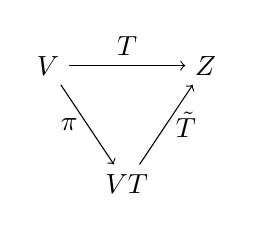
\begin{tikzpicture}
		\node (V) at (-1,1.5) {$V$};
		\node (Z) at (1,1.5) {$Z$};
		\node (K) at (0,0) {$V\quot\Ker T$};
		\draw [->] (V) to node[above]{$T$} (Z);
		\draw [->] (V) to node[left]{$\pi$} (K);
		\draw [->] (K) to node[right]{$\tilde{T}$} (Z);
	\end{tikzpicture}
\end{figure}
\begin{proof}
	L'applicazione $\tilde{T}$ è naturalmente definita come $\tilde{T}(\Ker T+x)=T(x)$.

	Verifichiamo innanzitutto che l'applicazione $\tilde{T}$ sia \emph{ben definita}, ossia che $\tilde{T}(X)$ non dipenda dal rappresentante scelto per la classe	$X$.
	Sia $\Ker T+x\in V\quot\Ker T$, e prendiamo un altro rappresentante $y\in V$, tale che $\Ker T+x=\Ker T+y$: le immagini delle due classi dovranno coincidere.
	Dato che $x\sim y$, risulta $x-y\in\Ker T$, ma allora $\tilde{T}(\Ker T+x)-\tilde{T}(\Ker T+y)=T(x)-T(y)=T(x-y)=0_Z$ cioè $\tilde{T}(\Ker T+x)=\tilde{T}(\Ker T+y)$.
	Analogamente, se per un $w\in V$ si avesse $\Ker T+x\ne\Ker T+w$, allora anche $\tilde{T}(\Ker T+x)\ne\tilde{T}(\Ker T+w)$: è sufficiente notare che se, per assurdo, le immagini coincidessero, allora dovrebbero coincidere anche le preimmagini, poich\'e risulterebbe $x-w\in\Ker T$.
	Quindi l'applicazione è ben definita.

	L'unicità è immediata: supponiamo che esista un'altra applicazione $U\colon V\quot\Ker T\to Z$ tale che $U\big(\pi(x)\big)=T(x)$.
	Per ogni $y\in V\quot\Ker T$ esiste $x\in V$ tale per cui $\pi(x)=y$, dunque $U(y)=U\big(\pi(x)\big)=T(x)=\tilde{T}\big(\pi(x)\big)=\tilde{T}(y)$, ma allora $U=\tilde{T}$.

	Mostriamo ora che è lineare, rispetto alle operazioni nello spazio quoziente introdotte nella sezione \ref{sec:spazi_quoziente}.
	Prendiamo $\Ker T+a,\Ker T+b\in V\quot\Ker T$ e $\lambda\in K$: risulta
	\begin{multline}
		\tilde{T}\big((\Ker T+a)+\lambda(\Ker T+b)\big)=\tilde{T}\big(\!\Ker T+(a+\lambda b)\big)=T(a+\lambda b)=\\=T(a)+\lambda T(b)=\tilde{T}(\Ker T+a)+\lambda\tilde{T}(\Ker T+b)
	\end{multline}
	perciò $\tilde{T}$ è lineare.

	Il nucleo di $\tilde{T}$ è $\Ker\tilde{T}=\{\Ker T+v\in V/\Ker T\colon T(v)=0_Z\}$.
	Ma se $T(v)=0_Z$ allora $v\in\Ker T$, perciò $\Ker T+v=\Ker T+0_V$ ossia $\Ker\tilde{T}=\{\Ker T+0_V\}$: ciò prova che $\tilde{T}$ è iniettiva.

	Se infine prendiamo l'applicazione $T$ solo tra $V$ e la sua immagine $T(V)$, è ovviamente suriettiva.
	Possiamo quindi trovare un'unica applicazione $L\colon V\quot\Ker T\to T(V)$ sfruttando quanto dimostrato finora.
	Se $z\in T(V)$ allora esiste $v\in V$ tale che $T(v)=z$, dunque è sufficiente prendere $a=\Ker T+v$ per ottenere $L(a)=z$, perciò per ogni $z\in T(V)$ troviamo sempre una controimmagine in $L$: ciò prova che $L\colon V\quot\Ker T\to T(V)$ è anche suriettiva, oltre che iniettiva.
	
	Di conseguenza $L\colon V\quot\Ker T\to T(V)$ è un isomorfismo.
\end{proof}

\begin{corollario} \label{cor:nullita-rango}
	Se $V$ ha dimensione finita e $T\in\lin(V,Z)$, allora $\dim V=\dim\Ker T+\dim\Imm T$.
\end{corollario}
\begin{proof}
	Segue facilmente dal teorema precedente e dal \ref{t:dimensione-quoziente}.
\end{proof}
Da quest'ultima formula possiamo dedurre delle proprietà generali su nucleo e immagine di applicazioni vettoriali.
Se $T\in\lin(V,Z)$, distinguiamo alcuni casi.
\begin{itemize}
	\item Se $\dim V>\dim Z$, allora $T$ non può essere iniettiva, infatti $\Imm T\le Z$ implica $\dim\Imm T\le\dim Z$ da cui $\dim\Ker T=\dim V-\dim\Imm T>0$.
	\item Se $\dim V<\dim Z$, allora $T$ non può essere suriettiva, dato che $\dim\Imm T=\dim V-\dim\Ker T\le\dim V<\dim Z$ quindi non può risultare $\Imm T=Z$.
	\item Se $\dim V=\dim Z$, come è per gli endomorfismi (in cui $Z=V$), iniettività e suriettività si implicano a vicenda: se $T$ è iniettiva allora $\dim\Ker T=0$ da cui $\dim\Imm T=\dim Z$, cioè $\Imm T=Z$ quindi $T$ è suriettiva.
		Viceversa, se $T$ è suriettiva allora $\dim\Imm T=\dim Z=\dim V$ da cui $\dim\Ker T=0$ ossia $\Ker T=\{0\}$.
\end{itemize}

\begin{teorema}[Secondo teorema dell'isomorfismo]
	Siano $W,Z$ sottospazi vettoriali di $V$.
	Allora l'applicazione $T\colon (W+Z)\quot Z\to W\quot(W\cap Z)$ definita come
	\begin{equation}
		T(Z+w+z)=W\cap Z+w
	\end{equation}
	è un isomorfismo.
\end{teorema}
\begin{proof}
	Innanzitutto l'applicazione $T$ deve essere ben definita, cioè non deve dipendere dai rappresentanti della classe.
	Prendiamo due elementi $Z+w+z$ e $Z+w'+z'$ (per $z,z'\in Z$ e $w,w'\in W$) i cui rappresentanti sono in relazione tra loro, ossia tali che $w+z-w'-z'\in Z$.
	Chiaramente $z-z'\in Z$, da cui segue che $w-w'\in Z$: ma allora $w-w'\in W\cap Z$ quindi le immagini $W\cap Z+w$ e $W\cap Z+w'$ coincidono (la loro differenza è $W\cap Z+w-W\cap Z+w'=W\cap Z+(w-w')=W\cap Z$ che è l'elemento neutro dello spazio di arrivo).
	Questo prova che $T$ è ben definita.
	
	Verifichiamo che è lineare: presi $z_1,z_2\in Z$, $w_1,w_2\in W$ e $\lambda\in K$ abbiamo\footnote{Nel tornare da $W\cap Z+w$ a $Z+w+z$, la scelta dell'elemento $z$ è arbitraria, poich\'e come elementi dello spazio quoziente $Z+z=Z$ per ogni $z\in Z$, quindi possiamo scegliere proprio $z_1$ e $z_2$ per riottenere le controimmagini.}
	\begin{equation}
		\begin{split}
			T\big(Z+w_1+z_1+\lambda(Z+w_2+z_2)\big)&=T(Z+z_1+\lambda z_2+w_1+\lambda w_2)=\\
			&=W\cap Z+w_1+\lambda w_2=\\
			&=W\cap Z+w_1+\lambda(W\cap Z+w_2)=\\
			&=T(Z+w_1+z_1)+\lambda T(Z+w_2+z_2)
		\end{split}
	\end{equation}
	quindi $T$ è lineare.

	Evidentemente $T$ è suriettiva.
	Il suo nucleo è formato da quegli elementi $Z+w+z$ tali che $W\cap Z+w=0$, ossia $w\in W\cap Z$.
	Allora vale anche $w\in Z$, da cui $w+z\in Z$.
	Di conseguenza $Z+w+z=Z$, cioè è lo zero dello spazio quoziente $(W+Z)\quot Z$.
	Ciò prova che $T$ è anche iniettiva, quindi è un isomorfismo.
\end{proof}
\begin{corollario}[Formula di Grassmann]
	Se gli spazi vettoriali $W$ e $Z$ hanno dimensione finita, allora $\dim(W+Z)=\dim W+\dim Z-\dim(W\cap Z)$.
\end{corollario}
\begin{proof}
	I due spazi $(W+Z)\quot Z$ e $W\quot(W\cap Z)$ dal teorema precedente sono isomorfi, perciò hanno la stessa dimensione.
	Allora per il teorema \ref{t:dimensione-quoziente} si ha che $\dim(W+Z)-\dim Z=\dim W-\dim(W\cap Z)$, da cui la tesi.
\end{proof}

\section{Matrice associata}
\label{sec:matrice-associata}
Abbiamo visto nel capitolo precedente che per uno spazio vettoriale $V$ su un campo $K$ e di dimensione $n$, una volta scelta una base, possiamo associare ad ogni $v\in V$ un vettore in $K^n$, che contiene le sue coordinate rispetto alla base.
Studiando le applicazioni lineari su $V$ è utile quindi, in modo analogo, associare ad ogni applicazione un opportuno oggetto matematico che operi sui vettori delle coordinate.
In questo modo possiamo l'applicazione di una mappa lineare su un vettore diventa un calcolo concreto.
Prendiamo un'applicazione lineare $T\colon V\to Z$, con $V$ e $Z$ sul campo $K$, e le basi $\mathcal B=\{e_1,\dots,e_n\}$ per $V$ e $\mathcal C=\{f_1,\dots,f_m\}$ per $Z$.
Abbiamo visto che l'azione di un'applicazione lineare è univocamente determinata dalla sua azione su una base dello spazio di partenza: questo implica che $T$ è completamente descritta dalle immagini $T(e_i)$ per $i=1,\dots,n$.
Come elementi di $Z$, queste immagini dei vettori della base di $V$ si scrivono in termini della base $\mathcal C$ come combinazioni lineari\footnote{
	L'ordine degli indici nell'equazione si può capire con la notazione simbolica del prodotto tra il vettore colonna $A_{ij}$ e il ``vettore riga'' degli $f_i$.
}
\begin{equation}
	T(e_i)=\sum_{k=1}^mA_{ki}f_k=
	\begin{pmatrix}
		f_1&\cdots&f_m
	\end{pmatrix}
	\begin{pmatrix}
		A_{1i}\\
		\vdots\\
		A_{mi}
	\end{pmatrix}
\end{equation}
in cui i coefficienti $A_{1i},\dots,A_{mi}$ formano il vettore delle coordinate di $T(v)$ nella base $\mathcal C$.
Per $i$ che scorre da 1 a $n$, affiancando le colonne troviamo che
\begin{equation}
	\begin{pmatrix}
		T(e_1)&\cdots&T(e_n)
	\end{pmatrix}
	=
	\begin{pmatrix}
		f_1&\cdots&f_m
	\end{pmatrix}
	A
\end{equation}
dove abbiamo definito la matrice
\begin{equation}
	A\defeq
	\begin{pmatrix}
		A_{11}&A_{12}&\cdots&A_{1n}\\
		A_{21}&A_{22}&\cdots&A_{2n}\\
		\vdots&\vdots&\ddots&\vdots\\
		A_{m1}&A_{m2}&\cdots&A_{nm}
	\end{pmatrix}.
	\label{eq:matrice-associata}
\end{equation}
che è detta \emph{matrice associata} all'applicazione $T$, nelle basi $\mathcal B$ per $V$ e $\mathcal C$ per $Z$.
Per un generico vettore $v=\sum_{j=1}^nv_je_j\in V$ si ha allora
\begin{equation}
	T(v)=\sum_{j=1}^nv_jT(e_j)=\sum_{j=1}^n\sum_{k=1}^mv_jA_{kj}f_k
\end{equation}
ma scambiando le somme possiamo vedere questa equazione come
\begin{equation}
	T(v)=\sum_{k=1}^mf_k\sum_{j=1}^nA_{kj}v_j=
	\begin{pmatrix}
		f_1&\cdots&f_m
	\end{pmatrix}
	A
	\begin{pmatrix}
		v_1\\
		\vdots\\
		v_n
	\end{pmatrix}
	=
	\begin{pmatrix}
		f_1&\cdots&f_m
	\end{pmatrix}
	\begin{pmatrix}
		T(v)_1\\
		\vdots\\
		T(v)_m
	\end{pmatrix}
\end{equation}
da cui ricaviamo
\begin{equation}
	\begin{pmatrix}
		T(v)_1\\
		\vdots\\
		T(v)_m
	\end{pmatrix}
	=A
	\begin{pmatrix}
		v_1\\
		\vdots\\
		v_n
	\end{pmatrix}.
\end{equation}
L'azione della mappa $T$ su $v\in V$ si traduce quindi nella moltiplicazione della matrice $A$ cos\`i definita per il vettore delle coordinate $[v]_{\mathcal B}$, o in breve
\begin{equation}
	[T(v)]_{\mathcal C}=A[v]_{\mathcal B}.
\end{equation}
Ad ogni applicazione $T$ da uno spazio di dimensione $n$ a uno spazio di dimensione $m$, sul campo $K$, possiamo allora associare una matrice in $\mat(m,n,K)$.

Vediamo questo fatto in maniera rigorosa nel seguente teorema.
Anzich\'e considerare lo spazio delle applicazioni lineari tra due generici spazi $V$ e $Z$ su un campo $K$, partiremo direttamente dalle applicazioni lineari tra $K^n$ e $K^m$ (dove $n=\dim V$ e $m=\dim Z$): l'isomorfismo $\lin(K^n,K^m)\cong\lin(V,Z)$ dovrebbe risultare ovvio.
\begin{teorema} \label{t:matrice-associata}
	La mappa $T\colon\mat(m,n,K)\to\lin(K^n,K^m)$ definita da $T\colon A\to T_A$ dove $T_A$ è l'applicazione lineare
	\begin{equation}
		T_A\colon
		\begin{bmatrix}
			v_1\\
			\vdots\\
			v_n
		\end{bmatrix}
		\in K^n\to
		\begin{bmatrix}
			\sum_{i=1}^nA_{1i}v_i\\
			\vdots\\
			\sum_{i=1}^nA_{mi}v_i
		\end{bmatrix}
		\in K^m
		\label{eq:azione-applicazione-lineare-associata}
	\end{equation}
	è un'isomorfismo tra i due spazi vettoriali.
\end{teorema}
\begin{proof}
	Mostriamo innanzitutto che la mappa è lineare: date $A,B\in\mat(m,n,K)$ si ha, per il vettore $v=[v_1\,\cdots\,v_n]^T$ come nella \eqref{eq:azione-applicazione-lineare-associata},
	\begin{multline}
		T_{A+B}(v)=
		\begin{bmatrix}
			\sum_{i=1}^n(A+B)_{1i}v_i\\
			\vdots\\
			\sum_{i=1}^n(A+B)_{mi}v_i
		\end{bmatrix}
		=
		\begin{bmatrix}
			\sum_{i=1}^nA_{1i}v_i+\sum_{i=1}^nB_{1i}v_i\\
			\vdots\\
			\sum_{i=1}^nA_{mi}v_i+\sum_{i=1}^nB_{mi}v_i\\
		\end{bmatrix}
		=\\=
		\begin{bmatrix}
			\sum_{i=1}^nA_{1i}v_i\\
			\vdots\\
			\sum_{i=1}^nA_{mi}v_i
		\end{bmatrix}
		+
		\begin{bmatrix}
			\sum_{i=1}^nB_{1i}v_i\\
			\vdots\\
			\sum_{i=1}^nB_{mi}v_i
		\end{bmatrix}
		=T_A(v)+T_B(v)
		\label{eq:additivita-matrice-associata}
	\end{multline}
	perciò è additiva, e analogamente è omogenea poich\'e
	\begin{equation}
		T_{\lambda A}(v)=
		\begin{bmatrix}
			\sum_{i=1}^n(\lambda A)_{1i}v_i\\
			\vdots\\
			\sum_{i=1}^n(\lambda A)_{mi}v_i
		\end{bmatrix}
		=
		\begin{bmatrix}
			\lambda\sum_{i=1}^nA_{1i}v_i\\
			\vdots\\
			\lambda\sum_{i=1}^nA_{mi}v_i
		\end{bmatrix}
		=\lambda
		\begin{bmatrix}
			\sum_{i=1}^nA_{1i}v_i\\
			\vdots\\
			\sum_{i=1}^nA_{mi}v_i
		\end{bmatrix}
		=\lambda T_A(v).
		\label{eq:omogeneita-matrice-associata}
	\end{equation}
	Di conseguenza $T$ è lineare.

	Il nucleo di $T$ è composto dalle matrici $A\in\mat(m,n,K)$ tali che $T_A$ è l'applicazione identicamente nulla, cioè $T_A(v)=0$ $\forall v\in V$.
	Presi gli elementi $\{e_1,\dots e_n\}$ della base canonica di $K^n$ si ha allora, dato che la $j$-esima componente di $e_i$ è $(e_i)_j=\delta_{ij}$, che
	\begin{equation}
		T_A(e_k)=
		\begin{bmatrix}
			A_{1k}\\
			\vdots\\
			A_{mk}
		\end{bmatrix}
	\end{equation}
	per il $k$-esimo elemento: il vettore coincide con la $k$-esima colonna della matrice $A$.
	Se l'applicazione $T_A$ è identicamente nulla, $T_A(e_k)=0$ $\forall k\in\{1,\dots,n\}$ ma ciò significa che $A$ ha tutti gli elementi nulli, cioè $A=0$.
	Dunque $T$ è iniettiva.

	Presa ora un'applicazione lineare $L\in\lin(K^n,K^m)$, la sua azione sulla base canonica $\{e_1,\dots,e_n\}$ di $K^n$ definisce $n$ vettori di $K^m$.
	Affiancando le colonne di questi vettori costruiamo la matrice $A_L\defeq[L(e_1)\,\cdots L(e_n)]\in\mat(m,n,K)$.
	A tale matrice, attraverso la mappa $T$, associamo dunque l'applicazione lineare $T_L$ come nella \eqref{eq:azione-applicazione-lineare-associata}, ed è evidente che per ogni $k\in\{1,\dots,n\}$ si ha $L(e_k)=A_Le_k=T_L(e_k)$, per come è stata costruita $A_L$.
	Siccome $L$ e $T_L$ coincidono su una base di $K^n$, per il teorema \ref{t:unicita-applicazione-lineare} le due applicazioni coincidono su tutto $K^n$.
	Per ogni applicazione $L\in\lin(K^n,K^m)$ possiamo cos\`i individuare una matrice $A_L\in\mat(m,n,K)$ tale che $T\colon A_L\to L$, e ciò mostra che $T$ è suriettiva.

	La mappa $T$ è quindi un isomorfismo tra $\mat(m,n,K)$ e $\lin(K^n,K^m)$.
\end{proof}

\section{Composizione}
Prendiamo tre spazi vettoriali $V,W,Z$ sullo stesso campo $K$: prese due applicazioni lineari $T\colon V\to W$ e $S\colon W\to Z$, possiamo comporli (come qualunque funzione) per ottenere un'applicazione $S\circ T\colon V\to Z$, che è ancora evidentemente lineare: per $a,b\in K$ e $v_1,v_2\in V$ si ha
\begin{equation}
	(S\circ T)(av_1+bv_2)=S\big(aT(v_1)+bT(v_2)\big)=S\big(aT(v_1)\big)+S\big(bT(v_2)\big)=a(S\circ T)(v_1)+b(S\circ T)(v_2).
	\label{eq:linearita-applicazione-composta}
\end{equation}
Anche all'applicazione composta possiamo associare una matrice di $\mat(\dim Z,\dim V,K)$ come già visto.
Vediamo però come tale matrice si mette in relazione con le singole matrici di $S$ e $T$.
\begin{teorema} \label{t:matrice-applicazione-composta}
	Siano $V$, $W$ e $Z$ spazi vettoriali sul campo $K$, in cui scegliamo le basi, rispettivamente, $\{e_1,\dots,e_n\}$, $\{f_1,\dots,f_m\}$, $\{g_1,\dots,g_p\}$.
	Se $T\colon V\to W$ e $S\colon W\to Z$ sono applicazioni lineari tra gli spazi e $A_T\in\mat(m,n,K)$ e $A_S\in\mat(p,m,K)$ le matrici associate, nelle basi date, rispettivamente alle due applicazioni, allora la matrice associata a $S\circ T$ è il prodotto $A_SA_T\in\mat(p,n,K)$, sempre nelle basi scelte.
\end{teorema}
\begin{proof}
	Applicando la composizione di $S$ e $T$ all'$i$-esimo elemento della base di $V$ otteniamo una combinazione lineare
	\begin{equation}
		(S\circ T)(e_i)=\sum_{k=1}^p(A_{S\circ T})_{ki}g_k
	\end{equation}
	ma allo stesso tempo
	\begin{multline}
		S\big(T(e_i)\big)=S\bigg(\sum_{j=1}^m(A_T)_{ji}f_j\bigg)=\sum_{j=1}^m(A_T)_{ji}S(f_j)=\sum_{j=1}^m(A_T)_{ji}\sum_{k=1}^p(A_S)_{kj}g_k=\sum_{k=1}^p\sum_{j=1}^m(A_S)_{kj}(A_T)_{ji}g_k.
	\end{multline}
	Per l'unicità della matrice associata si ha cos\`i
	\begin{equation}
		(A_{S\circ T})_{ki}=\sum_{j=1}^m(A_S)_{kj}(A_T)_{ji}
	\end{equation}
	che è il prodotto riga per colonna, in ordine, $A_SA_T$.
\end{proof}
Abbiamo visto che lo spazio $\End(V)$ delle applicazioni lineari da $V$ (sul campo $K$, con $\dim V=n$) a s\'e stesso è un'algebra: quest'ultimo teorema mostra in aggiunta che la mappa che associa a una matrice, in questo caso quadrata, $\mat(n,K)$ un'applicazione $T\in\End(V)$ (come nella \eqref{eq:azione-applicazione-lineare-associata}) preserva anche l'operazione di composizione, vale a dire che la composizione di due applicazioni corrisponde al prodotto delle matrici associate.
La matrice associata all'applicazione identità di $V$ è, in qualsiasi base, inoltre la matrice $n\times n$ diagonale
\begin{equation}
	I=
	\begin{bmatrix}
		1&0&\cdots&0\\
		0&1&\cdots&0\\
		\vdots&\vdots&\ddots&\vdots\\
		0&0&\cdots&1
	\end{bmatrix}
\end{equation}
ossia $I_{ij}=\delta_{ij}$, che è l'elemento neutro di $\mat(n,K)$.
In altre parole, ciò mostra l'isomorfismo \emph{tra algebre} $\mat(n,K)\cong\End(V)$.

\section{Inversione}
Guardiamo ora al problema di determinare quando un'applicazione è invertibile.
Prendiamo due spazi vettoriali $V$ e $Z$ sul campo $K$ e un'applicazione lineare $T\colon V\to Z$.
Come una qualsiasi funzione, $T$ è invertibile se e solo se è iniettiva, quindi in questo caso se $\Ker T=\{0\}$.
Se anche $\Ker T\ne\{0\}$ possiamo invertire $T$ restringendo il suo dominio a un sottospazio di $V$ che non comprenda $\Ker T$.

Prendiamo invece lo spazio degli endomorfismi di $V$, a ciascuno dei quali possiamo associare una matrice quadrata $n\times n$ ($n=\dim V$).
In questo caso sappiamo quando tale matrice è invertibile, ossia se esiste una matrice (sempre $n\times n$) $B$ tale che $AB=BA=I$.
Nel seguente teorema vediamo come questa condizione si collega all'invertibilità della corrispondente applicazione lineare: ricordiamo che, essendo un endomorfismo, se è iniettivo è anche suriettivo, dunque è un isomorfismo.
\begin{teorema} \label{t:invertibilita-matrice-associata}
	Sia $T\in\End(V)$ e $A_T$ la sua matrice associata, nella stessa base in partenza e in arrivo.
	La matrice $A_T$ è invertibile se e solo se $T$ è un isomorfismo.
\end{teorema}
\begin{proof}
	Sia $T$ un isomorfismo, cioè invertibile: esiste quindi $T^{-1}\in\End(V)$; prendiamo le rispettive matrici associate $A_T,A_{T^{-1}}\in\mat(n,K)$, dove $K$ è il campo dello spazio vettoriale $V$ e $n$ la sua dimensione.
	Poich\'e $T^{-1}\circ T=T\circ T^{-1}=\id_V$, l'applicazione identità di $V$, per il teorema \ref{t:matrice-applicazione-composta} si ha
	\begin{equation}
		I=A_TA_{T^{-1}}=A_{T^{-1}}A_T
	\end{equation}
	cioè, per definizione, $A_T$ è invertibile, e inoltre $A_{T^{-1}}=A_T^{-1}$.

	Viceversa, sia ora $A_T$ invertibile: alla sua inversa $A_T^{-1}$ possiamo associare un'applicazione lineare $L$ tale che
	\begin{equation}
		L(e_i)=\sum_{k=1}^n(A_T^{-1})_{ki}e_k
	\end{equation}
	dove $\{e_1,\dots,e_n\}$ è la base di $V$.
	Allora l'applicazione $L\circ T$ è tale che
	\begin{equation}
		(L\circ T)(e_i)=\sum_{k=1}^n(A_T)_{ki}L(e_k)=\sum_{k=1}^n\sum_{j=1}^n(A_T)_{ki}(A_T^{-1})_{jk}e_j=\sum_{j=1}^n\delta_{ji}e_j=e_i
	\end{equation}
	dato che
	\begin{equation}
		\sum_{k=1}^n(A_T^{-1})_{jk}(A_T)_{ki}=\delta_{ji}
	\end{equation}
	essendo le due matrici l'una l'inversa dell'altra, cioè $(A_T^{-1}A_T)_{ji}=I_{ji}=\delta_{ji}$.
	Abbiamo trovato quindi che $L\circ T=\id_V$, e analogamente si mostra che $T\circ L=\id_V$.
	Ciò prova che l'inverso di $T$ esiste (è $L$), cioè che $T$ è un isomorfismo.
\end{proof}
Un endomorfismo invertibile è detto \emph{automorfismo}, e l'insieme degli automorfismi di uno spazio $V$ si indica con $\Aut(V)$.
Non entreremo ora nei dettagli su come costruire l'applicazione inversa: per farlo ci serve la teoria dei determinanti, che vedremo in seguito.
\section{Cambiamento di base}
\label{sec:cambiamento-base}
Prendiamo due basi $\mathcal B=\{e_1,\dots,e_n\}$ e $\tilde{\mathcal B}=\{\tilde e_1,\dots\tilde e_n\}$ in uno spazio vettoriale $V$ di dimensione $n$, finita.
Vogliamo studiare in questa sezione come cambiano i vettori delle coordinate e le matrici associate passando da una base all'altra.
Gli elementi della base $\tilde{\mathcal B}$, essendo elementi di $V$, si scrivono a loro volta come combinazione lineare nella base $\mathcal B$: per ogni $\tilde e_i$ esistono dei coefficienti $L_{ik}$ tali che
\begin{equation}
	\tilde e_i=\sum_{k=1}^nL_{ik}e_k=
	\begin{pmatrix}
		e_1&\cdots&e_n
	\end{pmatrix}
	\begin{pmatrix}
		L_{i1}\\
		\vdots\\
		L_{in}
	\end{pmatrix}.
\end{equation}
Affiancando tutti gli elementi della base $\tilde{\mathcal B}$ scriviamo allora che
\begin{equation}
	\begin{pmatrix}
		\tilde e_1&\cdots&\tilde e_n
	\end{pmatrix}
	=
	\begin{pmatrix}
		e_1&\cdots&e_n
	\end{pmatrix}
	L
	\label{eq:trasformazione-base}
\end{equation}
dove $L$ è la matrice
\begin{equation}
	\begin{pmatrix}
		L_{11}&\cdots&L_{n1}\\
		\vdots&\ddots&\vdots\\
		L_{1n}&\cdots&L_{nn}
	\end{pmatrix}
\end{equation}
la cui $j$-esima colonna contiene le coordinate nella base $\mathcal B$ del vettore $\tilde e_j$ della nuova base.
Tale matrice è associata, chiaramente, a un isomorfismo, poich\'e tutte le sue colonne sono linearmente indipendenti (sono una base per definizione) dunque essendo un endomorfismo iniettivo è automaticamente anche suriettivo; $L$ è dunque sempre invertibile.

Prendiamo ora un vettore $v\in V$, che scriviamo come combinazione lineare $\sum_{k=1}^nv_ke_k$ nella base $\mathcal B$ o anche, simbolicamente, con
\begin{equation}
	\begin{pmatrix}
		e_1&\cdots&e_n
	\end{pmatrix}
	\begin{pmatrix}
		v_1\\
		\vdots\\
		v_n
	\end{pmatrix}.
	\label{eq:vettore-coordinate-base-originale}
\end{equation}
Nell'altra base $\tilde{\mathcal B}$, esisteranno dei coefficienti $\tilde v_k$ tali che
\begin{equation}
	v=\sum_{k=1}^n\tilde v_k\tilde e_k=
	\begin{pmatrix}
		\tilde e_1&\cdots&\tilde e_n
	\end{pmatrix}
	\begin{pmatrix}
		\tilde v_1\\
		\vdots\\
		\tilde v_n
	\end{pmatrix},
\end{equation}
perciò usando la \eqref{eq:trasformazione-base} abbiamo
\begin{equation}
	v=
	\begin{pmatrix}
		\tilde e_1&\cdots&\tilde e_n
	\end{pmatrix}
	\begin{pmatrix}
		\tilde v_1\\
		\vdots\\
		\tilde v_n
	\end{pmatrix}=
	\begin{pmatrix}
		e_1&\cdots&e_n
	\end{pmatrix}
	L
	\begin{pmatrix}
		\tilde v_1\\
		\vdots\\
		\tilde v_n
	\end{pmatrix}
\end{equation}
da cui ricaviamo, uguagliandola alla \eqref{eq:vettore-coordinate-base-originale},
\begin{equation}
	\begin{pmatrix}
		v_1\\
		\vdots\\
		v_n
	\end{pmatrix}
	=L
	\begin{pmatrix}
		\tilde v_1\\
		\vdots\\
		\tilde v_n
	\end{pmatrix}
	\qqq
	\begin{pmatrix}
		\tilde v_1\\
		\vdots\\
		\tilde v_n
	\end{pmatrix}
	=L^{-1}
	\begin{pmatrix}
		v_1\\
		\vdots\\
		v_n
	\end{pmatrix}
	\label{eq:cambiamento-base-vettori-coordinate}
\end{equation}
dunque se $L$ è la matrice che porta la base $\mathcal B$ nella base $\tilde{\mathcal B}$ (secondo la \eqref{eq:trasformazione-base}) allora i vettori delle coordinate si trasformano con l'inversa della matrice, ossia $[v]_{\tilde{\mathcal B}}=L^{-1}[v]_{\mathcal B}$.
Si dice in questo caso che i vettori sono \emph{contravarianti}, poich\'e cambiano in modo ``contrario'' a come cambia la base.

Sia ora $T\colon V\to Z$ un'applicazione lineare, con $V$ di dimensione $n$ e $Z$ di dimensione $m$, definiti sul medesimo campo $K$.
Siano $\mathcal B,\tilde{\mathcal B}$ due basi di $V$ e $\mathcal C,\tilde{\mathcal C}$ due basi di $Z$.
Sia $A\in\mat(m,n,K)$ la matrice associata a $T$ nelle due basi $\mathcal B$ e $\mathcal C$, ossia tale che per $v\in V$
\begin{equation}
	[T(v)]_{\mathcal C}=A[v]_{\mathcal B}.
	\label{eq:matrice-associata-base-originale}
\end{equation}
Se $\tilde A$ è associata a $T$ nelle altre due basi, si ha equivalentemente
\begin{equation}
	[T(v)]_{\tilde{\mathcal C}}=\tilde A[v]_{\tilde{\mathcal B}}.
	\label{eq:matrice-associata-base-trasformata}
\end{equation}
Se ora $L$ è la matrice che porta la base $\mathcal B$ nella $\tilde{\mathcal B}$ e $M$ la matrice che porta $\mathcal C$ in $\tilde{\mathcal C}$ (come nella \eqref{eq:trasformazione-base}) allora sappiamo dalla \eqref{eq:cambiamento-base-vettori-coordinate} che
\begin{equation}
	L[v]_{\tilde{\mathcal B}}=[v]_{\mathcal B}
	\hspace{1cm}\text{e}\hspace{1cm}
	M[T(v)]_{\tilde{\mathcal C}}=[T(v)]_{\mathcal C}
\end{equation}
dunque inserendole nella \eqref{eq:matrice-associata-base-originale} troviamo
\begin{equation}
	M[T(v)]_{\tilde{\mathcal C}}=AL[v]_{\tilde{\mathcal B}}
	\qqq
	[T(v)]_{\tilde{\mathcal C}}=M^{-1}AL[v]_{\tilde{\mathcal B}}
\end{equation}
e per confronto con la \eqref{eq:matrice-associata-base-trasformata} nelle nuove basi otteniamo
\begin{equation}
	\tilde A=M^{-1}AL
	\label{eq:trasformazione-matrice-associata}
\end{equation}
che dà la matrice associata a $T$ nelle basi $\tilde{\mathcal B}$ in partenza e $\tilde{\mathcal C}$ in arrivo a partire dalla matrice associata nelle basi originarie $\mathcal B$ e $\mathcal C$.
In particolare, se $T\in\End(V)$, e scegliamo la stessa base sia in partenza che in arrivo, abbiamo che $\tilde A=L^{-1}AL$ è la matrice associata a $T$ nella nuova base.
Le matrici associate a un endomorfismo in basi differenti sono quindi tutte matrici simili.

Come esempio, prendiamo in $\R^2$ la base canonica $\mathcal B$ e la base
\begin{equation}
	\tilde{\mathcal B}=\left\{
		\begin{bmatrix}
			0\\
			-2
		\end{bmatrix},
		\begin{bmatrix}
			1\\
			2
		\end{bmatrix}
	\right\}
\end{equation}
e l'applicazione lineare $T\colon\R^2\to\R^2$ a cui è associata nella base canonica la matrice
\begin{equation}
	A=
	\begin{pmatrix}
		5&0\\
		1&4
	\end{pmatrix}.
\end{equation}
Per costruire la matrice del cambiamento di base, $L$, dobbiamo prendere le coordinate dei vettori di $\tilde{\mathcal B}$ rispetto alla base $\mathcal B$: poich\'e quest'ultima è la base canonica le coordinate coincidono con le componenti dei vettori stessi, perciò
\begin{equation}
	L=
	\begin{pmatrix}
		0&1\\
		-2&2
	\end{pmatrix}
\end{equation}
di conseguenza la matrice associata a $T$ nella base $\tilde{\mathcal B}$ (in arrivo e in partenza) è
\begin{equation}
	\tilde A=L^{-1}AL=
	\begin{pmatrix}
		1&-\frac12\\
		1&0
	\end{pmatrix}
	\begin{pmatrix}
		5&0\\
		1&4
	\end{pmatrix}
	\begin{pmatrix}
		0&1\\
		-2&2
	\end{pmatrix}
	=
	\begin{pmatrix}
		4&\frac12\\
		0&5
	\end{pmatrix}.
\end{equation}


\chapter{Spazi duali}
Tra le applicazioni lineari su uno spazio vettoriale, sono particolarmente interessanti le \emph{forme} lineari, o \emph{funzionali} lineari, ossia le applicazioni da $V$ al campo $K$ su cui è definito.
Lo spazio (anch'esso vettoriale) dei funzionali lineari è detto \emph{spazio duale} di $V$, e si indica tradizionalmente con $V^*$.
Per quanto visto nei capitoli precedenti $V^*$ è isomorfo a $\mat(1,\dim V,K)$, in quanto questi funzionali sono associati, scelta una base di $V$, a delle matrici con una sola riga: vediamo subito allora che $\dim V^*=\dim V$.

Ecco alcuni esempi importanti di funzionali lineari.
\begin{itemize}
	\item In $\R^n$, possiamo definire un iperpiano come il luogo degli zeri di una funzione
		\begin{equation*}
			f(x_1,\dots,x_n)=a_1x_1+\cdots+a_nx_n-b
		\end{equation*}
		per dei coefficienti $a_i\in\R$ non tutti nulli e $b\in\R$.
		In generale, per uno spazio vettoriale $V$ qualunque, non disponiamo di una base canonica, quindi non possiamo trovare immediatamente i coefficienti $x_1,\dots,x_n$ dell'equazione $f(x_1,\dots,x_n)=0$.
		I funzionali lineari forniscono un modo per caratterizzare gli iperpiani senza bisogno di coordinate (cioè di una base), ossia in modo \emph{canonico}.
		Possiamo interpretare l'equazione come l'applicazione di un funzionale $\alpha$ del duale di $\R^n$ sul vettore $v=[x_1\,\cdots\, x_n]^T$, ossia come $\alpha(v)=b$.
		Per un generico spazio $V$ possiamo definire un iperpiano come l'insieme $\{v\in V\colon \alpha(v)=b\}$ per un dato funzionale $\alpha\in V^*$.
	\item Nello spazio delle funzioni continue reali in $[0,1]$, una mappa da esso a $\R$ può essere ad esempio 
		\begin{equation*}
			f\mapsto\int_0^1f(t)\,\dd t
		\end{equation*}
		che è evidentemente lineare.
		Possiamo definire un funzionale lineare anche a partire dalle funzioni stesse di $\cont{}\big([0,1]\big)$: ad una funzione $g$ di tale spazio associamo il funzionale
		\begin{equation*}
			T_g\colon f\mapsto\int_0^1f(t)g(t)\,\dd t.
		\end{equation*}
		Anche il funzionale definito precedentemente è di questo tipo, con $g=1$.
\end{itemize}

\section{Base duale}
\label{sec:base-duale}
Vediamo ora quelli che probabilmente sono i funzionali lineari più importanti di $V^*$.
Scegliamo una base $\mathcal B=\{b_1,\dots,b_n\}$ per lo spazio vettoriale $V$ sul campo $K$.
Sappiamo che un'applicazione lineare è univocamente determinata dalla sua azione su una base, dunque lo stesso vale per i funzionali lineari.
Definiamo $\beta_i\colon V\to K$ come
\begin{equation}
	\beta_i(b_j)=\delta_{ij}
	\label{eq:funzionale-coordinate}
\end{equation}
per $i,j=1,\dots,n$.
In altre parole, il funzionale $\beta_i$ ``estrae'' la $i$-esima coordinata di un vettore: se $v=\sum_{j=1}^nv_jb_j$ allora $\beta_i(v)=v_i$.

Consideriamo ora l'insieme $\mathcal B^*=\{\beta_1,\dots,\beta_n\}$: preso un qualsiasi $\alpha\in V^*$, possiamo scriverlo come combinazione lineare dei $\beta_i$ osservando che se $\alpha=\sum_{k=1}^n\alpha_k\beta_k$ allora
\begin{equation}
	\alpha(b_j)=\sum_{k=1}^n\alpha_k\beta_k(b_j)=\sum_{k=1}^n\alpha_k\delta_{kj}=\alpha_j
\end{equation}
e ciò identifica i coefficienti di $\alpha$ rispetto a $\mathcal B^*$.
Preso allora $v=\sum_{i=1}^nv_ib_i$, si ha
\begin{equation}
	\alpha(v)=\sum_{i=1}^nv_i\alpha(b_i)=\sum_{i=1}^nv_i\alpha_i
\end{equation}
e allo stesso tempo
\begin{equation}
	\sum_{i=1}^n\alpha_i\beta_i(v)=\sum_{i=1}^n\alpha_i\beta_i\bigg(\sum_{j=1}^nv_jb_j\bigg)=\sum_{i=1}^n\alpha_i\sum_{j=1}^nv_j\delta_{ij}=\sum_{i=1}^n\alpha_iv_i
\end{equation}
che coincide con la precedente.
Questo verifica che qualsiasi funzionale lineare può essere espresso come combinazione lineare dei $\beta_i$.
Inoltre, se $\sum_{i=1}^n\mu_i\beta_i=0$, cioè è il funzionale nullo, allora sulla base $\mathcal B$ risulta
\begin{equation}
	0=\sum_{i=1}^n\mu_i\beta_i(b_j)=\sum_{i=1}^n\mu_i\delta_{ij}=\mu_j
\end{equation}
per $j=1,\dots,n$ quindi $\mathcal B^*$ è anche linearmente indipendente: ciò prova che è una base di $V^*$.\footnote{
	Sapendo già che la dimensione di $V^*$ è $n$, l'indipendenza lineare di $\mathcal B^*$ sarebbe stata sufficiente a mostrare che è una base di $V^*$, ciononostante questa dimostrazione è utile per capire come individuare i coefficienti di un funzionale rispetto alla base $\mathcal B^*$.
}
\begin{definizione} \label{d:base-duale}
	Data una base $\mathcal B=\{b_1,\dots,b_n\}$ di uno spazio vettoriale $V$, la base $\{\beta_1,\dots,\beta_n\}$ di $V^*$ tale che per ogni $i,j=1,\dots,n$
	\begin{equation}
		\beta_i(b_j)=\delta_{ij}
	\end{equation}
	è detta \emph{base duale} di $\mathcal B$.
\end{definizione}
Come già visto, in questa base la $i$-esima componente di un funzionale lineare $\alpha$ è data da $\alpha(b_i)$.
Va detto che non ha senso parlare di una ``base duale di $V^*$'', dato che non è unica: ad ogni scelta di una base di $V$ corrisponde una base duale per $V^*$, a essa associata.

\chapter{Determinanti}
\section{Permutazioni} \label{sec:permutazioni}
Prima di affrontare i determinanti, abbiamo bisogno di studiare le proprietà di base delle permutazioni tra numeri naturali.
\begin{definizione} \label{d:permutazione}
	Sia $J_n$ l'insieme dei naturali consecutivi fino a $n$, ossia l'insieme $\{1,2,\dots,n\}\subset\N$.
	Una \emph{permutazione} è una mappa iniettiva $\sigma\colon J_n\to J_n$.
\end{definizione}
Una permutazione si può rappresentare ad esempio nella forma
\begin{equation*}
\sigma=\begin{pmatrix}1&2&3&4&5&\cdots&n\\50&849&23&1&9234&\cdots&k\end{pmatrix},
\end{equation*}
in cui $k\in J_n$.
La scrittura $S_n$ indica l'insieme delle permutazioni $\sigma$ da $J_n$ in sé stesso.
Poiché gli insiemi $J_n$ hanno cardinalità finita, una permutazione è automaticamente anche suriettiva.
Si indica con $\sigma^{-1}$ l'inversa di $\sigma$.
La composizione di due permutazioni $\zeta$ e $\sigma$ si indica in notazione moltiplicativa come $\zeta\sigma$.
L'insieme $(S_n,\cdot)$, delle permutazioni dei primi $n$ numeri naturali rispetto alla composizione, forma un gruppo non abeliano, detto \emph{gruppo simmetrico}.
Il suo elemento neutro è la permutazione che lascia invariati tutti gli elementi di $J_n$.
\begin{definizione} \label{d:scambio}
	Si chiama \emph{scambio}, o \emph{trasposizione}, un'operazione $J_n\to J_n$ che consiste nello scambio di due elementi, lasciando invariati tutti gli altri.
\end{definizione}
L'importanza delle trasposizioni sta nella seguente proprietà.
\begin{proprieta} \label{pr:permutazione-prodotto-scambi}
	Ogni permutazione si può sempre esprimere come prodotto di scambi:
	\begin{equation*}
		\sigma=\tau_1\tau_2\cdots\tau_s.
	\end{equation*}
\end{proprieta}
\begin{proprieta} \label{pr:segno}
	Esiste ed è unica un'applicazione $\epsilon\colon S_n\to\{-1,1\}$ tale che
	\begin{itemize}
		\item se $\tau$ è uno scambio, $\epsilon(\tau)=-1$;
		\item se $\sigma_1,\sigma_2\in S_n$, allora $\epsilon(\sigma_1\sigma_2)=\epsilon(\sigma_1)\epsilon(\sigma_2)$.
	\end{itemize}
\end{proprieta}
Una tale applicazione è detta \emph{segno}.
Presa una permutazione $\sigma\in S_n$, essa si dice pari se il suo segno è 1, dispari se è $-1$.
Se $s$ è il numero di scambi effettuati, il segno della permutazione che risulta dalla loro composizione è $\epsilon(\sigma)=(-1)^s$.

\section{Applicazioni multilineari alternanti}
\begin{definizione} \label{d:applicazione-multilineare-alternante}
	Siano $V_1,V_2,\dots,V_n,W$ spazi vettoriali sul campo $K$.
	L'applicazione $T\colon V_1\times V_2\times\dots\times V_n\to W$ si dice \emph{multilineare} se $\forall v_1\in V_1,v_2\in V_2,\dots,v_n\in V_n$ e $v_i',v_i''\in V_i$ e $\mu,\lambda\in K$ si ha che
	\begin{multline*}
		T(v_1,\dots,v_{i-1},\mu v_i'+\lambda v_i'',v_{i+1},\dots,v_n)=\mu T(v_1,\dots,v_{i-1},v_i',v_{i+1},\dots,v_n)+\\+\lambda T(v_1,\dots,v_{i-1},v_i'',v_{i+1},\dots,v_n).
	\end{multline*}
	In pratica essa è lineare in ciascuna delle variabili.
	Si dice inoltre \emph{alternante} se ogniqualvolta esistono due indici $i,j\in\{1,\dots,n\}$ per i quali $v_i=v_j$, allora $T(v_1,\dots,v_i,\dots,v_j,\dots,v_n)=0$.
\end{definizione}
Dall'alternanza dell'applicazione ricaviamo subito un'importante proprietà, nel caso in cui lo spazio di partenza sia il prodotto di tante copie di un unico spazio vettoriale.
A tal proposito, come è uso comune, indichiamo
\begin{equation}
	V^n\defeq\underbracket[.5pt]{V\times V\times\cdots\times V}_{n\text{volte}}.
\end{equation}
\begin{teorema} \label{t:alternante-implica-antisimmetrica}
	Sia $T\colon V^n\to W$ un'applicazione multilineare.
	Se è alternante allora è antisimmetrica.
\end{teorema}
\begin{proof}
	Scegliamo due variabili distinte uguali a $x+y$, con $x,y\in V$.
	Risulta dalla multilinearità che
	\begin{multline}
		T(x_1,\dots,x+y,\dots,x+y,\dots,x_n)=T(x_1,\dots,x,\dots,x,\dots,x_n)+T(x_1,\dots,x,\dots,y,\dots,x_n)+\\+T(x_1,\dots,y,\dots,x,\dots,x_n)+T(x_1,\dots,y,\dots,y,\dots,x_n),
	\end{multline}
	mentre l'alternanza implica che il primo membro e il primo e ultimo termine del secondo membro sono nulli.
	Di conseguenza
	\begin{equation}
		T(x_1,\dots,x,\dots,y,\dots,x_n)+T(x_1,\dots,y,\dots,x,\dots,x_n)=0
	\end{equation}
	cioè $T$ è antisimmetrica.
\end{proof}
In generale, in seguito ad uno scambio $\tau\colon\{1,\dots,n\}\to\{1,\dots,n\}$ risulta
\begin{equation}
	T(x_{\tau(1)},\dots,x_{\tau(n)})=-T(x_1,\dots,x_n).
\end{equation}
L'implicazione inversa non è sempre vera in generale: esistono infatti dei campi in cui vale $x=-x$ anche se $x\ne 0$, come $\Z_2$ in cui $1+1=0$.
Essi sono i campi con caratteristica $2$, e in tal caso evidentemente l'antisimmetria non implica l'alternanza.
Al di là di questi casi patologici, se la caratteristica del campo è diversa da 2 allora un'applicazione antisimmetrica è anche alternante e viceversa.
\begin{proprieta} \label{pr:alternante-variabili-linearmente-dipendenti}
	Se $\{x_1,\dots,x_k\}\subset V$ è un insieme linearmente dipendente in uno spazio vettoriale $V$ su un campo $K$, allora per ogni applicazione $T\colon V^k\to K$ alternante si ha $T(x_1,\dots,x_k)=0$.
\end{proprieta}
\begin{proof}
	Esprimiamo uno dei vettori come combinazione lineare dei restanti, e sfruttiamo la multilinearità di $T$: a meno di riordinamenti, supponiamo che $x_1$ si possa scrivere come combinazione lineare
	\begin{equation}
		x_1=\alpha_2x_2+\cdots+\alpha_kx_k
	\end{equation}
	per certi $\alpha_i\in K$.
	Otteniamo cos\`i
	\begin{equation}
		T(x_1,\dots,x_k)=T\bigg(\sum_{i=2}^k\alpha_ix_i,x_2,\dots,x_k\bigg)=\sum_{i=2}^k\alpha_iT(x_i,x_2,\cdots,x_k)
	\end{equation}
	ma in ciascun $T(x_i,x_2,\dots,x_k)$ c'e sempre (poich\'e $i=2,\dots,k$) una coppia di variabili uguali, perciò ognuno di questi è nullo, vale a dire $T(x_1,\dots,x_k)=0$.
\end{proof}
L'affermazione contraria, ossia che se l'insieme è linearmente indipendente allora $T(x_1,\dots,x_k)\ne~0$, vale solo se $k=\dim V$, cioè quando l'insieme è una base di $V$.

\begin{lemma}
	Sia $V$ uno spazio vettoriale di dimensione $n$ e con base $\mathcal B=\{e_1,\dots,e_n\}$, e $W$ un altro (arbitrario) spazio vettoriale, entrambi sul campo $K$.
	Dato un insieme di $n$ vettori $\{v_1,\dots,v_n\}$, ogni applicazione multilineare alternante $T\colon V^n\to W$ si può scrivere come
	\begin{equation}
		T(v_1,\dots,v_n)=\sum_{\sigma\in S_n}\sgn(\sigma)\prod_{j=1}^nv_{\sigma(j)j}T(e_1,\dots,e_n)
	\end{equation}
	dove $v_{ab}$ è la $a$-esima componente del vettore $v_b$, ossia $v_b=\sum_{i=1}^nv_{ib}e_i$.
\end{lemma}
\begin{proof}
	Scomponiamo i vettori come combinazioni lineari degli elementi di $\mathcal B$, nella forma $v_k=\sum_{k=1}^nv_{ik}e_i$ per $i=1,\dots,n$.
	Allora, sfruttando la multilinearità, otteniamo
	\begin{multline}
		T(v_1,\dots,v_n)=
		T\bigg(\sum_{i=1}^nv_{i1}e_i,\dots,\sum_{i=1}^nv_{in}e_i\bigg)=\\=
		\sum_{i=1}^n\sum_{j=1}^n\cdots\sum_{k=1}^nv_{i1}v_{j2}\cdots v_{kn}T(e_i,e_j,\dots,e_k)=
		\sum_{f\in F_n}T(e_{f(1)},\dots,e_{f(n)})\prod_{j=1}^nv_{f(j)j},
	\end{multline}
	indicando con $F_n$ l'insieme di tutte le funzioni da $\{1,\dots,n\}$ in s\'e stesso.
	Se $f\in F_n$ non è iniettiva, allora esistono $i,k\le n$ tali per cui $f(i)=f(k)$, con $i\ne k$; dato che $T$ è alternante l'addendo corrispondente a tale $f$ è nullo.
	Rimangono dunque nella somma solo le $f$ iniettive, che sono evidentemente anche suriettive.
	Tali funzioni sono proprio le permutazioni di $\{1,\dots,n\}$: di conseguenza
	\begin{equation}
		T(v_1,\dots,v_n)=\sum_{\sigma\in S_n}T(e_{\sigma(1)},\dots,e_{\sigma(n)})\prod_{j=1}^nv_{\sigma(j)j}.
	\end{equation}
	Ora, ogni permutazione di $S_n$ può essere espressa come il prodotto di un certo numero $m$ di scambi: ogni volta che applichiamo uno di questi scambi alle variabili $e_1,\dots,e_n$ il segno di $T$ cambia, perch\'e è alternante.
	In totale, dunque, $T(e_{\sigma(1)},\dots,e_{\sigma(n)})=(-1)^mT(e_1,\dots,e_n)=\sgn(\sigma)T(e_1,\dots,e_n)$ da cui ricaviamo infine
	\begin{equation}
		T(v_1,\dots,v_n)=\sum_{\sigma\in S_n}\sgn(\sigma)T(e_1,\dots,e_n)\prod_{j=1}^nv_{\sigma(j)j}.\qedhere
	\end{equation}
\end{proof}

Ci concentriamo ora sulle \emph{forme} multilineari alternanti, ossia applicazioni da $V^n$ al campo $K$.
Una loro caratteristica fondamentale è che sono univocamente determinate da un solo elemento di $K$, come vediamo nel seguente teorema.
\begin{teorema} \label{t:unicita-applicazione-multilineare-alternante}
	Sia $V$ uno spazio vettoriale sul campo $K$ con $\dim V=n$, e $\mathcal B=\{e_1,\dots,e_n\}$ una sua base.
	Per ogni $\lambda\in K$, esiste un'unica forma multilineare alternante $h\colon V^n\to K$ tale che $h(e_1,\dots,e_n)=\lambda$.
\end{teorema}
\begin{proof}
	Ci basta mostrare che
	\begin{equation}
		h\bigg(\sum_{j_1=1}^nv_{j_11}e_{j_1},\dots,\sum_{j_n=1}^nv_{j_nn}e_{j_n}\bigg)=\lambda\sum_{\sigma\in S_n}\sgn(\sigma)\prod_{k=1}^nv_{\sigma(k)k}
		\label{eq:unicita-applicazione-multilineare-alternante}
	\end{equation}
	è la forma cercata.
	L'unicità segue allora direttamente dal lemma precedente.

	Dimostriamo che è multilineare: presi i vettori $v_1,\dots,av_k'+bv_k'',\dots,v_n$ si ha
	\begin{equation}
		\begin{split}
			&h(v_1,\dots,av_k'+bv_k'',\dots,v_n)=\\
			=\,&\lambda\!\sum_{\sigma\in S_n}\sgn(\sigma)v_{\sigma(1)1}\cdots(av_{\sigma(k)k}'+bv_{\sigma(k)k}'')\cdots v_{\sigma(n)n}=\\
			=\,&\lambda a\!\sum_{\sigma\in S_n}\sgn(\sigma)v_{\sigma(1)1}\cdots v_{\sigma(k)k}'\cdots v_{\sigma(n)n}+
			\lambda b\!\sum_{\sigma\in S_n}\sgn(\sigma)v_{\sigma(1)1}\cdots v_{\sigma(k)k}''\cdots v_{\sigma(n)n}=\\
			=\,&ah(v_1,\dots,v_k',\dots,v_n)+bh(v_1,\dots,v_k'',\dots,v_n).
		\end{split}
	\end{equation}
	Per dimostrare che è alternante, notiamo che, fissato uno scambio $\tau\in S_n$, per ogni permutazione dispari $\sigma\in S_n$ esiste una permutazione pari $\pi\in A_n$ tale che $\pi\tau=\sigma$.
	Possiamo dunque suddividere il gruppo simmetrico nei due insiemi, disgiunti, $A_n$ e $\tau A_n=\{\sigma\in S_n\colon\sigma=\pi\tau,\ \pi\in A_n\}$.
	Supponiamo ora che $v_k=v_l$ per $k\ne l$.
	Detto $\tau=(kl)$, scriviamo le permutazioni dispari come $\pi\tau$, con $\pi$ pari, ottenendo
	\begin{multline}
		\lambda\!\sum_{\sigma\in S_n}\sgn(\sigma)\prod_{j=1}^nv_{\sigma(j)j}=
		\lambda\!\sum_{\pi\in A_n}\sgn(\pi)v_{\pi(1)1}\cdots v_{\pi(n)n}+\lambda\sum_{\pi\in A_n}\sgn(\pi\tau)v_{(\pi\tau)(1)1}\cdots v_{(\pi\tau)(n)n}=\\=
		\lambda\!\sum_{\pi\in A_n}v_{\pi(1)1}\cdots v_{\pi(k)k}\cdots v_{\pi(l)l}\cdots v_{\pi(n)n}-
		\lambda\!\sum_{\pi\in A_n}v_{\pi(1)1}\cdots v_{\pi(l)k}\cdots v_{\pi(k)l}\cdots v_{\pi(n)n}
	\end{multline}
	poich\'e $(\pi\tau)(k)=\pi\big(\tau(k)\big)=\pi(l)$ e viceversa $(\pi\tau)(l)=\pi(k)$.
	Abbiamo però che $v_l=v_k$, dunque $v_{\pi(l)k}=v_{\pi(l)l}$ e $v_{\pi(k)k}=v_{\pi(k)l}$, e per questo motivo i due termini coincidono, dando 0 come risultato.
	La forma cos\`i definita è allora anche alternante.
	Infine, applicandola agli elementi (ordinati) della base $\mathcal B$, si ottiene
	\begin{equation}
		h(e_1,\dots,e_n)=\lambda\!\sum_{\sigma\in S_n}\sgn(\sigma)\delta_{\sigma(1)1}\delta_{\sigma(2)2}\cdots\delta_{\sigma(n)n}
	\end{equation}
	e l'unico addendo non nullo è quello in cui $\sigma(i)=i$ $\forall i\in\{1,\dots,n\}$, ossia $\sigma$ è l'elemento neutro di $S_n$.
	Allora $h(e_1,\dots,e_n)=\lambda\delta_{11}\delta_{22}\cdots\delta_{nn}=\lambda$.
\end{proof}
Le forme multilineari alternanti sono dunque univocamente determinate dal valore $\lambda$ che esse assumono sulla $n$-upla ordinata dei vettori della base di $V$.
In altre parole, questo teorema afferma che lo spazio delle forme multilineari alternanti $V^n\to K$ e $K$ sono, come spazi vettoriali, isomorfi tramite la mappa di valutazione
\begin{equation}
	h\mapsto h(e_1,\dots,e_n).
\end{equation}
Inoltre possiamo guardare a $V^n$ (con $n=\dim V$) come allo spazio vettoriale i cui elementi sono $n$ vettori di $n$ elementi: in questa luce è facile associarlo allo spazio $\mat(n,K)$, in cui le matrici quadrate sono formate affiancando in ordine i vettori di ciascun $V$.
Alla $n$-upla ordinata $(e_1,\dots,e_n)$ di $V^n$, se $\{e_1,\dots,e_n\}$ è la base canonica di $K^n$, corrisponde in questo modo la matrice $[e_1\ \cdots\ e_n]$ che è la matrice identità di ordine $n$.
Possiamo allora considerare le forme multilineari alternanti sia su $V^n$ che su $\mat(n,K)$.
Presa una matrice $A=(a_{ij})$ scriviamo cos\`i
\begin{equation}
	h(A)=\lambda\!\sum_{\sigma\in S_n}\sgn(\sigma)\prod_{j=1}^na_{\sigma(j)j}.
	\label{eq:forma-multilineare-alternante-matrici}
\end{equation}
\begin{definizione} \label{d:determinante}
	Definiamo \emph{determinante} di una matrice quadrata $A\in\mat(n,K)$ la forma multilineare alternante $h\colon\mat(n,K)\to K$ tale per cui $h(I_n)=1$, dove $I_n$ è la matrice identità di ordine $n$.
\end{definizione}
Il determinante di una matrice si indica solitamente con
\begin{equation}
	\det(A)\quad\text{oppure}\quad
	\begin{vmatrix}
		a_{11}&\cdots&a_{1n}\\
		\vdots&\ddots&\vdots\\
		a_{n1}&\cdots&a_{nn}
	\end{vmatrix}.
\end{equation}
Per $\lambda=1$ nella \eqref{eq:forma-multilineare-alternante-matrici} otteniamo dunque l'equazione nota come \emph{formula di Leibniz}
\begin{equation}
	\det(A)=\sum_{\sigma\in S_n}\sgn(\sigma)\prod_{j=1}^na_{\sigma(j)j}.
	\label{eq:determinante-leibniz}
\end{equation}

\paragraph{Assiomi di definizione del determinante}
Sia $\mat(n,K)$ l'insieme delle matrici quadrate di ordine $n$ e a coefficienti in un campo $K$.
Cerchiamo una funzione $\det\colon\mat(n,K)\to K$ aventi le seguenti proprietà\footnote{Nei seguenti punti si indicheranno con $A_i$ i vettori colonna di $K^n$: affiancando $n$ di questi vettori si ottiene una matrice di $\mat(n,K)$.}:
\begin{enumerate}[label=(\roman*)]
	\item $\det I=1$, dove $I$ è la matrice identità di $\mat(n,K)$;
	\item se $A$ ha due righe o colonne uguali, $\det A=0$,
		\begin{equation*}
		\det(A_1\cdots A_n)=0\text{ se }\exists i,j=1,\dots,n\colon A_i=A_j;
		\end{equation*}
	\item se $B$ è ottenuta moltiplicando una riga o una colonna di $A$ per uno scalare $k\in K$, allora $\det B=k\det A$,
		\begin{equation*}
		\det(A_1\cdots\lambda A_i\cdots A_n)=\lambda\det(A_1\cdots A_i\cdots A_n);
		\end{equation*}
	\item se $B$ è ottenuta scambiando due righe o due colonne di $A$, allora $\det B=-\det A$,
		\begin{equation*}
		\det(A_1\cdots A_i\cdots A_j\cdots A_n)=-\det(A_1\cdots A_j\cdots A_i\cdots A_n),\text{ con }i\neq j;
		\end{equation*}
	\item $\det(A_1\cdots A_i+C\cdots A_n)=\det(A_1\cdots A_i\cdots A_n)+\det(A_1\cdots C\cdots A_n);$ 
\end{enumerate}
Una funzione che soddisfa queste proprietà esiste, ed è unica, ed è appunto il determinante.

\section{Riduzione a scala}
\begin{definizione}
	Una matrice si dice \emph{ridotta a scala} se il primo termine non nullo di ciascuna riga si trova ``più a destra'' di quello della riga precedente.
	Il primo termine non nullo di una riga è detto \emph{pivot}.
\end{definizione}
La definizione vale per qualsiasi tipo di matrice; ora ci concentriamo su quelle quadrate, per le quali è definito il determinante.
Per tali matrici, essere ridotta a scala significa essere triangolare superiore: tutti gli elementi sotto la diagonale sono nulli.
\begin{proprieta}[Metodo di Gauss]
	Sia $K$ un campo con caratteristica\footnote{
		La caratteristica di $K$ è il più piccolo numero naturale $n$ tale che $nx=0$ per ogni elemento $x$ di $K$: $\cha K=\{n\in\N\colon nx=0_K,\ \forall x\in K\}$. Se tale numero non esiste, la caratteristica è per definizione 0.
	}
	diversa da 2.
	Sia $\det\colon\mat(n,K)\to K$ una funzione soddisfacente le proprietà precedentemente elencate.
	Allora:
	\begin{enumerate}
		\item Se $A$ ha una riga o una colonna nulla, $\det A=0$.
		\item Per $\lambda,\mu\in K$, se $A_i'=\lambda A_i+\mu A_j$, dove $\{A_k\}_{k=1}^n$ indicano le righe della matrice, allora
		\begin{equation*}
			\begin{vmatrix}
				A_1\\A_i'\\A_j\\A_n
			\end{vmatrix}
			=\lambda
			\begin{vmatrix}
				A_1\\A_i\\A_j\\A_n
			\end{vmatrix}.
		\end{equation*}
		\item Se $\rk A<n$, dove $n$ è l'ordine della matrice, allora $\det A=0$; se invece $\rk A=n$, $\det A=(-1)^sp_1p_2\cdots p_n$, dove $s$ è il numero di scambi di righe o colonne effettuati e $p_1,\dots,p_n$ sono i pivot della matrice ridotta a scala.
	\end{enumerate}
\end{proprieta}
\begin{proof}
	\begin{enumerate}
	\item La riga o colonna nulla si può vedere come $0\cdot A_i$ dove $A_i$ è una riga o colonna qualunque, quindi per la (iii) si ha che il determinante è nullo.
	\item Per la (v) si ha
		\begin{equation*}
			\begin{vmatrix}
				A_1\\\vdots\\\lambda A_i+\mu A_j\\ A_j\\\vdots\\A_n
			\end{vmatrix}
			=
			\begin{vmatrix}
				A_1\\\vdots\\\lambda A_i\\ A_j\\\vdots\\A_n
			\end{vmatrix}
			+
			\begin{vmatrix}
				A_1\\\vdots\\\mu A_j\\ A_j\\\vdots\\A_n
			\end{vmatrix}
			=\lambda
			\begin{vmatrix}
				A_1\\\vdots\\A_i\\ A_j\\\vdots\\A_n
			\end{vmatrix}
			+\mu
			\begin{vmatrix}
				A_1\\\vdots\\A_j\\ A_j\\\vdots\\A_n
			\end{vmatrix},
		\end{equation*}
		ma la seconda matrice ha due righe uguali quindi il suo determinante è nullo per il punto precedente.
	\item Per ridurre a scala una matrice, si cambia il segno del determinante tante volte ($s$) quante volte si sono scambiate due righe, mentre il determinante non varia sostituendo ad una riga $A_i$ una combinazione lineare del tipo $1_KA_i+\mu A_j$, con $i\neq j$.
		Se il rango della matrice non è massimo, cioè non è esattamente $n$, si ha automaticamente come risultato una riga nulla, quindi il determinante è nullo.
		Altrimenti, sia
		\begin{equation*}
			B=
			\begin{pmatrix}
				b_{11}	&b_{12}	&\dots	&b_{1n}\\
				0		&b_{22}	&\dots 	&b_{2n}\\
				\vdots 	&\vdots 	&\ddots 	&\vdots\\
				0		&0		&\dots 	&b_{nn}
			\end{pmatrix}.
		\end{equation*}
		Si può scrivere la prima riga come la somma dei vettori riga $B_1=B_1'+B_1''$, dove $B_1'=(b_{11},0,\dots,0)$ e $B_1''=(0,b_{12},\dots,b_{1n})$.
		Allora risulta
		\begin{equation*}
			\det B=
			\begin{vmatrix}
				B_1'\\\vdots\\B_n
			\end{vmatrix}
			+
			\begin{vmatrix}
				B_1''\\\vdots\\B_n
			\end{vmatrix},
		\end{equation*}
		ma il secondo termine ha la prima colonna nulla, ossia il suo rango non è massimo, perciò ha determinante nullo.
		Iterando il processo sulle righe seguenti, si ottiene che il determinante di $B$ è uguale al determinante della matrice diagonale
		\begin{equation*}
			\begin{pmatrix}
				b_{11}	&0		&\dots	&0\\
				0		&b_{22}	&\dots	&0\\
				\vdots 	&\vdots	&\ddots	&\vdots\\
				0		&0		&\dots	&b_{nn}
			\end{pmatrix},
		\end{equation*}
		che è a sua volta equivalente a $b_{11}b_{22}\cdots b_{nn}$, si ha quindi $\det B=b_{11}b_{22}\cdots b_{nn}$.
	\end{enumerate}
\end{proof}

Andiamo ora a vedere le condizioni che permettono a una matrice di essere ridotta a scala:
\begin{proprieta} \label{pr:pivot-riduzione-scala}
	Una matrice generica $A$ può essere ridotta a scala se soddisfa le seguenti proprietà:
	\begin{itemize}
		\item Se $A_{ij}$ è la riga e la colonna in cui la matrice $A$ ammette un pivot, allora la $i$-esima riga, se ammette un pivot, lo ammette su una colonna di indice almeno $j+1$.
		\item Se la riga $j$-esima di $A$ non ammette pivot, allora non li ammette nemmeno la riga $j+1$-esima.
	\end{itemize}
\end{proprieta}
\begin{definizione}
	Sia $A$ una matrice, si definisce \emph{rango} di $A$ il numero di pivot della sua riduzione a scala.
	Esso si indica con $\rk A$.
\end{definizione}
Diamo ora senza dimostrazione due teoremi importanti per i sistemi lineari.
\begin{teorema}[di Cramer] \label{t:cramer}
	Sia $A\in\mat(n,K)$: se $\rk A=n$ allora per ogni $b\in K^n$ il sistema lineare composto da $A$, detta matrice dei coefficienti, e da $b$, vettore dei termini noti, ammette una ed una sola soluzione.
\end{teorema}
Per dimostrarlo è sufficiente considerare la matrice $A\mid b$ e ridurla a scala.
\begin{teorema}[di Rouch\'e-Capelli] \label{t:rouche-capelli}
	Sia $A\in\mat(n,K)$ e sia $b\in K^n$, se $A$ è la matrice dei coefficienti e $b$ il vettore dei termini noti.
	Allora:
	\begin{enumerate}
		\item Il sistema ammette soluzioni se e solo se $\rk A=\rk(A\mid b)$.
		\item Se il sistema ammette soluzioni, allora l'insieme delle soluzioni dipende dal numero delle incognite e dal rango (cioè $n$ e $\rk A$).
	\end{enumerate}
\end{teorema}

\section{Calcolo del determinante}
Il determinante coincide in pratica con la somma di tutti i possibili prodotti tra elementi di righe e colonne diverse della matrice: questa definizione è ovviamente inutilizzabile in generale, ma per le matrici di ordini piccoli si traduce in formule veloci per il suo calcolo.
Il determinante di una matrice nulla è ovviamente 0.
Per le matrici di ordine 1, che sono gli scalari del campo $K$, il determinante coincide con la loro unica componente: $\det(k_{11})=k_{11}$.
Per le matrici di ordine 2 vale
\begin{equation*}
	\det
	\begin{pmatrix}
		a&b\\c&d
	\end{pmatrix}
	=ad-bc.
\end{equation*}
Per le matrici di ordine 3 si può utilizzare la \emph{regola di Sarrus}: il determinante può essere espresso come la somma dei prodotti degli elementi sulle tre ``diagonali'' a cui si sottrae la somma dei prodotti di quelli sulle ``antidiagonali'':
\begin{equation*}
	\det
	\begin{pmatrix}
		a_{11}&a_{12}&a_{13}\\
		a_{21}&a_{22}&a_{23}\\
		a_{31}&a_{32}&a_{33}
	\end{pmatrix}
	=a_{11}a_{22}a_{33}+a_{12}a_{23}a_{31}+a_{13}a_{21}a_{32}-a_{11}a_{23}a_{32}-a_{12}a_{21}a_{33}-a_{13}a_{22}a_{31}.
\end{equation*}
Tale regola \emph{non} si può estendere a matrici di ordini superiori.

\begin{teorema}[Formula di Leibnitz] \label{t:determinante-leibnitz}
	Sia $A=(a_{ij})\in\mat(n,K)$, con $\cha K\neq 2$.
	Il suo determinante è dato da
	\begin{equation}\label{eq:determinante-leibnitz}
		\det A=\sum_{\sigma\in S_n}\epsilon(\sigma)\prod_{i=1}^na_{i\sigma(i)}.
	\end{equation}
\end{teorema}
\begin{proof}
	Sia $\{e_j\}_{j=1}^n$ la base canonica di $K^n$.
	Si può scrivere $A$ come
	\begin{equation*}
		A=
		\begin{pmatrix}
			A_1\\A_2\\\vdots\\A_n
		\end{pmatrix}
		=
		\begin{pmatrix}
			a_{11}e_1+\dots+a_{1n}e_n\\
			a_{21}e_1+\dots+a_{2n}e_n\\
			\vdots\\
			a_{n1}e_1+\dots+a_{nn}e_n
		\end{pmatrix}.
	\end{equation*}
	Il suo determinante è la somma di elementi del tipo
	\begin{equation*}
		\det
		\begin{pmatrix}
			a_{1\sigma(1)}e_{\sigma(1)}\\
			\vdots\\
			a_{n\sigma(n)}e_n
		\end{pmatrix},
	\end{equation*}
	per linearità, scomponendo il determinante per ogni riga.
	Quindi
	\begin{equation*}
		\det
		\begin{pmatrix}
			a_{1\sigma(1)}e_{\sigma(1)}\\
			\vdots\\
			a_{n\sigma(n)}e_{n\sigma(n)}
		\end{pmatrix}
		=a_{1\sigma(1)}\cdots a_{n\sigma(n)}\det
		\begin{pmatrix}
			e_{\sigma(1)}\\
			\vdots\\e_{n\sigma(n)}
		\end{pmatrix}.
	\end{equation*}
	Sempre per la linearità, tutti questi determinanti si possono sommare, ottenendo
	\begin{equation*}
		\begin{split}
			\det A&=\sum_{\sigma\in S_n}a_{1\sigma(1)}\cdots a_{n\sigma(n)}\det\begin{pmatrix}e_{\sigma(1)}\\\vdots\\e_{\sigma(n)}\end{pmatrix}=\\
			&=\sum_{\sigma\in S_n}a_{1\sigma(1)}\cdots a_{n\sigma(n)}\epsilon(\sigma)\det\begin{pmatrix}e_1\\\vdots\\e_n\end{pmatrix}=\\
			&=\sum_{\sigma\in S_n}\epsilon(\sigma)a_{1\sigma(1)}\cdots a_{n\sigma(n)}.\qedhere
		\end{split}
	\end{equation*}
\end{proof}

Anche il metodo di Leibnitz, però, non fa molta luce su come si dovrebbe calcolare il determinante.
Il metodo più usato è la \emph{scomposizione di Laplace} per righe o per colonne.
\begin{definizione} \label{d:minori-complementi}
	Siano $A\in\mat(n,K)$ e $i,k\in\{1,\dots,n\}$.
	Con $A_{ik}$ si indica la sottomatrice ottenuta eliminando da $A$ la riga $i$-esima e la colonna $k$-esima.
	Si definiscono:
	\begin{itemize}
		\item \emph{minore complementare} dell'elemento $a_{ik}$ di $A$ la quantità $M_{ik}=\det A_{ik}$;
		\item \emph{complemento algebrico}, o \emph{cofattore}, di $a_{ik}$ lo scalare $C_{ik}=(-1)^{i+k}M_{ik}$.
	\end{itemize}
\end{definizione}
\begin{teorema}[di Laplace] \label{t:sviluppo-laplace}
	Sia $A=(a_{ij})\in\mat(n,K)$.
	Per ogni $k\in\{1,\dots,n\}$ si ha
	\begin{equation} \label{eq:det-laplace1}
		\det A=\sum_{i=1}^nC_{ik}a_{ik},
	\end{equation}
	e per ogni $h,k\in\{1,\dots,n\}$ distinti inoltre si ha che
	\begin{equation} \label{eq:det-laplace2}
		\sum_{i=1}^nC_{ih}a_{ik}=0_K.
	\end{equation}
\end{teorema}
\begin{proof}
	Fissato $k$, dalla \eqref{eq:determinante-leibnitz} risulta
	\begin{equation*}
		\det A=\sum_{\sigma\in S_n}\epsilon(\sigma)a_{\sigma(1)1}\dots a_{\sigma(n)n}=a_{1k}\alpha_{1k}+\dots+a_{nk}\alpha_{nk},
	\end{equation*}
	dove si è definito
	\begin{equation*}
		\alpha_{ik}=\sum_{\substack{\sigma\in S_n\\\sigma(k)=i}}\epsilon(\sigma)a_{\sigma(1)1}\dots a_{\sigma(k-1)k-1}a_{\sigma(k+1)k+1}\dots a_{\sigma(n)n},
	\end{equation*}
	poiché tutti gli elementi con indice $ik$ sono quelli per cui $\sigma(k)=i$, e l'elemento di indice $\sigma(k)k$, cioè in questo caso $a_{ik}$, è raccolto fuori dalla somma perché appare in tutti i prodotti.
	Poiché questo $\alpha_{ik}$ è per definizione proprio il determinante di $A$ saltando la riga $i$ e la colonna $k$, si ha $\alpha_{ik}=C_{ik}$, da cui la tesi.

	La permutazione $\sigma\in S_{n-1}$ può essere vista anche come una permutazione di $S_n$ in cui un elemento rimane fisso. Sia quindi
	\begin{equation*}
		A'=(A_1\cdots A_{k-1}A_kA_{k+1}\cdots A_{h-1}A_hA_{h+1}\cdots A_n),
	\end{equation*}
	dove $h>k$ e $A_i$ sono dei vettori colonna, la matrice $A$ in cui si è posto $A_h=A_k$. Risulta quindi
	\begin{equation*}
		0=\det A'=\sum_{i=1}^na_{ih}'C_{ih}'=\sum_{i=1}^na_{ik}C_{ih},
	\end{equation*}
	dato che $a_{ih}'=a_{ik}$ per come è stata definita $A'$ e $C_{ih}'=C_{ih}$ perché eliminando da $A$ o da $A'$ la colonna $h$ si ottiene la stessa sottomatrice, in quanto differivano tra loro proprio per quella colonna soltanto.
\end{proof}
Questo sviluppo può essere effettuato indifferentemente lungo una colonna o una riga.
Il metodo migliore per applicarlo è scegliere la colonna o riga con il maggior numero di zeri, in modo da ridurre il numero di somme di determinanti minori nello sviluppo.

Vediamo ora come si comporta il determinante con la trasposizione e l'inversione delle matrici.
\begin{teorema} \label{t:determinante-trasposta}
	Per ogni $A\in\mat(n,K)$ risulta $\det(A^T)=\det A$.
\end{teorema}
	\begin{proof}
	Sia $A=(a_{ij})$, e $A^T=(b_{ij})$, in modo che $b_{ij}=a_{ji}$.
	Dalla \eqref{eq:determinante-leibnitz} si ha
	\begin{equation}
		\begin{split}
			\det A^T &=\sum_{\sigma\in S_n}\epsilon(\sigma)b_{\sigma(1)1}\cdots b_{\sigma(n)n}=\\
			&=\sum_{\sigma\in S_n}\epsilon(\sigma)a_{1\sigma(1)}\cdots a_{n\sigma(n)}=\\
			&=\sum_{\sigma\in S_n}\epsilon(\sigma)a_{\sigma^{-1}(\sigma(1))\sigma(1)}\cdots a_{\sigma^{-1}(\sigma(n))\sigma(n)}.
		\end{split}
	\end{equation}
	Ora, fissiamo l'ordine dei secondi coefficienti $\sigma(1),\dots,\sigma(n)$ e passiamo alla somma su $\sigma^{-1}$: questo è possibile perch\'e ogni permutazione ammette un'unica inversa.
	Otteniamo, riordinando i fattori $a_{\sigma^{-1}(\sigma(i))\sigma(i)}$ in modo che i coefficienti delle colonne (i $\sigma(i)$ che abbiamo appena fissato) risultino in ordine da 1 a $n$,
	\begin{equation}
		\begin{split}
			\det(A^T)&=\sum_{\sigma^{-1}\in S_n}\epsilon(\sigma^{-1})a_{\sigma^{-1}(1)1}\cdots a_{\sigma^{-1}(n)n}=\\
			&=\sum_{\sigma\in S_n}\epsilon(\sigma)a_{\sigma(1)1}\cdots a_{\sigma(n)n}=\det A.
		\end{split}
	\end{equation}
	Il segno $\epsilon$ è uguale per entrambe, dato che contengono lo stesso numero di scambi, solo il ``percorso'' è al contrario.
\end{proof}
Con il determinante possiamo caratterizzare le matrici invertibili con il seguente teorema.
\begin{teorema}[di Binet] \label{t:binet}
	Per ogni $A,B\in\mat(n,K)$, si ha $\det(AB)=\det A\det B$.
\end{teorema}
\begin{proof}
	Siano $f,g\colon\mat(n,K)\to K$ definite come $f(B)=\det(AB)$ e $g(B)=\det A\det B$.
	Si dimostra che le due applicazioni coincidono: per fare ciò si mostra che sono entrambe multilineari alternanti, da cui per il teorema \ref{t:unicita-applicazione-multilineare-alternante} devono coincidere.
	Sulla matrice identità, le due applicazioni agiscono come $f(I)=\det(AI)=\det A$ e $g(I)=\det I\det A=\det A$.
	L'applicazione $f$ è multilineare, perché
	\begin{align*}
		&f(B_1\cdots\lambda B_i'+\mu B_i''\cdots B_n)=\\
		&=\det[A(B_1\cdots\lambda B_i'+\mu B_i''\cdots B_n)]=\\
		&=\det(AB_1\cdots\lambda AB_i'+\mu AB_i''\cdots AB_n)=\\
		&=\lambda\det(AB_1\cdots AB_i'\cdots AB_n)+\mu\det(AB_1\cdots AB_i''\cdots AB_n)=\\
		&=\lambda\det[A(B_1\cdots B_i'\cdots B_n)]+\mu\det[A(B_1\cdots B_i''\cdots B_n)]=\\
		&=\lambda f(B_1\cdots B_i'\cdots B_n)+\mu f(B_1\cdots B_i''\cdots B_n),
	\end{align*}
	ed è anche alternante perché scrivendo sempre $B$ per colonne, si supponga $B_i=B_j$ per qualche $i,j\in\{1,\dots,n\}$ distinti.
	Si ha che $f(B)=\det(AB)=\det(AB_1\cdots AB_n)=0$ per l'alternanza del determinante, dato che $AB_i=AB_j$.
	Si può dimostrare che anche $g$ ammette le stesse proprietà, quindi anche $g$ è multilineare e alternante.
	Allora $f$ e $g$ devono coincidere, dunque $f(B)=g(B)$ cioè $\det(AB)=\det A\det B$.
\end{proof}
Da questo teorema si ricava, per la matrice inversa $A^{-1}$, che $\det(AA^{-1})=\det I$, quindi $\det A\det A^{-1}=1_K$: questa uguaglianza non ha modo di esistere se $\det A$ è nullo, altrimenti si avrebbe l'assurda uguaglianza $0=1$, che in un campo come $K$ non ha senso.
Allora per essere invertibile, una matrice deve necessariamente avere il determinante non nullo.
Inoltre $\det A^{-1}=(\det A)^{-1}$.
Per individuare la matrice inversa di $A$, la si può o costruire prendendo la trasposta della matrice dei cofattori, divisa per $\det A$,
\begin{equation*}
	A^{-1}=\frac1{\det A}C^T,
\end{equation*}
oppure si affianca alla matrice identità formando $(A\mid I)$ e con il metodo dell'eliminazione di Gauss si procede arrivando alla forma $(I\mid M)$; la matrice $M$ è proprio l'inversa di $A$ cercata.
L'insieme delle matrici invertibili, o alternativamente con determinante non nullo, a coefficienti in $K$ si indica con $GL(n,K)$.
\begin{itemize}
	\item Se $A,B\in GL(n,K)$, allora per il teorema di Binet $\det(AB)=\det A\det B\ne 0$ essendo $K$ un campo, dunque $AB\in GL(n,K)$.
	\item La matrice identità $I$ è un elemento neutro rispetto alla composizione, dato che $AI=IA=A$ per ogni $A\in GL(n,K)$.
	\item Infine, data $A\in GL(n,K)$ esiste sempre la sua inversa $A^{-1}$, sempre in tale insieme, e $AA^{-1}=A^{-1}A=I$.
\end{itemize}
Ciò prova che $GL(n,K)$, dotato dell'usuale prodotto righe per colonne tra matrici, è un gruppo: esso è chiamato \emph{gruppo generale lineare} di $K$.

\chapter{Diagonalizzazione}
\section{Autovalori e autovettori}
\begin{definizione}\label{d:autovalore}
	Sia $V$ uno spazio vettoriale su un campo $K$, e $T$ un endomorfismo su $V$.
	Si dice \emph{autovalore} di un endomorfismo $T\in\End(V)$ uno scalare $\lambda\in K$ per il quale esiste un vettore $v\in V\setminus\{0\}$ tale che $T(v)=\lambda v$.
	Un tale vettore $v$ si dice \emph{autovettore} di $T$ associato all'autovalore $\lambda$.
\end{definizione}
Ad esempio, l'applicazione
\begin{equation*}
	A=\begin{pmatrix}\cos\alpha&-\sin\alpha\\\sin\alpha&\cos\alpha\end{pmatrix}
\end{equation*}
individua una rotazione di un vettore di $\R^2$ di un angolo $\alpha$.
Se $\alpha$ è diverso da multipli interi di $\pi$, allora $A$ non ammette alcun autovalore, come è facile vedere; se invece $\alpha=k\pi$ la matrice $A$ individua una rotazione di 0 oppure $\pi$, si hanno rispettivamente $\begin{psmallmatrix}1&0\\0&1\end{psmallmatrix}$ oppure $\begin{psmallmatrix}-1&0\\0&-1\end{psmallmatrix}$ che sono multipli dell'identità, quindi evidentemente qualunque vettore di $\R^2$ è un autovettore di $A$.

% Questo risultato deve essere già noto - matrici simili hanno lo stesso determinante.
% Magari introdurre una spiegazione nel capitolo dei determinanti.
\begin{teorema} \label{t:determinante-invarianza-base}
	Sia $V$ uno spazio vettoriale di dimensione finita.
	Il determinante della matrice associata a un endomorfismo $T\in\End(V)$ non dipende dalla scelta della base per rappresentarla.	
\end{teorema}
\begin{proof}
	Sia $\dim V=m$.
	Fissata una medesima base $\mathcal B=\{e_i\}_{i=1}^m$ di $V$ sia in arrivo che in partenza, sia $A_T$ la matrice associata a $T$ nella base data, definita quindi come $(A_T)_{ij}=T(e_i)_j$.
	Scegliendo una base differente $\mathcal B=\{e_i'\}_{i=1}^m$ per $V$, essa si può sempre ottenere applicando una matrice $C$ alla precedente base $\mathcal B$, quindi
	\begin{equation*}
		e_j'=\sum_{i=1}^mC_{ij}e_i,
	\end{equation*}
	e detta $A_T'$ la matrice che rappresenta $T$ nella nuova base, si ha $A_T'=C^{-1}A_TC$.
	Il determinante di $A_T$, sotto questa nuova base, è dunque $\det A_T'=\det(C^{-1}A_TC)=\det C^{-1}\det A_T\det C=(\det C)^{-1}\det A_T\det C=\det A_T$, per il teorema di Binet e la commutatività di $K$.
\end{proof}
Possiamo quindi definire il \emph{determinante di un endomorfismo}, sapendo che sarà lo stesso qualunque matrice si scelga per rappresentarlo. 

\begin{teorema}\label{t:autovalore-determinante}
	Sia $V$ uno spazio vettoriale di dimensione finita su un campo $K$, $T\in\End(V)$ e $\lambda\in K$. Le seguenti affermazioni si equivalgono:
	\begin{enumerate}
		\item $\lambda$ è un autovalore di $T$;
		\item l'operatore lineare $T-\lambda I$ non è iniettivo;
		\item $\det(T-\lambda I)=0$.
	\end{enumerate}
\end{teorema}
\begin{proof}
	Se $\lambda$ è un autovalore, allore esiste un vettore $v\in V$ non nullo per cui $T(v)=\lambda v=(\lambda I)(v)$ quindi $T(v)-(\lambda I)(v)=(T-\lambda I)(v)=0_V$.
	Ma ciò significa che $\ker(T-\lambda I)$ non contiene soltanto $0_V$, dunque non è iniettivo.
	Viceversa, se $\ker(T-\lambda I)\neq\{0_V\}$ vuol dire che esiste un $v\in V$ per cui $(T-\lambda I)(v)=0_V$, cioè risalendo i passaggi precedenti $T(v)=\lambda v$.

	Se $T-\lambda I$ non è iniettivo, non può essere di conseguenza invertibile, quindi il suo determinante deve essere nullo.
	Viceversa, se il determinante è nullo allora non è invertibile, vale a dire $T-\lambda I$ non è iniettivo oppure non è suriettivo.
	In spazi di dimensione finita, però, se un endomorfismo è iniettivo è automaticamente suriettivo (in virtù del primo teorema dell'isomorfismo \ref{t:primo-isomorfismo}), dunque le due affermazioni sono equivalenti: $T$ non è n\'e iniettivo n\'e suriettivo.
\end{proof}

\begin{definizione} \label{d:polinomio-caratteristico}
	Si definisce \emph{poliniomio caratteristico} dell'applicazione $T\in\End(V)$ il polinomio $\chi_T(x)=\det(T-xI)$.
\end{definizione}
È possibile definire il polinomio caratteristico di un endomorfismo, equivalentemente, come $\det(A-xI)$ dive $A$ rappresenta $T$ in qualche base $\mathcal B$.
Ma se $\tilde{\mathcal B}$ è un'altra base e $L$ la matrice di cambiamento di base tra le due, allora la matrice che rappresenta $T$ in $\tilde{\mathcal B}$ è $\tilde{A}=L^{-1}AL$.
Il polinomio caratteristico di questa nuova matrice è
\begin{multline}
	\chi_{\tilde{A}}(x)=\det(\tilde{A}-xI)=\det(L^{-1}AL-xI)=\det(L^{-1}AL-L^{-1}xIL)=\\=
	\det(L^{-1})\det(A-xI)\det L=\det(A-xI)=\chi_A(x)
\end{multline}
quindi matrici simili hanno il medesimo polinomio caratteristico: anch'esso dunque non dipende dalla base in cui l'endomorfismo è associato alla matrice.
La definizione data di $\chi_T$ con endomorfismi è quindi ben posta, in quanto le matrici rappresentanti un endomorfismo rispetto a basi differenti sono tutte simili.\footnote{Questo ovviamente vale purch\'e le basi di partenza e di arrivo coincidano!}

L'importanza del polinomio caratteristico è che le sue radici, per l'ultimo punto del teorema precedente, sono chiaramente gli autovalori di $T$.
Il grado di questo polinomio inoltre equivale alla dimensione dello spazio vettoriale $V$.
Si può alternativamente definire il polinomio caratteristico come $\chi_T(x)=\det(xI-T)$: gli autovalori trovati come radici non variano, perché per le proprietà del determinante vale $\det(xI-T)=(-1)^m\det(T-xI)$, dove $m=\dim V$, quindi le radici sono le stesse per entrambe le definizioni.

Rifacendosi al primo esempio
\begin{equation*}
	A=\begin{pmatrix}\cos\alpha&-\sin\alpha\\\sin\alpha&\cos\alpha\end{pmatrix},
\end{equation*}
il polinomio caratteristico di $A$ è
\begin{equation*}
		\chi_A(x)=\begin{vmatrix}\cos\alpha-\lambda&-\sin\alpha\\\sin\alpha&\cos\alpha-\lambda\end{vmatrix}=\\
		(\cos\alpha-\lambda)^2+\sin^2\alpha=\\
		\lambda^2-2\cos\alpha\lambda+1,
\end{equation*}
il cui discriminante è $-4\sin^2\alpha$, che quindi non è negativo solo se $\alpha=k\pi$ ($k\in\Z$).
Soltanto per questi valori $A$ ammette dunque autovalori.

Se $v$ è un autovettore associato a $\lambda$, anche i suoi multipli per uno scalare sono a loro volta autovettori: infatti se $T(v)=\lambda v$ e $k\in K$ segue per la linearità di $T$ che $T(kv)=kT(v)=k\lambda v$, cioè qualsiasi multiplo $kv$ (per $k\ne 0$, dato che lo $0_V$ non è mai un autovettore per definizione) è ancora un autovettore di $T$ associato a $\lambda$.
\begin{definizione} \label{d:autospazio}
	L'insieme $V_\lambda$ degli autovettori associati ad un unico autovalore $\lambda$ è detto \emph{autospazio} di $T$:
	\begin{equation*}
	V_\lambda=\{v\in V\colon T(v)=\lambda v\}.
	\end{equation*}
\end{definizione}
L'autospazio $V_\lambda$ non si riduce mai allo zero, poiché gli autovettori sono per definizione non nulli, ed è anche un sottospazio vettoriale di $V$.
Se $v,w\in V_\lambda$ e $h,k\in K$, si ha
\begin{equation*}
	T(hv+kw)=hT(v)+kT(w)=h\lambda v+k\lambda w=\lambda(hv+kw),
\end{equation*}
quindi $hv+kw$ è ancora un autovettore associato a $\lambda$, cioè appartiene a $V_\lambda$.
La somma di due autovettori di $T$ associati a due autovalori distinti però \emph{non} è ancora necessariamente un autovettore di $T$.
\begin{teorema} \label{t:autovettori-linearmente-indipendenti}
	Siano $V$ uno spazio vettoriale di dimensione finita su un campo $K$, $T$ un endomorfismo in $V$. Siano $v_1,v_2,\dots,v_k$ autovettori di $T$ associati rispettivamente agli autovalori $\lambda_1,\lambda_2\,\dots,\lambda_k$. Se questi autovalori sono tutti distinti, allora i $v_1,v_2,\dots,v_k$ sono linearmente indipendenti.
\end{teorema}
\begin{proof}
	Dimostriamolo per induzione rispetto a $k$.
	Se $k=1$, un elemento soltanto $v_1\in V$ è linearmente indipendente perché essendo un autovettore non è mai nullo, quindi il teorema è subito dimostrato.
	Sia ora $k>1$.
	Consideriamo una combinazione lineare
	\begin{equation}\label{dim:av1}
		a_1v_1+a_2v_2+\dots+a_kv_k=0,\tag{a}
	\end{equation}
	e si dimostra che $a_1=\dots=a_k=0_K$. Moltiplicando la \eqref{dim:av1} per $\lambda_1$ si ottiene
	\begin{equation}\label{dim:av2}
		a_1\lambda_1v_1+a_2\lambda_1v_2+\dots+a_k\lambda_1v_k=0,\tag{b}
	\end{equation}
	e applicando $T$ sempre alla \eqref{dim:av1} si ottiene un'altra combinazione
	\begin{equation}\label{dim:av3}
		a_1\lambda_1v_1+\dots+a_k\lambda_kv_k=0.\tag{c}
	\end{equation}
	Sottraendo la \eqref{dim:av2} a quest'ultima risulta
	\begin{equation*}
		a_2(\lambda_2-\lambda_1)v_2+a_3(\lambda_3-\lambda_1)v_3+\dots+a_k(\lambda_k-\lambda_1)v_k=0.
	\end{equation*}
	Dato che $\lambda_i\neq\lambda_1$ per ogni $i>1$, non può che essere $a_2=a_3=\dots=a_k=0_K$, a cui segue nella \eqref{dim:av1} che $a_1v_1=0_V$, da cui $a_1=0$.
	Poiché dunque $a_1=a_2=\dots=a_k=0_K$, l'insieme $\{v_1,v_2\dots,v_k\}$ è linearmente indipendente.
\end{proof}

\begin{definizione} \label{d:molteplicita-autovalori}
	Sia $T\in\End(V)$, con $\dim V<+\infty$, e $\lambda$ un autovalore di $T$.
	Si chiama \emph{molteplicità geometrica} di $\lambda$, e si indica con $\gamma_\lambda$, la dimensione dell'autospazio $V_\lambda$; si chiama \emph{molteplicità algebrica}, e si indica con $\alpha_\lambda$, la sua molteplicità come radice del polinomio caratteristico di $T$.
\end{definizione}
\begin{teorema}
	Sia $\lambda$ un autovalore di $T\in\End(V)$, con $V$ di dimensione finita.
	Vale la relazione
	\begin{equation*}
		1\leq\gamma_\lambda\leq\alpha_\lambda\leq\dim V.
	\end{equation*}
\end{teorema}
\begin{proof}
	Se $\lambda$ è un autovalore, esiste un autospazio ad esso associato non vuoto, che ha quindi una dimensione non nulla; inoltre esiste una radice di $\chi_T(x)$, ed essa ha quindi una molteplicità non nulla.
	Allora $\alpha_\lambda,\gamma_\lambda\geq 1$.

	L'autospazio è un sottospazio vettoriale di $V$, quindi $\gamma_\lambda\dim V_\lambda\leq\dim V$, e il grado di $\chi_T(x)$ (che equivale alla dimensione di $V$) non può essere superato dalla somma delle molteplicità delle radici per il teorema \ref{dimensione-moltiplicità-algebrica} dunque $\alpha_\lambda\le\dim V$.
	Si può individuare una base dell'autospazio $V_\lambda$ composta da $\gamma_\lambda$ elementi, che sono autovettori associati a $\lambda$.
	Nell'autospazio $V_\lambda$ l'endomorfismo $T$ si comporta come un multiplo dell'identità, precisamente $\lambda I_n$ (dove $n$ è la dimensione dell'autospazio, cioè è $\gamma_\lambda$), dato che sono tutti autovettori con autovalore $\lambda$.
	Nella base scelta, dunque, $T$ è rappresentato da
	\begin{equation*}
		A=
		\begin{bmatrix}
			\lambda I_n & 0\\
			0			& M
		\end{bmatrix}
	\end{equation*}
	con $n=\gamma_\lambda$ come già visto, e $M$ è una matrice qualunque (è il blocco corrispondente all'azione di $T$ su $V$ meno l'autospazio $V_\lambda$).
	Il suo polinomio caratteristico è $\chi_T(x)=\det(A-xI)=\det(\lambda I_n-xI_n)\det(M-xI_{\dim V-n})=(\lambda-x)^ng(x)$ dove $g(x)=\det(M-xI_{\dim V-n})$ è un generico polinomio di grado $\dim V-n$.
	Allora $\lambda-x$ divide $\chi_T(x)$ almeno $\gamma_\lambda$ volte, vale a dire che la molteplicità della radice $\lambda$ non è minore di $\gamma_\lambda$, cioè $\alpha_\lambda\ge\gamma_\lambda$.
\end{proof}

\section{Diagonalizzabilità}
\begin{definizione}\label{d:endomorfismo-diagonalizzabile}
	Sia $T\in\End(V)$, di dimensione finita.
	$T$ si dice diagonalizzabile se esiste una base di $V$ costituita soltanto da autovettori di $V$.
\end{definizione}
In questa base di autovettori, la matrice che rappresenta $T$ è diagonale, e sappiamo che matrici di un medesimo endomorfismo associate a differenti basi sono simili.
Dunque equivalentemente si può dire che una matrice $M\in\mat(n,K)$ è diagonalizzabile se $\exists P\in GL(n,K)$ tale per cui il coniugio $P^{-1}MP$ sia una matrice diagonale.
Se chiamiamo $D=P^{-1}PM$ la matrice diagonale e $\mathcal B=\{b_1,\dots,b_n\}$ la base in cui rappresenta l'endomorfismo, allora $P$ è la matrice per cambiare la base da quella precedente di $M$ a quella in forma diagonale, cioè $P=(b_1|\cdots|b_n)$.
Allora se $P^{-1}MP=D$ si ha $MP=PD$, ossia
\begin{equation*}
	(Mb_1|\cdots|Mb_n)=(b_1|\cdots|b_n)D=(d_1b_1|\cdots|d_nb_n)
\end{equation*}
cioè $Mb_i=d_ib_i$: i vettori $b_i$ della base (che di conseguenza non possono essere nulli) sono quindi gli autovettori di $M$.

\begin{teorema} \label{t:diagonalizzabilita}
	Siano $T\in\End(V)$ e $\lambda_1,\dots,\lambda_k$ i suoi autovalori distinti, di molteplicità geometrica $\gamma_1,\dots,\gamma_k$ e algebrica $\alpha_1,\dots,\alpha_k$.
	Le seguenti affermazioni sono equivalenti:
	\begin{itemize}
		\item $T$ è diagonalizzabile;
		\item il polinomio caratteristico è $\chi_T(x)=(\lambda_1-x)^{\alpha_1}\dots(\lambda_k-x)^{\alpha_k}$, con $\alpha_i=\gamma_i$ per ogni $i\in\{1,\dots,k\}$;
		\item $\sum_{i=1}^k\gamma_i=\dim V$;
	\end{itemize}
\end{teorema}
\begin{proof}
 	Se $T$ è diagonalizzabile allora esiste una base $\mathcal B=\{e_i\}_{i=1}^k$ di autovettori dell'endomorfismo.
	Possiamo riordinarli in modo che i primi $\gamma_1$ siano gli autovettori relativi a $\lambda_1$, quelli da $\gamma_1+1$ a $\gamma_1+\gamma_2$ siano gli autovettori relativi a $\lambda_2$ e cos\`i via, fino a esaurirli, ossia
	\begin{gather*}
		e_1,\dots,e_{\gamma_1}\in V_1,\\
		e_{\gamma_1 + 1},\dots,e_{\gamma_1 + \gamma_2}\in V_2,\\
		\vdots\\
		e_{\gamma_1 + \dots + \gamma_{k-1}},\dots,e_{\gamma_1 + \dots + \gamma_{k-1} + \gamma_k}\in V_k
	\end{gather*}
	dove $V_j$ è l'autospazio dell'autovalore $\lambda_j$.
	In tale base, $T$ è rappresentato da una matrice $D$ diagonale, poich\'e $T(e_i)$ moltiplica $e_i$ per il rispettivo autovalore: in ogni autospazio $V_i$ l'endomorfismo agisce dunque come $\lambda_i I_{\gamma_i}$, ossia come un multiplo dell'identità, quindi
	\begin{equation}
		D=
		\begin{bmatrix}
			\lambda_1 I_{\gamma_1}	& 0							& \cdots	& 0\\
			0						& \lambda_2 I_{\gamma_2}	& \cdots	& 0 \\
			\vdots					& \vdots					& \ddots	& \vdots \\
			0						& 0							& \cdots	& \lambda_k I_{\gamma_k}
		\end{bmatrix}.
	\end{equation}
	scrivendo $D$ come matrice a blocchi.
	Il polinomio caratteristico di $D$, quindi anche di $T$, è ovviamente
	\begin{equation}
		\chi_T(x)=(\lambda_1-x)^{\gamma_1}(\lambda_2-x)^{\gamma_2}\dots(\lambda_k-x)^{\gamma_k}=\prod_{i=1}^k(\lambda_i-x)^{\gamma_i}
	\end{equation}
	Sappiamo però che ogni $\lambda_i$ è radice di $\chi_T$ con molteplicità $\alpha_i$, dunque $\forall i\in\{1,\dots,k\}$ risulta $(\lambda_i-x)^{\alpha_i}\dvd\chi_T$.
	Allora $\chi_T$ ammette una fattorizzazione unica in termini di polinomi irriducibili tra cui figurano certamente i fattori $(\lambda_i-x)^{\alpha_i}$, perciò
	\begin{equation*}
		\chi_T(x)=(\lambda_1-x)^{\alpha_1}(\lambda_2-x)^{\alpha_2}\dots(\lambda_k-x)^{\alpha_k}g(x)=g(x)\prod_{i=1}^k(\lambda_i-x)^{\alpha_i}
	\end{equation*}
	dove $g$ è il prodotto di altri polinomi irriducibili $K[x]$ diversi ovviamente dai $\lambda_i-x$.
Per l'unicità della fattorizzazione cioè i fattori irriducibili delle due ``versioni'' devono essere uguali: deve allora verificarsi che $\alpha_i=\gamma_i$ $\forall i\in\{1,\dots,k\}$.
	Di conseguenza $\deg g=0$, vale a dire $g=1$.
	Quindi
	\begin{equation*}
		\chi_T(x)=\prod_{i=1}^k(\lambda_i-x)^{\alpha_i}.
	\end{equation*}

	Poich\'e la somma delle molteplicità algebriche, dato che i fattori $(\lambda_i-x)$ sono gli unici presenti in $\chi_T$, dà il grado di $\chi_T$, segue immediatamente se $\gamma_i=\alpha_i$ che
	\begin{equation}
		\dim V=\sum_{i=1}^k\alpha_i=\sum_{i=1}^k\gamma_i.
	\end{equation}

	In ogni autospazio $V_i$ troviamo $\gamma_i$ vettori linearmente indipendenti (tutti autovettori di $T$), che formano una base del sottospazio.
	Riunendo le basi di tutti gli autospazi, otteniamo un insieme $\mathcal I$ linearmente indipendente in $V$, in base al teorema \ref{unioni-linearmente-indipendente} % da sistemare
	in quanto gli autospazi sono linearmente indipendenti per il teorema \ref{t:autovettori-linearmente-indipendenti}.
	Per il punto precedente, $\sum_{i=1}^k\gamma_i=\dim V$ quindi il numero di vettori in $\mathcal I$ è proprio $\dim V$.
	Per il teorema \ref{t:basi-dimensioni} segue dunque che $\mathcal I$ è una base di $V$, e ciò prova che $T$ è diagonalizzabile.
\end{proof}
Segue immediatamente il seguente corollario.
\begin{corollario}
	Sia $T\in \End(V)$, con $\dim V=m<+\infty$.
	Se $T$ ha $m$ autovalori distinti, allora $T$ è diagonalizzabile.
\end{corollario}
\begin{proof}
	La dimostrazione è immediata, dato che esistono $m=\dim V$ autovettori linearmente indipendenti (per il teorema \ref{t:autovettori-linearmente-indipendenti}, dato che sono associati ad autovalori distinti), dunque essi formano una base di $V$, perciò $T$ è diagonalizzabile.
\end{proof}

\begin{teorema}
	Sia $T\in \End(V)$ con $V$ di dimensione finita.
	Dati $\lambda_1,\dots,\lambda_k$ autovalori distinti con i corrispondenti autospazi $V_{\lambda_1},\dots,V_{\lambda_k}$ si ha che $T$ è diagonalizzabile se $V$ può essere scritto come somma diretta degli autospazi, ossia $V =\bigoplus_{i=1}^k V_{\lambda i}$.
\end{teorema}
\begin{proof}
	La dimostrazione è analoga alla seconda parte di quella svolta nel teorema \ref{d:relazione-diagonalizzabilita}.
\end{proof}

\section{Polinomio minimo}
% Introdurre il discorso con il fatto che End(V) è un'algebra su K, dunque sono lecite le potenze di T, si ha T^0=I (le algebre sono strutture anche moltiplicative, tipo gli anelli?)
Sia $V$ uno spazio vettoriale sul campo $K$ e $T\in \End(V)$.
Diciamo che un polinomio $f\in K[x]$ \emph{annulla} $T$ se $f(T) = 0$ (l'endomorfismo nullo).
Considerando $T\in \End(V)$ ho che la dimensione della matrice associata, se la dimensione di $V$ è $m$ ed è finita, è $m^2$, ora consideriamo $f(T)$ come il polinomio che annulla $T$, si ha quindi $f(T) = 0$, quindi $T^0 = I,T=T^1, T^2=T\circ T, \dots, T^k = T\circ T^{k-1}$, possiamo riscrivere con queste considerazioni prendendo la matrice associata a $V$ rispetto a $L$:
\begin{equation*}
	f(T) = a_{m^2}T^{m^2} +a_{m^2-1}T^{m^2-1}+\dots+a_0I,
\end{equation*}
ora le varie potenze presenti in $T$ sono $m^2+1$ quindi il sistema deve essere linearmente dipendente.
Esistono allora opportuni $a_i$ per cui il sistema ammette una soluzione.
Concludiamo che esiste sempre un polinomio, al massimo di grado $m^2$ che annulla l'operatore $T$.

Chiamiamo $I_T$, con  $T\in \End(V)$ e $V$ spazio di dimensione finita e sul campo $K$, l'insieme
\begin{equation*}
	I_T = \{ p\in K[x]\colon p(T) = 0 \}
\end{equation*}
che non è mai uguale al solo $0\in \End(V)$.
Si ha che per $p,q\in I_T$ la loro somma sta ancora in $I_T$, perch\'e $(p+q)(T)=p(T)+q(T)=0+0=0$, e analogamente $(\lambda p)(T)=\lambda p(T)=\lambda 0=0$, dunque $I_T$ è un ideale.
Essendo $K[x]$ un dominio a ideali principali, quindi, $I_T$ ammette un (unico) generatore monico.
\begin{definizione} \label{d:polinomio-minimo}
	Sia $T\in \End(V)$, con $V$ spazio di dimensione finita e sul campo $K$, si definisce \emph{polinomio minimo} di $T$, e si indica com $m_T(x)$, il generatore monico dell'ideale $I_T$ dei polinomi che annullano $T$.
\end{definizione}
Poich\'e $T^n\in\End(V)$ per ogni $n\in\N_0$, ogni polinomio $f\in K[x]$ è tale che $f(T)\in\End(V)$.
In virtù dell'isomorfismo tra matrici quadrate ed endomorfismi, se $T$ è rappresentato da $A$ allora l'endomorfismo $f(T)$ è rappresentato da $f(A)$.

È inoltre facile vedere che due matrici simili hanno lo stesso polinomio minimo: infatti se $C=B^{-1}AB$, allora
\begin{gather*}
	C^0=I=B^{-1}IB\\
	C=B^{-1}AB\\
	C^2=B^{-1}ABB^{-1}AB=B^{-1}A^2B\\
	\dots\\
	C^n=B^{-1}A^nB
\end{gather*}
come si verifica facilmente per induzione.
Si possono raggruppare allora tutti i termini $B^{-1}$ e $B$, per cui per qualsiasi polinomio si ha $f(C)=B^{-1}f(A)B$.

\begin{teorema} \label{t:radici-polinomio-minimo-caratteristico}
	Sia $T\in \End(V)$, con $V$ spazio vettoriale di dimensione finita sul campo $K$.
	Il polinomio minimo e il polinomio caratteristico di $T$ hanno le stesse radici.
\end{teorema}
\begin{proof}
	Sia $\lambda\in K$ una radice del polinomio minimo, ossia $m_T(\lambda)=0$.
	Per il teorema di Ruffini \ref{t:ruffini} allora $(x-\lambda)\dvd m_T$, dunque possiamo scrivere il polinomio minimo come $m_T(x)=(x-\lambda)q(x)$ per un certo $q\in K[x]$.
	Inoltre $\deg q<\deg m_T$, perciò $q\notin I_T$ non essendo un multiplo di $m_T$: di conseguenza $q\ne 0$.
	Esiste allora $v\in V$ tale che $q(T)(v)\ne 0$: sia $w=q(T)(v)$.
	Poich\'e per come è definito il polinomio minimo $m_T(T)=0$, si ha dunque
	\begin{equation*}
		0=m_T(T)(v)=\big[(T-\lambda I)q(T)\big](v)=(T-\lambda I)(w)
	\end{equation*}
	cioè $w$ è un autovettore di $T$ con autovalore $\lambda$: ma allora $\chi_T(\lambda)=0$.

	Viceversa, sia ora $\lambda\in K$ tale che $\chi_T(\lambda) = 0$.
	Allora $\lambda$ è un autovalore di $T$, dunque esiste un $v\in V$ per il quale	$T(v)=\lambda v$, di conseguenza $m_T(T)(v)=m_T(\lambda)(v)$.\footnote{Ciò vale per un generico $f\in K[x]$: ad esempio, se $f(x)=ax^2+bx+c$, allora $f(T)(v)=aT^2(v)+bT(v)+cI(v)=aT(\lambda v)+b\lambda v+cv=a\lambda^2 v+b\lambda v+cv=f(\lambda)(v)$.}
	Dunque $0=m_T(T)(v)=m_T(\lambda)(v)$.
	Poich\'e $v\ne 0$, deve necessariamente essere $m_T(\lambda)=0$, quindi $\lambda$ è una radice del polinomio minimo.
\end{proof}
Prendiamo ad esempio un endomorfismo $T$ di $\R^3$ che sia la proiezione nel sottospazio $W=\{(x_1,x_2,x_3)^T\in\R^3\colon 2x_1+3x_2-x_3=0\}$.
Rispetto alla base canonica, la matrice che lo rappresenta è
\begin{equation*}
	A=\frac1{14}
	\begin{pmatrix}
		10	&-6	&2\\
		-6	&5	&3\\
		2	&3	&13
	\end{pmatrix}
\end{equation*}
e il suo polinomio caratteristico è $\chi_T(x)=\det(A-xI_3)=-x^3+2x^2-x=-x(x-1)^2$.
Allo stesso tempo, poich\'e è una proiezione, sappiamo che $T^2-T=0$, ossia $T^2-T=0$.
Il polinomio $x^2-x$ dunque annulla $T$, ed è anche il suo polinomio minimo: esso ha 0 e 1 come radici, che sono anche quelle di $\chi_T$, seppur con molteplicità diversa.

\section{Sottospazi invarianti} \label{sec:sottospazi-invarianti}
\begin{definizione}\label{d:sottospazio-invariante}
	Sia $V$ uno spazio vettoriale sul campo $K$, e $W$ un suo sottospazio.
	Dato $T\in\End(V)$, diremo che $W$ è \emph{$T$-invariante} se $T(W)\subseteq W$, ossia se $\forall w\in W$ si ha $T(w)\in W$.
\end{definizione}
La proprietà principale di un sottospazio $W$ che sia $T$-invariante è che è possibile restringere l'applicazione in tale insieme, ossia è possibile definire $T|_W\colon W\to W$.
L'intero spazio $V$ e $\{0\}$ sono, banalmente, sottospazi invarianti di qualsiasi applicazione lineare.

Ecco alcuni esempi di sottospazi invarianti.
\begin{itemize}
	\item Per alcune applicazioni, i sottospazi banali sono gli unici sottospazi invarianti: un facile esempio è una rotazione in $\R^2$ di un angolo diverso da $k\pi$, per $k\in\Z$.
	\item Per ogni spazio $V$ e $T\in\End(V)$, $\Ker T$ e $\Imm T$ sono $T$-invarianti.
		Se infatti $v\in\Ker T$, allora $T(v)=0$ e $0\in\Ker T$, come in tutti i sottospazio vettoriali.
		Analogamente $T(v)\in\Imm T$, banalmente, qualsiasi sia $v\in V$, dunque anche per $v\in\Imm T$.
	\item Un autospazio $V_\lambda$ associato a un autovalore $\lambda$ di un $T\in\End(V)$ è $T$-invariante, poich\'e per ogni $v\in V_\lambda$ si ha $T(v)=\lambda v\in V_\lambda$.
	\item Se $T,S\in\End(V)$ commutano, se $a\in\Ker T$ allora $T\big(S(a)\big)=S\big(T(a)\big)=S(0)=0$ quindi $S(a)\in\Ker T$, cioè $\Ker T$ è $S$-invariante.
		Vale anche per $\Imm T$?
\end{itemize}

Sia $W \leq V$ sottospazio dello spazio vettoriale $V$ sul campo $K$.
Dato $T\in\End(V)$, posto $v\in V$ definiamo l'insieme
\begin{equation*}
	S_T(v, W)= \{ g\in K[x]\colon g(T)(v)\in W\}
\end{equation*}
ossia, fissati $v\in V$ e il sottospazio $W$, l'insieme dei polinomi di $K[x]$ tali che, valutati in $T$, portano $v$ in $W$.
Il polinomio minimo appartiene a questo insieme: risulta infatti $m_T(T)(v)=0(v)=0\in W$, per ogni $v\in V$ e $W\le V$.

\begin{lemma} \label{l:ideale-conducente}
	Sia $V$ uno spazio vettoriale sul campo $K$ e $T\in\End(V)$.
	Se $W\le V$ è $T$-invariante, allora è anche $g(T)$-invariante per ogni $g\in K[x]$, ossia
	\begin{equation*}
		S_T(v,W)=\{g\in K[x]\colon g(T)(v)\in W\}
	\end{equation*}
	è un ideale di $K[x]$ per ogni $v\in V$.
\end{lemma}
\begin{proof}
	Se $W$ è $T$-invariante, allora per ogni $w\in W$ si ha $T(w)\in W$.
	Prendiamo un generico polinomio di secondo grado $g(x)=ax^2+bx+c$ e, valutato in $T$, applichiamo l'endomorfismo che ne risulta a $w$:
	\begin{equation}
		g(T)(w)=aT^2(w)+bT(w)+cw.
	\end{equation}
	Chiaramente $cw\in W$, e dato che $T(w)\in W$ allora anche $T^2(w)=T\big(T(w)\big)\in W$, dunque $g(T)(w)\in W$.
	Lo stesso ragionamento si applica a polinomi di grado qualunque, poich\'e si ha $T^n(w)\in W$ per ogni $n\in N$.
	Allora $W$ è $g(T)$-invariante.

	Mostriamo quindi che $S_T(v,W)$ è un ideale.
	Siano $f,g\in S_T(v,W)$ e $h\in K[x]$: risulta, per $v\in V$,
	\begin{equation}
		[(f+g)(T)](v)=[f(T)+g(T)](v)=f(T)(v)+g(T)(v)
	\end{equation}
	che appartiene a $W$, poich\'e esso è un sottospazio e $f(T)(v),g(T)(v)\in W$ dato che $f,g\in S_T(v,W)$, dunque anche $f+g$ è nell'insieme.
	Inoltre
	\begin{equation*}
		[(hf)(T)](v)=h(T)[f(T)(v)],
	\end{equation*}
	ma $f(T)(v)\in W$, e dato che come mostrato prima $W$ è $p(T)$-invariante per ogni $p\in K[x]$, lo è anche per $h(T)$, perciò $h(T)[f(T)(v)]\in W$, cioè $hf\in S_T(v,W)$.
	Ciò prova che $S_T(v,W)$ è un ideale di $K[x]$.
\end{proof}

Siano $V$ uno spazio vettoriale sul campo $K$, $T\in\End(V)$, e $W$ un sottospazio $T$-invariante di $V$.
Dato l'insieme $S_T(\alpha,W)$ come definito in precedenza, chiamiamo polinomio \emph{$T$-conducente}, di $\alpha$ in $W$, il generatore monico di $S_T(\alpha,W)$.

\begin{lemma} \label{l:conducente}
	Sia $T\in \End(V)$ con $V$ spazio vettoriale, di dimensione finita, sul campo $K$.
	Se il suo polinomio minimo è della forma $m_T(x) = (x-\lambda_1)^{r_1}\dots(x-\lambda_k)^{r_k}$, con $\lambda_i\in K$, e se $W\le V$ (con $W\ne V$) è $T$-invariante, allora $\exists v\in V\setminus W$ tale che $(T-\lambda I)(v)\in W$ per qualche autovalore $\lambda$ di $T$.
\end{lemma}
\begin{proof}
	Sia $\beta\in V\setminus W$ e $g$ il polinomio $T$-conducente di $\beta$ in $W$: ciò implica che $g(T)(\beta)\in W$.
	Nell'ideale $(g)\subset K[x]$ si trova anche il polinomio minimo, quindi $g\dvd m_T$.
	Deve risultare $g\ne 1$, poichè altrimenti $g(T)(\beta) = \beta\notin W$: ma $g$ è il polinomio $T$-conducente di $\beta$ in $W$ quindi per definizione deve essere $g(T)(\beta)\in W$.
	Quindi $\deg g>1$: per l'ipotesi sulla fattorizzazione del polinomio minimo, si ha
	\begin{equation*}
		g(x) = (x-\lambda_1)^{b_1}\cdots (x-\lambda_i)^{b_i},
	\end{equation*}
	con $b_i\le r_i$ e almeno un $b_i$ maggiore di 1.
	Poniamo $b_j > 1$ per un $j\in\{1,\dots,k\}$, corrispondente a $\lambda_j$: per il teorema di Ruffini \ref{t:ruffini} possiamo riscrivere $g$ come $g(x) = (x-\lambda_j)h(x)$, per un certo $h\in K[x]$.
	Sia ora $\alpha\defeq h(T)(\beta)$: risulta
	\begin{equation*}
		(T-\lambda_j I)(\alpha)=(T-\lambda_j I)h(T)(\beta)=g(T)(\beta)
	\end{equation*}
	e $g(T)(\beta)$ appartiene a $W$ per come è definito $g$.
	Ora, $h\ne 0$ perch\'e è il prodotto di fattori $(x-\lambda_i)^{b_i}$, certamente non nulli, e poich\'e divide $g$ non può appartenere a $S_T$, perciò $h(T)$ non ``porta'' $\beta$ in $W$.
	Dunque $\alpha=h(T)(\beta)\notin W$, e certamente $\alpha\in V$.
	Dal teorema \ref{t:radici-polinomio-minimo-caratteristico} inoltre sappiamo che le radici $\lambda_i$ sono anche radici del polinomio caratteristico di $T$, dunque sono i suoi autovalori.
	Questo prova che esiste $\alpha\in V\setminus W$ e un autovalore $\lambda_j$ per i quali $(T-\lambda_j I)(\alpha)\in W$ come nella tesi.
\end{proof}

\begin{teorema} \label{t:diagonalizzabilita-polinomio-minimo}
	Sia $V$ uno spazio vettoriale di dimensione finita sul campo $K$ e sia $T\in\End(V)$.
	$T$ è diagonalizzabile se e solo se $m_T(x)=(x-\lambda_1)\cdots(x-\lambda_k)$, con distinti $\lambda_i\in K$.
\end{teorema}
\begin{proof}
	Sia $T$ diagonalizzabile.
	Presi gli autovalori distinti $\lambda_i$ di $T$, consideriamo gli endomorfismi $(T-\lambda_1 I),\dots,(T-\lambda_k I)$; sia inoltre $\alpha$ un autovettore di $T$.
	Chiaramente $(T-\lambda_j I)\alpha=0$, se $\alpha$ è autovettore associato all'autovalore $\lambda'$, secondo il teorema \ref{t:autovalore-determinante}.
	Se componiamo tutti gli operatori $T-\lambda_iI$, se essi commutassero troveremmo ancora 0 applicandoli ad $\alpha$: basterebbe scambiare l'ordine fino ad avere $T-\lambda' I$ applicato a $\alpha$, che fa zero, da cui tutto il prodotto è zero.
	Verifichiamo questo fatto.
	Dati $a,b$ autovalori di $T$, risulta
	\begin{equation}
		(T-aI)(T-bI)=T^2-aT-bT-abI=T^2-bI-aI-baI=(T-bI)(T-aI)
	\end{equation}
	dato che $a,b$ sono in un campo.
	Allora
	\begin{equation}
		(T-\lambda_1 I)\cdots(T-\lambda_k I)(\alpha) = (T-\lambda_1)\cdots(T-\lambda_k)(T-\lambda'I)(\alpha) = (T-\lambda_1)\cdots(T-\lambda_k)(0)=0.
		\label{eqdim:diagonalizzabilita-polinomio-minimo1}
	\end{equation}
	Definiamo dunque $p(x) = (T-\lambda_1)\cdots(T-\lambda_k)(T-\lambda_j)$.
	Per la \ref{eqdim:diagonalizzabilita-polinomio-minimo1} allora $p(T)\alpha = 0$ per ogni autovettore $\alpha$ di $T$.
	Ma $T$ è diagonalizzabile, perciò esiste una base di autovettori $\{\alpha_i\}_{i=1}^m$ di $V$ (con $m=\dim V$), per ognuno dei quali si ha
	\begin{equation}
		p(T)(\alpha_j)=\prod_{i=1}^k(T-\lambda_iI)(\alpha_j)=(T-\lambda_1I)\cdots(T-\lambda_kI)(T-\lambda_jI)(\alpha_j)=0.
	\end{equation}
	Ogni $v\in V$ si può scrivere come $\sum_{i=1}^mc_i\alpha_i$, per opportuni coefficienti $c_i\in K$, ma allora per linearità
	\begin{equation}
		p(T)(v)=p(T)\Big(\sum_{i=1}^mc_i\alpha_i\Big)=\sum_{i=1}^mc_ip(T)(\alpha_i)=0
	\end{equation}
	dunque $p(T)$ è l'operatore nullo, vale a dire $p\in (m_T)$.
	Allora $m_T\dvd p$: ma $m_T$ ha come radici tutti gli autovalori $\lambda_1,\dots,\lambda_k$ per il teorema \ref{t:radici-polinomio-minimo-caratteristico}, dunque $p=m_T$ e ciò prova la tesi. 

	Sia ora $m_T=\prod_{i=1}^k(x-\lambda_i)$ e $W\le V$ il sottospazio generato dagli autovettori di $T$: la sua base è composta da autovettori di $T$.
	Possiamo assumere $W\ne V$, perch\'e altrimenti $V$ ammetterebbe una base di autovettori di $T$, che sarebbe dunque subito diagonalizzabile (la dimostrazione finirebbe qui).
	Essendo la somma di autospazi di $T$, $W$ è $T$-invariante.
	Se $W\ne V$, allora esiste un $\alpha\in V\setminus W$ tale per cui $\beta\defeq (T-\lambda_jI)(\alpha)\in W$: la sua esistenza è garantita dal lemma \ref{l:conducente}.
	Vogliamo mostrare che un tale $\alpha$ non può esistere senza contraddire le ipotesi, e di conseguenza non può essere che $W\ne V$ (altrimenti un tale $\alpha$ esisterebbe sempre).
	Sempre per l'invarianza di $W$, si ha $f(T)(\beta)\in W$ per ogni $f\in K[x]$, dal lemma \ref{l:ideale-conducente}.
	Definiamo
	\begin{equation*}
		q_j(x)=\prod_{\substack{i=1 \\ i\ne j}}(x-\lambda_i),
	\end{equation*}
	tale che $m_T(x)=(x-\lambda_j)q_j(x)$.
	Consideriamo $q_j(x)-q_j(\lambda_j)$: questo polinomio ha evidentemente $\lambda_j$ come radice, dunque è divisibile per $x-\lambda_j$, cioè $q_j(x)-q_j(\lambda_j)=h(x)(x-\lambda_j)$ per un certo $h\in K[x]$.
	Valutiamo questo polinomio in $T$, e applichiamo l'operatore che ne risulta a $\alpha$:
	\begin{equation}
		[q_j(T)-q_j(\lambda_j)](\alpha)=[h(T)(T-\lambda_jI)](\alpha)=h(T)(\beta).
		\label{eqdim:diagonalizzabilita-polinomio-minimo2}
	\end{equation}
	Sappiamo anche che $m_T(T)=0$ e $m_T(x)=(x-\lambda_j)q_j(x)$, perciò
	\begin{equation}
		0=m_T(T)(\alpha)=[(T-\lambda_jI)q_j(T)](\alpha)
	\end{equation}
	Ora, se $q_j(T)(\alpha)=0$ automaticamente appartiene a $W$; altrimenti, si ha comunque $(T-\lambda_jI)q_j(T)(\alpha)=0$ quindi per il teorema \ref{t:autovalore-determinante} $q_j(T)(\alpha)$ è un autovettore di $T$, quindi anche in questo caso appartiene a $W$.
	Poich\'e dalla \ref{eqdim:diagonalizzabilita-polinomio-minimo2} risulta $q_j(\lambda_j)\alpha=q_j(T)(\alpha)-h(T)(\beta)$, e gli addendi del secondo membro appartengono a $W$, si ha $q_j(\lambda_j)\alpha\in W$.\footnote{Riguardo alla notazione: $q_j(\lambda_j)$ è un polinomio di $K[x]$ valutato in $\lambda_j\in K$, dunque è uno scalare di $K$: perciò usiamo la notazione moltiplicativa $q_j(\lambda_j)\alpha$ anzich\'e trattarlo come un operatore e scrivere $q_j(\lambda_j)(\alpha)$ come per i termini restanti.}
	Ma $\alpha\notin W$, per come è stato scelto, di conseguenza deve essere $q_j(\lambda_j)=0$ (lo zero di $K$, poich\'e è uno scalare).
	Ciò però significa che $m_T$ ha $\lambda_j$ come radice \emph{doppia}, che contraddice l'ipotesi su $m_T$ avente solo radici semplici.
	Per questo non può esistere $\alpha\in V\setminus W$, cioè $V\setminus W=\emptyset$, dato che un tale elemento si può sempre trovare se $W$ non è l'intero $V$: allora $W=V$, cioè $T$ è diagonalizzabile.
\end{proof}

\section{Triangolarizzazione}
\begin{definizione} \label{d:endomorfismo-triangolabile}
	Sia $T\in \End(V)$, con $V$ spazio vettoriale sul campo $K$, $T$ si dice \emph{triangolabile} (o triangolarizzabile) se esiste una base $\{e_i\}_{i=1}^n\in V$ tale che la matrice associata a $T$ rispetto a quella base è in forma triangolare (v. definizione \ref{d:matrice-triangolare}).
\end{definizione}
Il teorema di Cayley-Hamilton mostra un importante risultato: per ogni endomorfismo $T$ di uno spazio $V$ di dimensione finita,
\begin{equation*}
	\chi_T(T)=0.
\end{equation*}
La dimostrazione generale è però difficile; qui vediamo il teorema solo per endomorfismi triangolabili.
\begin{teorema}[di Cayley-Hamilton] \label{t:cayley-hamilton}
	Sia $T\in \End(V)$, con $V$ spazio vettoriale di dimensione finita su un campo $K$.
	Se $T$ è triangolabile, allora $\chi_T(T) = 0$.
\end{teorema}
\begin{proof}
	Se $T$ è triangolabile allora esiste una base $\{e_i\}_{i=1}^m$ di $V$, tale che la matrice $A$ che corrisponde a $T$ in tale base è della forma
	\begin{equation*}
		A=
		\begin{pmatrix}
			a_{11}	&a_{12}	&\cdots	&a_{1m}\\
			0		&a_{22}	&\cdots	&a_{2m}\\
			\vdots	&\vdots	&\ddots	&\vdots\\
			0		&0		&\cdots	&a_{mm}\\
		\end{pmatrix}.
	\end{equation*}
	Definiamo dunque $m$ spazi $W_1=\gen{\{e_1\}}$, $W_2=\gen{\{e_1,e_2\}}$, \dots, $W_{m-1}=\gen{\{e_1,\dots, e_{m-1}\}}$, $W_m=V$.
	Per il fatto che $T$ è triangolare su questa base, tutti questi $W_i$ sono $T$-invarianti.\footnote{Questo fatto si può facilmente vedere moltiplicando la matrice $A$ per i vettori di base dei $W_i$.}
	Dimostriamo il teorema per induzione su $m$.
	Per $m=1$ si ha $\chi_T(x)=A-xI=(a_{11})-xI$, perciò valutato in $A$ risulta $\chi_T(A)=(a_{11})-(a_{11})=0$.
	Assumiamo ora che sia vero $m-1$.
	Poichè $A$ è triangolare, lo è anche $A-xI$, quindi il suo determinante si calcola facilmente come
	\begin{equation*}
		\chi_T(x) = (a_{11}-x)(a_{22}-x)\cdots(a_{mm}-x).
	\end{equation*}
	Consideriamo il sottospazio $W_{m-1}$ e restringiamo l'applicazione $T$ a tale sottospazio: sia $\overline{T}=T|_{W_{m-1}}$, con $\overline{T}\colon W_{m-1}\to W_{m-1}$.
	La matrice che rappresenta $\overline{T}$ nella base $\{e_i\}_{i=1}^{m-1}$ di $W_{m-1}$ è triangolare, perciò $\chi_{\overline{T}}(x)=(a_{11}-x)\cdots(a_{m-1,m-1}-x)$.
	Allora
	\begin{equation*}
		\chi_T(x) = \chi_{\overline{T}}(x)(a_{mm}-x),
	\end{equation*}
	e se valutiamo tale polinomio in $T$ e lo applichiamo agli elementi $e_i$ della base, risulta
	\begin{equation*}
		\begin{split}
			\chi_T(T)(e_i)&=[\chi_{\overline{T}}(T)(a_{mm}I-T)](e_i)=\\
			&=\chi_{\overline{T}}(T)[a_{mm}e_i-T(e_i)]=\\
			&=a_{mm}[\chi_{\overline{T}}(T)](e_i)-\chi_{\overline{T}}(T)T(e_i).
		\end{split}
	\end{equation*}
	Ma $\chi_{\overline{T}}(T)(v)=0$ per ogni $v\in W_1,\dots,W_{m-1}$ per l'ipotesi di induzione, e sia $e_i$ che $T(e_i)$ appartengono a uno di essi, per la $T$-invarianza dei sottospazi $W_1,\dots,W_{m-1}$: allora
	\begin{equation}
		\chi_T(T)(e_i)=0 \tag{a}
		\label{eqdim:cayley-hamilton1}
	\end{equation}
	per ogni $i\in\{1,\dots,m-1\}$.
	Per l'ultimo vettore $e_m$ vale invece $T(e_m)=a_{1m}e_1+\dots+a_{mm}e_m$, da cui:
	\begin{equation*}
		\begin{split}
			\chi_T(T)(e_m)&=\chi_{\overline{T}}(T)(T-a_{mm}I)(e_m)=\\
			&=\chi_{\overline{T}}(T)\Big(\sum_{i=1}^ma_{im}e_i-a_{mm}e_m\Big)=\\
			&=\sum_{i=1}^{m-1}a_{im}\chi_{\overline{T}}(T)(e_i)=0
		\end{split}
	\end{equation*}
	in virtù della \eqref{eqdim:cayley-hamilton1}.
	Dunque $\chi_T(T)(e_i)=0$ per ogni $i\in\{1,\dots,m\}$, ossia per ogni vettore della base: ma allora $\chi_T(T)(v)=0$ per ogni $v\in V$, ossia $\chi_T(T)$ è l'endomorfismo nullo.
	Ciò prova che $\chi_T(T)=0$ per ogni $T$ triangolabile.
\end{proof}

\begin{corollario}
	Dato uno spazio $V$ di dimensione finita e $T\in\End(V)$, se $T$ è triangolabile allora $m_T\dvd\chi_T$.
\end{corollario}
\begin{proof}
	Se $T$ è triangolabile, per il teorema precedente, $\chi_T(T)=0$ dunque il polinomio caratteristico appartiene all'ideale $(m_T)$, vale a dire $m_T\dvd \chi_T$.
\end{proof}

\chapter{Spazi con prodotto interno} \label{ch:spazi-prodotto-interno}
Negli spazi vettoriali abbiamo trattato finora soltanto le operazioni di somma e di prodotto con uno scalare.
Introduciamo ora un'altra operazione, detta \emph{prodotto interno}, che associa a due elementi dello spazio vettoriale uno scalare del campo.
In questo capitolo indicheremo con $K$ sempre il campo dei numeri reali o dei numeri complessi.
Il più noto esempio di prodotto interno è il prodotto scalare tra due vettori di $\R^n$, che restituisce un numero reale: questo è solo uno dei tanti tipi di prodotto interno che si possono costruire in uno spazio vettoriale.

\section{Prodotto interno} \label{sec:prodotto-interno}
Prima di studiare il prodotto interno, diamo la definizione di \emph{forma bilineare}.
\begin{definizione} \label{d:forma-bilineare}
	Sia $V$ uno spazio vettoriale sul campo $K$.
	Un'applicazione $g\colon V\times V\to K$ è detta \emph{forma bilineare} su $V$ se rispetta le seguenti proprietà:
	\begin{itemize}
		\item per ogni $  v_1,  v_2,  w_1,  w_2\in V$ si ha $g(  v_1+  v_2,  w_1)=g(  v_1,  w_1)+g(  v_2,  w_1)$ e $g(  v_1,  w_1+  w_2)=g(  v_1,  w_1)+g(  v_1+  w_2)$;
		\item per ogni $  v,  w\in V$ e $\lambda,\mu\in K$ si ha $g(\lambda  v,  w)=\lambda g(  v,  w)$ e $g(  v,\mu  w)=\mu g(  v,  w)$
	\end{itemize}
	ossia è lineare nella prima e nella seconda variabile.
\end{definizione}
Si può osservare che, fissata una delle due variabili, le applicazioni $g(  x,\cdot)$ e $g(\cdot,  x)$ sono dei funzionali lineari, cioè appartengono a $V^*$.
La forma bilineare si dice inoltre \emph{simmetrica} se $g(  x,  y)=g(  y,  x)$ qualunque siano $  x,  y\in V$.
A partire da questo diamo ora degli assiomi di definizione dei prodotti interni.

\begin{definizione} \label{d:prodotto-interno}
	Sia $V$ uno spazio vettoriale su $K$.
	Si definisce \emph{prodotto interno} su $V$ l'applicazione $\intern{}{}\colon V\to K$ che gode delle seguente proprietà: per ogni $  a,  b,  c\in V$ e $\lambda\in K$
	\begin{enumerate}
		\item $\intern{  a+  b}{  c}=\intern{  a}{  c}+\intern{  b}{  c}$, e analogamente nella seconda variabile $\intern{  a}{  b+  c}=\intern{  a}{  b}+\intern{  a}{  c}$;
		\item $\intern{\lambda  a}{  c}=\lambda\intern{  a}{  c}$;
		\item $\intern{  a}{  b}=\conj{\intern{  b}{  a}}$;
		\item $\intern{  a}{  a}\geq 0$, ed è nullo se e solo se $  a=0_V$.
	\end{enumerate}
\end{definizione}
Si faccia attenzione particolare alla seconda proprietà: il prodotto interno è lineare solo nella prima variabile, e non lo è nella seconda: se si vuole ``portare fuori'' lo scalare bisogna prendere il suo coniugato, infatti
\begin{equation*}
	\intern{  a}{\lambda  b}=\conj{\intern{\lambda  b}{  a}}=\conj{\lambda\intern{  b}{  a}}=\conj{\lambda}\intern{  a}{  b}.
\end{equation*}
Per questo motivo se $V$ è uno spazio vettoriale su $\R$ il prodotto interno è anche una forma bilineare, ma in generale non lo è.\footnote{Una forma con queste caratteristiche è anche detta \emph{sesquilineare}, ossia ``una volta e mezza lineare'' in quanto non è omogenea nella seconda variabile, che è una delle due proprietà affinch\'e sia lineare.}
Notiamo inoltre che la quarta proprietà è ben definita, in quanto il prodotto interno di un vettore con sé stesso è sempre un numero reale, dato che $\intern{  x}{  x}=\conj{\intern{  x}{  x}}$ per la terza proprietà, dunque ha senso dire che è maggiore o uguale a zero.
Ecco alcuni esempi di prodotti interni:
\begin{itemize}
	\item In $\R^n$, possiamo prendere $\intern{  x}{  y}=\sum_{i=1}^nx_iy_i$, che è il prodotto scalare citato in precedenza.
		Esso soddisfa in modo ovvio tutte le proprietà date;
	\item In $\C^n$ definiamo \emph{prodotto hermitiano} il prodotto interno $\intern{  x}{  y}=\sum_{i=1}^nx_i\conj{y_i}$, che si indica usualmente con $\hermit{  x}{  y}$;
	\item Possiamo definire anche forme diverse di prodotti interni, come $\intern{  x}{  y}=x_1y_1-x_2y_1-x_1y_2+4x_2y_2$ per $  x,  y\in\R^2$.
		Esso soddisfa le prime tre proprietà, e verifichiamo la quarta: $\intern{  x}{  x}=(x_1-x_2)^2+3x_2^2$, che chiaramente è sempre positivo e nullo solo se $  x=(0,0)^t$.
	\item Nello spazio $\cont{}\ab$ delle funzioni continue definite da un intervallo $[a,b]$ a valori complessi, definiamo
		\begin{equation*}
			\hermit{f}{g}=\int_a^bf(x)\conj{g(x)}\,\dd x.
		\end{equation*}
		Risulta evidente che $\hermit{f}{f}=\int_a^b\abs{f(x)}^2\,\dd x\geq 0$, che inoltre è nullo solo se $f$ è identicamente nulla su $[a,b]$, cioè $f\equiv 0$.
		%Magari si può passare all'integrale di Lebesgue e allo spazio L anziche C?
\end{itemize}

\begin{definizione} \label{d:spazio-euclideo}
	Uno spazio vettoriale $V$ sul campo $K=\R,\C$ dotato di un prodotto interno si chiama \emph{spazio euclideo}.
\end{definizione}
% Ho qualche dubbio su questa definizione: altrove gli spazi euclidei sono gli R^n vari con il prodotto scalare standard. Nel dubbio, non mi riferirò mai a spazi euclidei d'ora in poi, ma specificherò sempre lo spazio e il prodotto interno ogni volta.

Avevamo detto in precedenza che, fissata una delle due variabili, una forma bilineare può essere vista come funzionale lineare.
Con un piccolo aggiustamento, dovuto al fatto che il prodotto interno \emph{non} è lineare nella seconda variabile, possiamo comunque affermare che fissata questa seconda variabile il prodotto interno è a tutti gli effetti un elemento dello spazio duale e risulta un funzionale lineare, quindi può essere rappresentato da una matrice ed esiste il suo inverso (che è detto \emph{antilineare}).% Da ampliare.
\begin{teorema}[di rappresentazione, di Riesz] \label{t:riesz}
	Sia $V$ uno spazio euclideo di dimensione finita con un prodotto interno $\intern{}{}$ non degenere, e $\phi\in V^*$.
	Allora esiste uno ed un solo elemento $  r\in V$ tale per cui $\phi=\intern{\cdot}{  r}$.
\end{teorema}
\begin{proof}
	Dimostriamo dapprima l'esistenza di tale vettore: scelta una base canonica $\{  e_i\}_{i=1}^n$, individuiamo la base $\{\intern{}{  e_i}\}_{i=1}^n$ che è la base dello spazio duale $V^*$, che chiameremo per brevità $\{d_i\}_{i=1}^n$, ed è tale per cui $d_i(  e_j)=\intern{  e_j}{  e_i}=\delta_{ij}$.
	Possiamo definire $\phi$ quindi come combinazione lineare degli elementi di questa base: per opportuni $\lambda_k\in K$ si ha
	\begin{equation*}
		\phi=\sum_{k=1}^n\lambda_kd_k\qqq \phi(  x)=\sum_{k=1}^n\lambda_kd_k(  x).
	\end{equation*}
	Possiamo dunque portare dentro al prodotto interno i coefficienti della combinazione, cioè
	\begin{equation*}
		\phi(  x)=\sum_{k=1}^n\lambda_k\intern{  x}{  e_k}=\intern{  x}{\sum_{k=1}^n\conj{\lambda_k}  e_k}
	\end{equation*}
	e allora il vettore $\sum_{k=1}^n\conj{\lambda_k}  e_k$ è proprio il vettore $  r\in V$ cercato.
	
	Passiamo a dimostrare l'unicità: se esistesse $  r'\in V$ tale che $\phi=\intern{}{  r'}$, allora si dovrebbe avere che $\intern{}{  r}=\intern{}{  r'}$, o anche
	\begin{equation*}
		\intern{  x}{  r}=\intern{  x}{  r'}\ \forall  x\in V.
	\end{equation*}
	Ma allora risulterebbe $\intern{  x}{  r-  r'}=0$: poiché vale per qualsiasi $  x\in V$, vale anche per $  r-  r'$ stesso (che appartiene certamente a $V$), quindi $\intern{  r-  r'}{  r-  r'}=0$ che vale solo se $  r-  r'=0_V$, cioè $  r=  r'$, quindi tale vettore è unico.
\end{proof}
Si noti che $  r$ nella seconda variabile del prodotto interno rende $\phi$ lineare, senza aver bisogno di introdurre i numeri coniugati, poiché nella prima variabile il prodotto interno è lineare. 

\section{Ortogonalità} \label{sec:ortogonalita}
Dalla definizione di prodotto interno possiamo generalizzare a tutti gli spazi il concetto di vettori ortogonali: $  a$ e $  b$ sono ortogonali se il loro prodotto interno è nullo.
Estendiamo la definizione a interi insiemi di vettori.
\begin{definizione} \label{d:insieme-ortogonale}
	Un insieme di vettori $\{  v_i\}_{i\in I}\subset V$ si dice ortogonale se per ogni $j\neq k$ si ha $\intern{  v_j}{  v_k}=0$.
	Inoltre, l'insieme si dice \emph{ortonormale} se $\forall j,k$ si ha $\intern{  v_j}{  v_k}=\delta_{ij}$.
\end{definizione}
Il concetto di ortogonalità (e automaticamente di ortonormalità) è indissolubile dal prodotto interno rispetto a cui la si valuta: un insieme di vettori può ben essere ortogonale rispetto ad un prodotto interno, e non esserlo rispetto ad uno differente. 
La base canonica di $\R^n$ è ortonormale rispetto al prodotto scalare $\intern{  x}{  y}=\sum_{i=1}^nx_iy_i$: si vede facilmente che $x_iy_i=1$ solo se entrambi sono 1, ma questo non accade, a meno ovviamente che $  x=  y$ per cui $x_iy_i=1$ una sola volta da $i=1$ a $i=n$.
Lo stesso accade per la base ortonormale di $\C^n$ con il prodotto hermitiano standard.

Estendiamo ulteriormente il concetto ad interi spazi: sappiamo in $\R^3$ che esistono rette ortogonali anche a un piano, che è non un vettore ma un sottospazio.
Il concetto sottinteso è che la retta è ortogonale al piano perché è ortogonale a tutti le rette contenute nel piano (più rigorosamente, che si intersechino con la prima retta).
\begin{definizione} \label{d:spazio-ortogonale}
	Sia $V$ uno spazio vettoriale su $K$ dotato del prodotto interno $\intern{}{}$ e $S$ un suo sottoinsieme. L'insieme
	\begin{equation*}
		S^\perp=\{  x\in V\colon\forall  s\in S\intern{  x}{  s}=0\}
	\end{equation*}
	è detto insieme ortogonale a $S$, o $S$-ortogonale.
\end{definizione}
Questo insieme è inoltre un sottospazio di $V$: per ogni $  s\in S$ e $  x,  y\in V$, e per ogni $\lambda\in K$ si ha $\intern{  s}{  x+\lambda  y}=\intern{  s}{  x}+\intern{  s}{\lambda  y}=\intern{  s}{  x}+\conj{\lambda}\intern{  s}{  y}=0$.

Gli insiemi ortogonali hanno delle importanti proprietà: innanzitutto, il seguente teorema mostra che sono sempre linearmente indipendenti.
\begin{teorema} \label{t:ortogonale-linearmente-indipendente}
	Siano $V$ uno spazio vettoriale su $K$ dotato del prodotto interno $\intern{}{}$ e $\{  v_i\}_{i\in I}\subset V$ un insieme ortogonale di vettori non nulli.
	Tale insieme è linearmente indipendente.
\end{teorema}
\begin{proof}
	Per ogni sottoinsieme di cardinalità finita $I_0\subset I$, si ha che se $\sum_{i\in I_0}\lambda_i  v_i=0_V$ allora per ogni indice $k\in I_0$ risulterebbe 
	\begin{equation*}
		\intern{\sum_{i\in I_0}\lambda_i  v_i}{  v_k}=0
	\end{equation*}
	perché il primo termine del prodotto è nullo; per linearità portiamo fuori in ciascun addendo $\lambda_i$, ottenendo
	\begin{equation*}
		\sum_{i\in I_0}\lambda_i\intern{  v_i}{  v_k}=0.
	\end{equation*}
	Poiché l'insieme è ortogonale però tutti i prodotti interni sono nulli eccetto $\intern{  v_k}{  v_k}$ e noi abbiamo $\lambda_k\intern{  v_k}{  v_k}=0$.
	Ma $  v_k\neq 0_V$, perché per ipotesi sono tutti non nulli, dunque deve essere $\lambda_k=0$.
	Poiché questo vale $\forall k\in I_0$, la combinazione lineare $\sum_{i\in I_0}\lambda_i  v_i$ è nulla solo quando tutti i $\lambda_i$ sono nulli, quindi l'insieme è linearmente indipendente.
\end{proof}
\begin{corollario} \label{c:ortonormale-linearmente-indipendente}
	Siano $V$ uno spazio vettoriale su $K$ dotato del prodotto interno $\intern{}{}$ e $\{  v_i\}_{i\in I}\subset V$ un insieme ortonormale.
	Tale insieme è linearmente indipendente.
\end{corollario}
La dimostrazione è immediata: un sistema ortonormale non può ammettere elementi nulli, altrimenti non si avrebbe $\intern{  v_i}{  v_i}=1$ per tutti i suoi elementi, quindi ci si riporta immediatamente al teorema precedente.

\begin{teorema}
	Sia $V$ uno spazio vettoriale di dimensione finita con il prodotto interno $\intern{}{}$ e $S=\{  x_i\}_{i=1}^n$ un insieme ortonormale: esso si può completare ad una base ortonormale di $V$.
\end{teorema}
\begin{proof}
	Se $\gen{S}=V$, ne è già una base ortonormale, dunque discutiamo il caso $\gen{S}\neq V$. Deve esistere un $  z\in V\setminus\gen{S}$, e considero il vettore $  e\defeq  z-\sum_{k=1}^n\intern{  z}{  x_k}  x_k$, che non può essere nullo altrimenti sarebbe $  z\in\gen{S}$. Allora
	\begin{equation*}
		\begin{split}
			\intern{  e}{  x_j}=&\intern{  z-\sum_{i=1}^n\intern{  z}{  x_i}  x_i}{  x_j}=\\
				&=\intern{  z}{  x_j}-\sum_{i=1}^n\intern{  z}{  x_k}\intern{  x_k}{  x_j}=\\
				&=\intern{  z}{  x_j}-\sum_{i=1}^n\intern{  z}{  x_k}\delta_{kj}=\\
				&=\intern{  z}{  x_j}-\intern{  z}{  x_j}=0
		\end{split}
	\end{equation*}
	quindi $  e$ e $  x_j$ sono ortogonali, per ogni $j\in\{1,\dots,n\}$.
	Definisco allora
	\begin{equation*}
		  x_{n+1}\defeq \frac{  e}{\sqrt{\intern{  e}{  e}}}.
	\end{equation*}
	L'insieme $\{  x_i\}_{i=1}^{n+1}$ è ortonormale, e per il corollario precedente anche linearmente indipendente.
	Se esso non genera ancora $V$, ripetiamo il procedimento aggiungendo altri elementi all'insieme.
	Poiché la dimensione di $V$ è finita, le sue basi hanno un numero finito $m$ di elementi, quindi il procedimento deve avere una fine, arrivando all'insieme $\{  x_i\}_{i=1}^{n+r}$, con $n+r=m$, che è sempre ortonormale e linearmente indipendente; avendo inoltre $m$ elementi, per il teorema \ref{t:base-dimensione} esso è una base di $V$.
\end{proof}
\begin{teorema} \label{t:sistema-ortonormale-completo}
	Sia $V$ uno spazio euclideo di dimensione finita con il prodotto interno $\intern{}{}$ e $S=\{v_i\}_{i=1}^k$ un insieme ortonormale.
	Le due seguenti affermazioni sono equivalenti:
	\begin{enumerate}
		\item $S$ è una base di $V$;
		\item se $\intern{z}{v_j}=0$ per ogni $j\in\{1,\dots,k\}$ allora $z=0$.
	\end{enumerate}
\end{teorema}
\begin{proof}
	$(1\then 2)$ Se $S$ è una base di $V$, allora $\dim V=k$.
	Per assurdo, esista un $z\ne 0$ per cui $\intern{z}{v_j}=0$ per ogni $j\in\{1,\dots,k\}$.
	Allora come nel teorema predecente posso prendere $e\defeq z-\sum_{i=1}^k\intern{z}{v_i}v_i$, che è tale che $\intern{e}{v_j}=0$.
	L'insieme $S\cup\Big\{\frac1{\sqrt{\intern{e}{e}}}e\Big\}$ è dunque ancora ortonormale e di conseguenza linearmente indipendente.
	Questo insieme però ha più elementi della dimensione $k$ dello spazio, dunque ciò è assurdo per il teorema \ref{t:base-dimensione}.
	Un tale $z\ne 0$ non può allora esistere.
	
	$(2\then 1)$ Se $V=\gen{S}$, $S$ è ovviamente già una base di $V$.
	Se $\gen{S}\ne V$, per il teorema precedente si troverebbe un elemento $e\in V\setminus\gen{S}$ non nullo tale che $\{e\}\cup S$ è ortonormale, ossia $\intern{e}{e_j}=0$ $\forall j\in\{1,\dots,k\}$, che contraddice l'ipotesi.
	Allora deve essere $\gen{S}=V$, e dato che è ortonormale è anche linearmente indipendente per il teorema \ref{c:ortonormale-linearmente-indipendente}, quindi è una base di $V$.
\end{proof}

\section{Spazi normati} \label{sec:spazi-normati}
Definiamo innanzizutto la norma, una particolare applicazione dallo spazio $V$ al campo dei numeri reali.
\begin{definizione} \label{d:norma}
	Dato uno spazio vettoriale $V$ sul campo $K$, si definisce \emph{norma} l'applicazione $\norm{\cdot}\colon V\to\R$ che soddisfa le seguenti proprietà, per ogni $  x,  y\in V$:
	\begin{enumerate}
		\item $\norm{  x}\geq 0$;
		\item $\norm{  x}=0$ se e solo se $  x=0_V$;
		\item $\norm{\lambda  x}=\abs{\lambda}\norm{  x}$ per ogni $\lambda\in K$;
		\item $\norm{  x+  y}\leq\norm{  x}+\norm{  y}$.
	\end{enumerate}
\end{definizione}
Uno spazio vettoriale in cui è definita una norma si chiama \emph{spazio normato}.
Da un prodotto interno si può sempre definire una norma, con
\begin{equation*}
	\norm{  x}=\sqrt{\intern{  x}{  x}}.
\end{equation*}
Le prime due proprietà sono automaticamente soddisfatte dalle proprietà della radice quadrata e del prodotto interno. Inoltre
\begin{equation*}
	\begin{split}
		\norm{\lambda  x}&=\sqrt{\intern{\lambda  x}{\lambda  x}}=\sqrt{\lambda\conj{\lambda}\intern{  x}{  x}}=\\
			 &=\sqrt{\abs{\lambda}^2\intern{  x}{  x}}=\abs{\lambda}\sqrt{\intern{  x}{  x}}=\abs{\lambda}\norm{  x}.
	\end{split}
\end{equation*}
La quarta proprietà discende dalla disuguaglianza di Cauchy-Schwarz, $\abs{\intern{  x}{  y}}\leq\norm{  x}\norm{  y}$.
Chiamiamo $\alpha\defeq\intern{  y}{  y}$ e $\beta\defeq-\intern{  x}{  y}$.
Il prodotto interno di $\alpha  x+\beta  y$ con sé stesso è sempre positivo, dunque scomponendolo otteniamo
\begin{equation*}
	\begin{split}
		\intern{\alpha  x+\beta  y}{\alpha  x+\beta  y}=\\
		=&\intern{\alpha  x}{\alpha  x}+\intern{\beta  y}{\alpha  x}+\intern{\alpha  x}{\beta  y}+\intern{\beta  y}{\beta  y}=\\
		=&\alpha\conj{\alpha}\intern{  x}{  x}+\beta\conj{\alpha}\intern{  y}{  x}+\alpha\conj{\beta}\intern{  x}{  y}+\beta\conj{\beta}\intern{  y}{  y}\geq 0.
	\end{split}
\end{equation*}
Poiché $\alpha=\intern{  y}{  y}=\norm{  y}^2$, quindi è un numero reale, sostituendo i valori di $\alpha$ e $\beta$ abbiamo
\begin{equation*}
	\norm{  y}^4\norm{  x}^2-2\norm{  y}^2\intern{  x}{  y}\conj{\intern{  x}{  y}}+\norm{  y}^2\intern{  x}{  y}\conj{\intern{  x}{  y}}\geq 0.
\end{equation*}
Poiché $\conj{\intern{  x}{  y}}\intern{  x}{  y}=\abs{\intern{  x}{  y}}^2$ abbiamo che
\begin{equation*}
	\norm{  y}^2\abs{\intern{  x}{  y}}^2\leq\norm{  x}^2\norm{  y}^4,
\end{equation*}
Se $\norm{  y}=0$ allora $  y=0_V$ e la disuguaglianza è ovvia, altrimenti la disuguaglianza di Cauchy si ottiene dividendo per $\norm{  y}^2$ e prendendo le radici quadrate dei due membri.

Passiamo ora a verificare la quarta proprietà della norma dal prodotto interno usando questo risultato.
Abbiamo che $\norm{  x+  y}^2=\intern{  x+  y}{  x+  y}=\intern{  x}{  x}+\intern{  x}{  y}+\intern{  y}{  x}+\intern{  y}{  y}$, ma $\intern{  x}{  y}+\intern{  y}{  x}=\intern{  x}{  y}+\conj{\intern{  x}{  y}}\leq 2\abs{\intern{  x}{  y}}$, quindi dalla disuguaglianza di Cauchy-Schwarz\footnote{Ricordiamo che per $z\in\C$ si ha $z+\conj{z}\leq2\abs{z}$. Infatti sia $z=\rho\cos\theta+i\rho\sin\theta$ in forma trigonometrica: allora $z+\conj{z}=\rho\cos\theta+i\sin\theta+\rho\cos\theta-i\sin\theta=2\rho\cos\theta\leq 2\rho=2\abs{z}$. }
\begin{equation*}
	\norm{  x+  y}^2\leq \norm{  x}^2+2\abs{\intern{  x}{  y}}+\norm{  y}^2
	\leq\norm{  x}^2+2\norm{  x}\norm{  y}+\norm{  y}^2=(\norm{  x}+\norm{  y})^2.
\end{equation*}
Poiché entrambi i membri sono positivi, basta prendere la radice quadrata di entrambi per verificare la proprietà.

Ecco un esempio di norma che non deriva da un prodotto interno: prendiamo lo spazio $\ell^1(\R)$ delle successioni di numeri reali sommabili, ossia
\begin{equation*}
	\ell^1(\R)=\bigg\{\{a_n\}_{n\in\N}\subset\R\colon\ser{i}\abs{a_n}<\pinf\bigg\}.
\end{equation*}
In esso si può definire la norma $\norm{\{a_n\}}\defeq\ser{i}\abs{a_n}$.
Ovviamente è sempre positiva, ed è nulla solo se $a_n=0$ $\forall n\in N$.
Verifichiamo la terza proprietà: $\lambda\{a_n\}=\{\lambda a_n\}$, quindi
\begin{equation*}
	\norm{\lambda\{a_n\}}=\ser{i}\abs{\lambda a_n}=\abs{\lambda}\ser{i}\abs{a_n}=\lambda\norm{\{a_n\}}.
\end{equation*}
La quarta:
\begin{equation*}
	\norm{\{a_n\}+\{b_n\}}=\ser{i}\abs{a_n+b_n}\leq\ser{i}(\abs{a_n}+\abs{b_n})
	=\ser{i}\abs{a_n}+\ser{i}\abs{b_n}=\norm{\{a_n\}}+\norm{\{b_n\}},
\end{equation*}
in cui abbiamo potuto separare la serie di $(\abs{a_n}+\abs{b_n})$ nella somma delle due serie poiché sono assolutamente convergenti.

\begin{proprieta} \label{p:regola-parallelogramma}
	Sia $V$ uno spazio normato con il prodotto interno $\intern{}{}$.
	La sua norma $\norm{}$ proviene da un prodotto interno se e solo se rispetta l'equazione, per ogni $  x,  y\in V$,
	\begin{equation}
		\norm{  x+  y}^2+\norm{  x-  y}^2=2(\norm{  x}^2+\norm{  y}^2).
		\label{eq:regola-parallelogramma}
	\end{equation}
\end{proprieta}
\begin{proof}
	Scrivendo la norma dei vettori come il loro prodotto interno con se stessi, abbiamo che
	\begin{equation*}
		\begin{split}
			\norm{  x+  y}^2+\norm{  x-  y}^2&=\intern{  x+  y}{  x+  y}+\intern{  x-  y}{  x-  y}=\\
			&=\intern{  x}{  x+  y}+\intern{  y}{  x+  y}+\intern{  x}{  x-  y}-\intern{  y}{  x-  y}=\\
			&=\intern{  x}{  x}+\intern{  x}{  y}+\intern{  y}{  x}+\intern{  y}{  y}+\intern{  x}{  x}-\intern{  x}{  y}-\intern{  y}{  x}+\intern{  y}{  y}=\\
			&=2\intern{  x}{  x}+2\intern{  y}{  y}=\\
			&=2\norm{  x}^2+2\norm{  y}^2.
		\end{split}
	\end{equation*}
\end{proof}

\begin{proprieta} \label{p:formule-polarizzazione}
	Sia $V$ uno spazio normato dal prodotto interno $\intern{}{}$.
	Allora per ogni $  x,  y\in V$ si ha
	\begin{gather}
		\intern{  x}{  y}=\frac14\norm{  x+  y}^2-\frac14\norm{  x-  y}^2\text{ se il campo è }\R
		\label{eq:polarizzazione-R}\\
		\intern{  x}{  y}=\frac14\norm{  x+  y}^2-\frac14\norm{  x-  y}^2+\frac{i}4\norm{  x+i  y}^2-\frac{i}4\norm{  x-i  y}^2\text{ se il campo è }\C
		\label{eq:polarizzazione-C}
	\end{gather}
\end{proprieta}
\begin{proof}
	Dimostriamo la prima formula, esprimendo la norma della somma e della sottrazione in termini del prodotto interno.
	\begin{multline*}
		\norm{  x+  y}^2=\intern{  x+  y}{  x+  y}=\intern{  x}{  x+  y}+\intern{  y}{  x+  y}=\\
		=\intern{  x}{  x}+\intern{  y}{  y}+2\intern{  x}{  y}=\norm{  x^2}+\norm{  y}^2+2\intern{  x}{  y}
	\end{multline*}
	e allo stesso modo si ha $\norm{  x+  y}^2=\norm{  x}^2+\norm{  y}^2-2\intern{  x}{  y}$.
	Sottraendole si ottiene $\norm{  x+  y}^2-\norm{  x-  y}^2=4\intern{  x}{  y}$ da cui la tesi. Il caso due non è invece qui dimostrato.
\end{proof}
Ad esempio nello spazio $\cont{}\ab$ di funzioni a valori complessi possiamo definire la norma
\begin{equation*}
	\norm{f}=\bigg(\int_a^b\abs{f(x)}^2\,\dd x\bigg)^2,
\end{equation*}
che deriva dal prodotto hermitiano che avevamo definito precedentemente.

\begin{teorema} \label{t:identita-parseval-bessel}
	Sia $V$ uno spazio dotato del prodotto interno $\intern{}{}$ e di dimensione finita, e sia $\{e_i\}_{i=1}^n$ un insieme ortonormale.
	Le seguenti affermazioni sono equivalenti:
	\begin{enumerate}
		\item $\{e_i\}_{i=1}^n$ è una base di $V$;
		\item $\forall x\in V$ si ha $x=\sum_{i=1}^n\intern{x}{e_i}e_i$;
		\item $\forall x,y\in V$ si ha $\intern{x}{y}=\sum_{i=1}^n\intern{x}{e_i}\conj{\intern{y}{e_i}}$, nota come \emph{identità di Parseval};
		\item $\forall x\in V$ si ha $\norm{x}^2=\sum_{i=1}^n\abs{\intern{x}{e_i}}^2$, nota come \emph{identità di Bessel}.
	\end{enumerate}
\end{teorema}
\begin{proof}
	$(1\then 2)$ $\{e_i\}_{i=1}^n$ è una base quindi $\dim V=n$ e possiamo sempre scrivere $x$ come combinazione lineare degli $e_i$, cioè $x=\sum_{j=1}^n\lambda_j e_j$.
	Se prendiamo il prodotto interno di $x$ con un elemento della base otteniamo per linearità
	\begin{equation}
		\intern{x}{e_k}=\intern{\sum_{j=1}^n\lambda_j e_j}{e_k}=\sum_{j=1}^n\lambda_k\intern{e_j}{e_k}=\sum_{j=1}^n\lambda_k\delta_{jk}=\lambda_k
	\end{equation}
	quindi i coefficienti sono dati dal prodotto interno con ciascun elemento della base, cioè $x=\sum_{k=1}^n\intern{x}{e_k} e_k$.

	$(2\then 3)$ Esprimendo $x$ e $y$ come ricavato nel punto precedente abbiamo
	\begin{equation}
		\begin{split}
			\intern{x}{y}&=\intern{\sum_{i=1}^n\intern{x}{e_i}e_i}{\sum_{j=1}^n\intern{y}{e_j}e_j}=\\
			&=\sum_{i=1}^n\intern{x}{e_i}\sum_{j=1}^n\conj{\intern{y}{e_j}}\intern{e_i}{e_j}=\\
			&=\sum_{i=1}^n\intern{x}{e_i}\sum_{j=1}^n\conj{\intern{y}{e_j}}\delta_{ij}=\\
			&=\sum_{i=1}^n\intern{x}{e_i}\conj{\intern{y}{e_i}}.
		\end{split}
	\end{equation}
	
	$(3\then 4)$ Basta sostituire $x$ al posto di $y$ per ottenere l'identità di Bessel in modo ovvio, dato che $\norm{x}^2=\intern{x}{x}$.

	$(4\then 1)$ Dall'identità di Bessel abbiamo per un qualsiasi $x\in V$ che $\norm{x}^2=\sum_{i=1}^n\abs{\intern{x}{e_i}}^2$, dunque se $\intern{x}{e_i}=0$ per ogni $i\in\{1,\dots,n\}$ allora $\norm{x}=0$, ossia $x=0$.
	Per il teorema \ref{t:sistema-ortonormale-completo} allora $\{e_i\}_{i=1}^n$ è una base di $V$.
\end{proof}

\section{Operatori aggiunti}
\begin{definizione} \label{d:aggiunto}
	Sia $V$ uno spazio vettoriale dotato del prodotto interno $\intern{}{}$, e $T$ un endomorfismo in $V$.
	Si definisce \emph{aggiunto} di $T$, se esiste, l'operatore $\adj T$ (anch'esso un endomorfismo di $V$) tale per cui per ogni coppia $  x,  y\in V$ risulta
	\begin{equation*}
		\intern{T(  x)}{  y}=\intern{  x}{\adj T(  y)}.
	\end{equation*}
\end{definizione}
\begin{teorema} \label{t:unicita-aggiunto}
	Se $V$ è uno spazio vettoriale di dimensione finita dotato del prodotto interno $\intern{}{}$, e $T$ un endomorfismo in esso, allore esiste un unico endomorfismo che sia l'aggiunto di $T$.
\end{teorema}
\begin{proof}
	Fissiamo $v\in V$ e prendiamo il funzionale $\phi(\cdot)=\intern{T(\cdot)}{v}$.
	Per il teorema di rappresentazione \ref{t:riesz}, dato che $V$ ha dimensione finita, esiste un unico $r\in V$ tale per cui $\phi(\cdot)=\intern{\cdot}{r}$.
	Poniamo dunque per ogni $x\in V$
	\begin{equation}
		\intern{x}{T^*(v)}=\intern{x}{r},
	\end{equation}
	ossia $T^*(v)=r$: allora $\intern{T(x)}{v}=\intern{x}{r}=\intern{x}{T^*(v)}$ per ogni $x,v\in V$.
	Questo operatore $T^*$ è lineare, in quanto
	\begin{multline}
		\intern{x}{T^*(y+\lambda z)}=\intern{T(x)}{y+\lambda z}=\intern{T(x)}{y}+\conj{\lambda}\intern{T(x)}{z}=\\
		=\intern{x}{T^*(y)}+\conj{\lambda}\intern{x}{T^*(z)}=\intern{x}{T^*(y)+\lambda T^*(z)}
	\end{multline}
	per ogni $x,y,z\in V$ e $\lambda\in K$, dunque
	\begin{equation}
		T^*(y+\lambda z)=\lambda T^*(y)+T^*(z)
	\end{equation}
	cioè $T^*\in\End(V)$: in spazi di dimensione finita dunque l'operatore aggiunto esiste sempre.

	Mostriamo l'unicità: sia $S\in\End(V)$ l'aggiunto di $T$, cioè sia $\intern{T(x)}{y}=\intern{x}{S(y)}$ per ogni $x,y\in V$.
	Allora
	\begin{equation}
		0=\intern{T(x)}{y}-\intern{T(x)}{y}=\intern{x}{\adj{T}(y)}-\intern{x}{S(y)}.
	\end{equation}
	Poich\'e vale per ogni $x$, scegliamo $x=\adj{T}(y)-S(y)$ ottenendo $\norm{\adj{T}(y)-S(y)}^2=0$ da cui $\adj{T}(y)=S(y)$.
	L'uguaglianza vale per ogni $y\in V$, quindi i due endomorfismi coincidono.
\end{proof}
\begin{teorema} \label{t:matrice-aggiunta}
	Rispetto a una base ortonormale, la matrice associata all'aggiunto di $T$ è la trasposta coniugata della matrice associata a $T$, cioè se $A$ è la matrice associata a $T$ allora $A^*=\conj{A^T}$ è la matrice associata a $T^*$.
\end{teorema}
\begin{proof}
	Sia $\{e_i\}_{i=1}^n$, con $n=\dim V$, una base ortonormale di $V$.
	Sia $A$ la matrice associata a $T$ in tale base, e $B$ quella associata a $\adj T$; indicheremo la matrice trasposta coniugata con il simbolo $\adj{A}$, come per l'endomorfismo.
	La $j$-esima colonna di $A$ è $T(e_i)=\sum_{j=1}^nA_{ji}e_j$, quindi per l'ortonormalità della base si ha $A_{ki}=\intern{T(e_i)}{e_k}$ e analogamente $B_{ki}=\intern{\adj T(e_i)}{e_k}$ in virtù del teorema \ref{t:identita-parseval-bessel}.
	Ma allora possiamo scrivere le uguaglianze
	\begin{equation}
	 	B_{ki}=\intern{\adj T(e_i)}{e_k}=\conj{\intern{e_k}{\adj T(e_i)}}=\conj{\intern{T(e_k)}{e_i}}=\conj A_{ik}=\conj{A^T}_{ki}.
	\end{equation}
	quindi $B=\conj{A^T}=\adj A$.
\end{proof}
Per le matrici reali, la trasposta coniugata si riduce alla sola trasposta.
Notiamo che per $A\in\mat(n,\C)$ risulta $(\conj{A})^T=\conj{(A^T)}$ dunque non c'è ambiguità nella notazione.

\begin{proprieta} \label{p:proprieta-aggiunto}
	Sia $V$ uno spazio vettoriale di dimensione finita con il prodotto interno $\intern{}{}$.
	Per $T,S\in\End(V)$ e $\lambda\in K$ si hanno le seguenti proprietà:
	\begin{enumerate}
		\item $\adj{(T+S)}=\adj T+\adj S$;
		\item $\adj{(\lambda T)}=\conj{\lambda}\adj T$;
		\item $\adj{(T\circ S)}=\adj S\circ\adj T$;
		\item $\adj{(\adj T)}=T$;
		\item se $T$ è inoltre invertibile, $\adj{(T^{-1})}=(\adj T)^{-1}$.
	\end{enumerate}
\end{proprieta}
\begin{proof}
	La prima discende dalla linearità nella prima variabile del prodotto interno, basta considerare
	\[\begin{split}
		\intern{(T+S)(  x)}{  y} &= \intern{T(  x)+S(  x)}{  y} = \intern{T(  x}{  y} + \intern{S(  x)}{  y} =\\ &= \intern{  x}{\adj T(  y)} + \intern{  x}{\adj S(  y)} = \intern{  x}{\adj T(  x) + \adj S(  x)} = \intern{  x}{(\adj T + \adj S)(  x)},
	\end{split}\]
	in cui i passaggi sono stati possibili per la  linearità dell'applicazione e per le proprietà dell'aggiunto.
	Quindi $(\adj T + \adj S) = \adj{(T + S)}$.
	
	La seconda si ricava dall'antilinearità nella seconda variabile sempre del prodotto interno, per vederlo è sufficiente analizzare
	\[
		\intern{\lambda T(  x)}{  y} = \lambda \intern{T(  x)}{  y} = \lambda \intern{  x }{\adj T(  y)} = \intern{  x}{ \conj{\lambda}\adj T(  y)},
	\]
	Si ricava allora che deve essere $\adj T \conj{\lambda} = \adj{( T \lambda)}$.
	
	Per la terza proprietà abbiamo per ogni $  x,  y\in V$
	\begin{equation}
		\intern{(T\circ S)(  x)}{  y}=\intern{T\big(S(  x)\big)}{  y}=\intern{S(  x)}{\adj T(  y)}=\intern{  x}{\adj S\big(\adj T(  y)\big)}.
	\end{equation}
	Dimostriamo poi la quarta:
	\begin{equation}
		\intern{\adj T(  x)}{  y}=\conj{\intern{  y}{\adj T(  x)}}=\conj{\intern{T(  y)}{  x}}=\intern{  x}{T(  y)},
	\end{equation}
	cioè l'aggiunto di $\adj T$ è $T$ stesso.
\end{proof}

Riprendiamo ora il concetto di sottospazio invariante introdotto nella sezione \ref{sec:t-invariante}.
\begin{teorema} \label{t:invariante-ortogonale}
	Sia $V$ uno spazio vettoriale di dimensione finita dotato del prodotto interno $\intern{}{}$, e $T\in\End(V)$.
	Un sottospazio $W\leq V$ è $T$-invariante se e solo se $W^\perp$ è $\adj T$-invariante.
\end{teorema}
\begin{proof}
	Per ogni $  w\in W$ e $  x\in W^\perp$ si ha
	\begin{equation}
		\intern{\adj T(  x)}{  w}=\conj{\intern{  w}{\adj T(  x)}}=\conj{\intern{T(  w)}{  x}}=0,
	\end{equation}
	dato che $T(  w)\in W$, poich\'e $W$ è $T$-invariante, e $  x\in W^\perp$.
	Allora ogni $  x\in W^\perp$ è tale che $\adj T(  x)$ appartiene ancora a $W^\perp$, cioè $W^\perp$ è $\adj T$-invariante.

	Sia ora $W^\perp$ $\adj T$-invariante, allora $(W^\perp)^\perp$ deve essere $\adj{(\adj T)}$-invariante, cioè $W$ è $T$-invariante.
\end{proof}
Prendiamo ancora un sottospazio $W\leq V$ che sia invariante rispetto a $T\in\End(V)$: possiamo restringere $T$ al sottospazi ottenendo $T|_W$, che porta elementi di $W$ ancora in elementi di $W$, dunque $T|_W\in\End(W)$.
Allo stesso modo, per il teorema appena enunciato, $\adj T|_{W^\perp}\in\End(W^\perp)$.
Si faccia attenzione però che scrivere $\adj{(T|_W)}=\adj T|_{W^\perp}$ non ha alcun senso: l'uguaglianza non può essere vera, poich\'e si ha che $W\cap W^\perp=\{0_W\}$, quindi si uguaglierebbero due applicazioni definite su spazi che non hanno elementi in comune (a parte lo zero)!
\footnote{Quest'ultimo fatto si nota subito dal fatto che preso $  z\in W\cap W^\perp$, esso non può che essere lo zero poich\'e deve risultare $\intern{  z}{  z}=0$, cioè $\norm{  z}=0$.}

\section{Operatori normali}
\begin{definizione} \label{d:operatore-normale}
	Sia $V$ uno spazio vettoriale con il prodotto interno $\intern{}{}$.
	Un endomorfismo $T\in\End(V)$ si dice \emph{normale} se commuta con il suo aggiunto, ossia se
	\begin{equation*}
		T\circ\adj T=\adj T\circ T.
	\end{equation*}
\end{definizione}
La definizione vale sia per gli spazi di dimensione finita che infinita: nei primi l'aggiunto esiste sempre, come abbiamo dimostrato in precedenza, mentre negli altri l'esistenza non è certa, quindi bisogna prima verificare anche questo fatto.
Data una base ortonormale, se $A$ è la matrice associata a $T$ e $\adj A$ a $\adj T$, si ha che
\begin{equation*}
	A\adj A=\adj AA
\end{equation*}
quindi anche la matrice associata commuta con la sua trasposta coniugata: le matrici aventi questa proprietà vengono coerentemente chiamate \emph{matrici normali}.
% Inserire alcuni esempi di classi di matrici che sono normali.

si può anche definire l'endomorfismo normale a partire dalla sua matrice associata: un endomorfismo è normale se la matrice ad esso associata in una base ortonormale è una matrice normale.
Questa definizione è corretta, in quanto se la matrice è normale rispetto ad una particolare base ortonormale allora lo è anche rispetto a qualsiasi altra base ortonormale.
\begin{proprieta}
	Se $V$ è uno spazio vettoriale normato e $T\in\End(V)$ è normale, allora $\forall  x\in V$ si ha $\norm{T(  x)}=\norm{\adj T(  x)}$.
\end{proprieta}
\begin{proof}
Passando al prodotto interno, il quadrato della norma di $T(  x)$ è
\begin{multline*}
	\norm{T(  x)}^2=\intern{T(  x)}{T(  x)}=\intern{  x}{\adj T\big(T(  x)\big)}=\intern{  x}{T\big(\adj T(  x)\big)}=\\
	=\conj{\intern{T\big(\adj T(  x)\big)}{  x}}=\conj{\intern{\adj T(  x)}{\adj T(  x)}}=\conj{\norm{\adj T(  x)}^2}=\norm{\adj T(  x)}^2
\end{multline*}
poich\'e la norma è un numero reale, dunque lo è anche il suo quadrato che coincide con il coniugato. 
\end{proof}
\begin{teorema} \label{t:autovalori-operatore-normale}
	Sia $V$ uno spazio vettoriale dotato del prodotto interno $\intern{}{}$ e di dimensione finita, e $T\in\End(V)$ normale.
	Un vettore $  v\in V$ è un autovettore di $T$ relativo all'autovalore $\lambda$ se e solo se è anche autovettore di $\adj T$ relativo all'autovalore $\conj{\lambda}$.
	Inoltre, gli autospazi relativi ai due autovalori $\lambda$ (per $T$) e $\conj\lambda$ (per $\adj T$) coincidono.
\end{teorema}
\begin{proof}
	Poich\'e $  v$ è un autovettore relativo all'autovalore $\lambda$, si deve avere $(T-\lambda I)  v=0_V$, quindi $\norm{(T-\lambda I)  v}=0$.
	Inoltre il suo aggiunto è $\adj{(T-\lambda I)}=\adj T-\adj{\lambda I}=\adj T-\conj\lambda I$. Allora
	\begin{equation}
		(T-\lambda I)\circ\adj{(T-\lambda I)}=(T-\lambda I)\circ(\adj T-\conj\lambda I)=T\adj T-\lambda\adj T-\conj\lambda T+\abs{\lambda}^2 I	
	\end{equation}
	mentre scambiando l'ordine si ha
	\begin{equation}
		\adj{(T-\lambda I)}\circ(T-\lambda I)=\adj TT-\conj\lambda T-\lambda\adj T+\abs{\lambda}^2 I,
	\end{equation}
	che è lo stesso risultato poich\'e $\adj TT=T\adj T$ dato che $T$ è normale: quindi anche $T-\lambda I$ è normale.
	Per la proprietà precedente, allora, risulta
	\begin{equation}
		0=\norm{(T-\lambda I)  v}=\norm{\adj{(T-\lambda I)}  v}=\norm{(\adj T-\conj\lambda I)  v},
	\end{equation}
	cioè $  v$ è anche autovettore di $\adj T$ relativo all'autovalore $\conj\lambda$.
	L'implicazione inversa è dimostrata ovviamente allo stesso modo.
\end{proof}

\begin{proprieta} \label{pr:autospazi-ortogonali}
	Sia $V$ uno spazio vettoriale di dimensione finita dotato del prodotto interno $\intern{}{}$.
	Se $T$ è un endomorfismo normale di $V$ e $\lambda,\mu$ sono due suoi autovalori distinti, allora gli autospazi ad essi associati sono ortogonali.
\end{proprieta}
\begin{proof}
	Siano $V_\lambda$ e $V_\mu$ gli autospazi relativi ai due autovalori $\lambda$ e $\mu$, distinti, e siano $v\in V_\lambda$ e $w\in V_\mu$.
	Si ha che\footnote{Il fatto che $T$ sia normale entra in gioco quando si determina $T^*(w)$: a priori, non possiamo sapere n\'e se $w$ sia un autovettore di $T^*$, n\'e tanto meno quale sia il suo autovalore, che potrebbe essere proprio $\conj{\lambda}$ rendendo vana la dimostrazione. La normalità di $T$ ci assicura che se $T(w)=\mu w$ allora $T^*(w)=\conj{\mu}w$ in virtù del teorema \ref{t:autovalori-operatore-normale}.}
	\begin{equation}
		\lambda\intern{v}{w}=\intern{\lambda v}{w}=\intern{T(v)}{w}=\intern{v}{\adj T(w)}=\intern{v}{\conj{\mu}w}=\mu\intern{v}{w},
	\end{equation}
	ma $\lambda\ne\mu$ dunque tramite le leggi di cancellazione risulta $\intern{v}{w}=0$.
	Poich\'e questo accade per ogni $v\in V_\lambda$ e $w\in V_\mu$, allora $V_\lambda\perp V_\mu$.
\end{proof}

La proprietà principale delle matrici normali è che sono \emph{sempre diagonalizzabili}, dunque in uno spazio vettoriale complesso si può sempre trovare una base ortonormale che è costituita da autovettori di un endomorfismo normale.
Questo risultato prende il nome di \emph{teorema spettrale}.
\begin{teorema}[Teorema spettrale] \label{t:spettrale-complesso}
	Sia $V$ uno spazio vettoriale su $\C$ di dimensione finita, dotato del prodotto interno $\intern{}{}$.
	Ogni endomorfismo normale di $V$ è diagonalizzabile, e ammette una base ortonormale di autovettori.
\end{teorema}
\begin{proof}
	Sia $T\in\End(V)$ normale: dimostriamo la tesi per induzione sulla dimensione di $V$.

	Se $\dim V=1$, è ovvia.
	Sia ora $n\defeq\dim V$, e assumiamo che la tesi valga per $n-1$.
	Poich\'e $\chi_T\in\C[x]$ e $\deg\chi_T=n\ge 1$, esso ammette sempre una radice per il teorema fondamentale dell'algebra: sia $\lambda$ tale radice, e $v$ un autovettore ad essa associato.
	Possiamo supporre $v$ di norma unitaria (è un autovettore, dunque non è nullo e si può normalizzare).
	Chiamiamo $W\defeq\gen{\{v\}}^\perp$: per ogni $w\in W$ risulta
	\begin{equation}
		\intern{T(w)}{v}=\intern{w}{T^*(v)}=\intern{w}{\conj{\lambda}v}=\lambda\intern{w}{v}=0
	\end{equation}
	in virtù del teorema \ref{t:autovalori-operatore-normale} e poich\'e $w\perp v$; dunque $T(w)\in W$ cioè $W$ è $T$-invariante.
	Possiamo allora restringere $T$ definendo $T|_W\colon W\to W$.
	Esso è ovviamente normale anche in $W$, dato che se $T\big(T^*(x)\big)=T^*\big(T(x)\big)$ per ogni $x\in V$ vale sicuramente anche per $x\in W$.
	Poich\'e $\dim W=n-1$, per l'ipotesi di induzione $T|_W$ è diagonalizzabile: allora esiste una base ortonormale $\mathcal B$, per $W$, di autovettori di $T|_W$, che sono anche autovettori di $T$.
	Ma $v\perp b$ per ogni $b\in\mathcal B$, dunque l'insieme $\mathcal B\cup\{v\}$ è ancora ortonormale, ed è quindi la base cercata di $V$ (ha $n$ vettori ed è linearmente indipendente per il corollario \ref{c:ortonormale-linearmente-indipendente}).
\end{proof}
Il teorema non vale nel caso reale, dato che abbiamo fatto uso della chiusura algebrica di $\C$.
Bisogno quindi assicurarsi che il polinomio caratteristico ammetta radici reali, e questo ha bisogno di ipotesi più forti della sola normalità dell'operatore.

\section{Operatori autoaggiunti} \label{sec:operatori-autoaggiunti}
\begin{definizione} \label{d:operatore-autoaggiunto}
	Sia $V$ uno spazio vettoriale dotato di un prodotto interno.
	Un endomorfismo si dice \emph{autoaggiunto} se coincide con il suo aggiunto.
\end{definizione}
Affinch\'e un operatore possa essere autoaggiunto, deve prima esistere il suo aggiunto; come già visto, in spazi di dimensione finita questo è garantito.
Un operatore autoaggiunto è ovviamente anche normale, poich\'e commuta con s\'e stesso.
La matrice associata, in una base ortonormale, ad un operatore autoaggiunto è una matrice hermitiana, che coincide con la sua trasposta coniugata.
\begin{teorema}	\label{t:autovalori-operatore-autoaggiunto}
	Sia $V$ uno spazio vettoriale con il prodotto interno $\intern{}{}$.
	Se $T\in\End(V)$ è autoaggiunto, tutti i suoi autovalori sono reali.
\end{teorema}
\begin{proof}
	Se $V$ è uno spazio sul campo dei numeri reali, la tesi è ovviamente già dimostrata, quindi prendiamo $V$ sul campo complesso.
	Sia $\lambda$ un autovalore di $T$ e $  x$ un autovettore associato: allora
	\begin{equation}
		\lambda\intern{  x}{  x}=\intern{\lambda  x}{  x}=\intern{T(  x)}{  x}=\intern{  x}{\adj T(  x)}=\intern{  x}{T(  x)}=\intern{  x}{\lambda  x}=\conj\lambda\intern{  x}{  x}.
	\end{equation}
	Poich\'e $  x$ è un autovettore non può essere nullo perciò $\intern{  x}{  x}\neq 0$, quindi deve essere $\lambda=\conj\lambda$ cioè $\lambda\in\R$.
\end{proof}

\begin{teorema}
	Sia $V$ uno spazio vettoriale di dimensione finita, dotato di prodotto interno.
	Se $T\in\End(V)$ autoaggiunto, un sottospazio $W\leq V$ è $T$-invariante se e solo se lo è anche $W^\perp$.
\end{teorema}
\begin{proof}
	Segue immediatamente dal teorema \ref{t:invariante-ortogonale}, in cui poniamo $T=\adj T$.
\end{proof}

\begin{teorema}
	Sia $V$ uno spazio vettoriale dotato di un prodotto interno.
	Se $T\in\End(V)$ è autoaggiunto, allora ammette sempre almeno un autovalore.
\end{teorema}
\begin{proof}
	Se $V$ è sul campo complesso, poich\'e $T$ è normale, per il teorema spettrale \ref{t:spettrale} è addirittura sempre diagonalizzabile, quindi la tesi è immediata.
	Diverso è il caso in cui $V$ è sul campo reale.
	Prendiamo una base $\mathcal B=\{b_i\}_{i=1}^n$ ortonormale, e sia $A$ la matrice associata a $T$ in tale base: $A$ è simmetrica essendo $T$ autoaggiunto.
	Sia $S\in\End(\C^n)$ tale che $[S(x)]_\mathcal{B}=A[x]_\mathcal{B}$: $A$ risulta anche hermitiana se vista in $\mat(n,\C)$, dunque $S$ è autoaggiunto.
	Ovviamente i polinomi caratteristici $\chi_T$ e $\chi_S$ coincidono.
	Ma $\chi_S\in\C[x]$ quindi ammette almeno una radice complessa, che chiamiamo $\lambda$: essa per il teorema \ref{t:autovalori-operatore-autoaggiunto} è reale, ed è un autovalore di $S$.
	La matrice $A-\lambda I$ allora è ancora reale, ed è singolare: il sistema $(A-\lambda I)x=0$ ammette allora una soluzione non nulla $x\in\R^n$.
	Dette $x_i$ le coordinate di $x$, il vettore $\sum_{i=1}^nx_ib_i$ è dunque un autovettore di $T$ con autovalore $\lambda$.
\end{proof}
Grazie a questo risultato possiamo ottenere un risultato analogo al teorema spettrale su uno spazio vettoriale reale.
Infatti una volta trovato il primo autovalore che chiamiamo $\lambda_1$, restringendo $T$ al sottospazio ortogonale all'autospazio $V_{\lambda_1}$ otteniamo ancora un endomorfismo (nel sottospazio) autoaggiunto, e possiamo ripetere il procedimento.
Questo vale chiaramente anche su spazi vettoriali complessi, quindi diamo per dimostrato il seguente teorema.
\begin{teorema} \label{t:spettrale-reale}
	Sia $V$ uno spazio vettoriale reale dotato di prodotto interno.
	Se $T\in\End(V)$ è autoaggiunto, allora è diagonalizzabile.
\end{teorema}

\section{Isometrie} \label{sec:isometrie}
\begin{definizione} \label{d:isometria}
	Siano $V$ e $Z$ due spazi vettoriali sul medesimo campo, dotati rispettivamente dei prodotti interni $\intern{}{}_V$ e $\intern{}{}_Z$.
	Un'applicazione lineare $T\in\lin(V,Z)$ è un'\emph{isometria} se per ogni $  x,  y\in V$ si ha
	\begin{equation*}
		\intern{T(  x)}{T(  y)}_Z=\intern{  x}{  y}_V.
	\end{equation*}
\end{definizione}
La condizione data nella definizione può essere sostituita da
\begin{equation}
	\norm{T(x)}_Z=\norm{x}_V\quad\forall x\in V.
\end{equation}
La precedente implica in modo ovvio quest'ultima, e le due sono equivalenti grazie alle formule di polarizzazione.

Un'isometria dunque è un'applicazione che preserva il prodotto interno: negli spazi euclidei le isometrie in particolare preservano le distanze e gli angoli (che si possono derivare dalla norma e dal prodotto scalare).
Si può vedere subito che un'isometria è necessariamente iniettiva, dato che se $T(  x)=0_Z$ allora $0=\norm{T(x)}_Z=\norm{x}_V$ e quindi $x=0_V$ e $\Ker T=\{0_V\}$; allo stesso tempo può benissimo non essere suriettiva.
Le isometrie suriettive quindi sono anche automaticamente isomorfismi tra i due spazi\footnote{Chiameremo per brevità \emph{isomorfismi isometrici} le isometrie che sono suriettive, cioè isomorfismi.}, e in quanto tali ``portano'' delle basi di $V$ in basi di $Z$.
La peculiarietà delle isometrie è che oltre a questo preservano l'ortonormalità di queste basi, come vediamo nel seguente teorema.
\begin{teorema} \label{t:isometrie-basi-ortonormali}
	Siano $V$ e $Z$ due spazi vettoriali dotati dei rispettivi prodotti interni $\intern{}{}_V$ e $\intern{}{}_Z$, di dimensione finita e sul medesimo campo.
	Dato $T\in\lin(V,Z)$, esso è un isomorfismo isometrico se e solo se l'immagine di una base ortonormale di $V$ attraverso $T$ è una base ortonormale di $Z$.
\end{teorema}
\begin{proof}
	Cominciamo dall'ipotesi che $T$ sia un isomorfismo isometrico, e prendiamo una base ortonormale $\{e_i\}_{i=1}^n$ di $V$.
	Sappiamo che la sua immagine $\{T(e_i)\}_{i=1}^n$ è una base di $Z$, essendo $T$ un isomorfismo.
	Inoltre, essendo un'isometria,
	\begin{equation}
		\intern{T(e_i)}{T(e_j)}_Z=\intern{e_i}{e_j}_V=\delta_{ij}
	\end{equation}
	dunque è anche una base ortonormale.

	Siano ora $\{e_i\}_{i=1}^n$ e $\{T(e_i)\}_{i=1}^n$ basi ortonormali.
	Vediamo subito che $T$ è un isomorfismo poich\'e ``porta basi in basi''.
	Inoltre, posti $x=\sum_{i=1}^nx_ie_i$ e $y=\sum_{i=1}^ny_ie_i$, risulta
	\begin{multline}
		\intern{T(x)}{T(y)}_Z=\intern{\sum_{i=1}^nx_iT(e_i)}{\sum_{j=1}^ny_jT(e_j)}_{\!\! Z}=\sum_{i=1}^nx_i\sum_{j=1}^nx_i\conj{y_j}\intern{T(e_i)}{T(e_j)}_Z=\\
		=\sum_{i=1}^nx_i\sum_{j=1}^n\conj{y_j}\delta_{ij}=\sum_{i=1}^nx_i\conj{y_i}=\intern{x}{y}_V
	\end{multline}
	dunque è un'isometria.
\end{proof}

\begin{corollario} \label{t:spazi-isometrici}
	Siano $V$ e $Z$ due spazi vettoriali dotati rispettivamente del prodotto interno $\intern{}{}_V$ e $\intern{}{}_Z$, di dimensione finita e sul medesimo campo.
	Essi sono isometrici, ossia esiste un'isometria $T\colon V\to Z$, se e solo se hanno dimensione uguale.
\end{corollario}
\begin{proof}
	Poich\'e le isometrie, come già visto, sono sempre iniettive, un'isometria suriettiva è un isomorfismo, dunque $V\cong Z$, di conseguenza hanno la stessa dimensione.
	
	Viceversa consideriamo due spazi che hanno uguale dimensione.
	Prendiamo due basi ortonormali $\{e_i\}_{i=1}^n$ e $\{g_k\}_{k=1}^n$ rispettivamente di $V$ e di $Z$, e definiamo $T\in\lin(V,Z)$ tale che $T(e_k)=g_k$.
	Sia $x=\sum_{i=1}^nx_ie_i$: allora $T(x)=\sum_{k=1}^nx_kg_k$ e risulta
	\begin{equation*}
		\norm{T(x)}_Z^2=\intern{T(x)}{T(x)}_Z=\sum_{k=1}^nx_k\sum_{j=1}^n\conj{x_j}\intern{g_k}{g_j}_Z=\sum_{k=1}^nx_k\sum_{j=1}^n\conj{x_j}\intern{e_k}{e_j}_V=\intern{x}{x}_V=\norm{x}_V^2
	\end{equation*}
	in quanto $\intern{g_k}{g_j}_Z=\delta_{kj}=\intern{e_k}{e_j}_V$.
	Allora $T$ è l'isomorfismo isometrico richiesto.
\end{proof}

\begin{teorema} \label{t:isometrie-operatori-unitari}
	Sia $V$ uno spazio vettoriale con il prodotto interno $\intern{}{}$ e $T\in\End(V)$.
	Se esiste l'aggiunto di $T$, allora esso è un'isometria se e solo se $\adj T\circ T= I_V$.
\end{teorema}
\begin{proof}
	Sia $T$ un'isometria: per ogni $  x,  y\in V$ abbiamo allora $\intern{  x}{  y}=\intern{T(  x)}{T(  y)}=\intern{  x}{\adj T\big(T(  y)\big)}$.
	Sottraendo il primo e il terzo membro otteniamo $\intern{  x}{  y}-\intern{  x}{\adj T\big(T(  y)\big)}=\intern{  x}{  y-\adj T\big(T(  y)\big)}=0$.
	Poiche la relazione vale per ogni $  x$, scegliamo $  x=  y-\adj T\big(T(  y)\big)$ ottenendo $\intern{  y-\adj T\big(T(  y)\big)}{  y-\adj T\big(T(  y)\big)}=\norm{  y-\adj T\big(T(  y)\big)}^2=0$, che è vera se e solo se $  y=\adj T\big(T(  y)\big)$, cioè $\adj T\circ T= I_V$.

	Dimostriamo ora l'inverso, partendo da $\adj T\circ T= I_V$.
	Preso un $  x\in V$ qualsiasi, $\intern{T(  x)}{T(  x)}=\intern{  x}{\adj T\big(T(  x)\big)}=\intern{  x}{  x}$, quindi è un'isometria.
\end{proof}
Per le isometrie dunque l'aggiunto è anche l'inverso dell'operatore.
\begin{teorema} \label{t:autovalori-operatori-unitari}
	Sia $V$ uno spazio vettoriale complesso di dimensione finita, dotato di un prodotto interno, e $T\in\End(V)$ unitario\footnote{Un'operatore si definisce unitario se è un'isometria nel campo complesso.}.
	Se $\lambda$ è un suo autovalore, allora $\lambda=e^{i\theta}$ per qualche $\theta\in[0,2\pi)$.
\end{teorema}
\begin{proof}
	Sia $  v\in V$ un autovettore di $T$.
	Poich\'e $T$ è unitario, $\adj T\circ T=\id_V$ per il teorema \ref{t:isometrie-operatori-unitari}, quindi
	\begin{equation}
		  v=\id_V  v=\adj T\big(T(  v)\big)=\adj T(\lambda  v)=\lambda\adj T(  v)=\lambda\conj\lambda  v=\abs{\lambda}^2  v
	\end{equation}
	e dunque $\abs{\lambda}=1$, cioè $\lambda$ sta sulla circonferenza unitaria di $\C$, e si esprime come $e^{i\theta}$ per un qualche $\theta\in\R\quot2\pi\Z$.
\end{proof}
Nel campo reale gli operatori unitari sono più semplicemente quelli per cui il loro trasposto è l'inverso, e si dicono \emph{ortogonali}.
L'esempio più noto di operatori ortogonali sono le rotazioni: in $\R^2$, una rotazione $\mathfrak R$ di un angolo $\theta$ è espressa sulla base canonica da
\begin{equation}
	\mathfrak R(\vec e_1)=\cos\theta\vec e_1+\sin\theta\vec e_2\qeq \mathfrak R(\vec e_2)=-\sin\theta\vec e_1+\cos\theta\vec e_2,
	\label{eq:rotazione-base}
\end{equation}
quindi la sua matrice associata è $R=\begin{bsmallmatrix}\cos\theta&-\sin\theta\\\sin\theta&\cos\theta\end{bsmallmatrix}$.
Si vede subito che $\det R=1$ indipendentemente dall'angolo, inoltre la sua inversa è
\begin{equation}
	R^{-1}=
	\begin{bmatrix}
		\cos\theta	&\sin\theta\\
		-\sin\theta	&\cos\theta
	\end{bmatrix}
	\label{eq:rotazione-inversa-matrice}
\end{equation}
che è una rotazione di $-\theta$, ed evidentemente anche la trasposta di $R$.



\backmatter

% Indice
\cleardoublepage
\pdfbookmark[-1]{Indice}{contents}
\tableofcontents
\end{document}
